%\documentclass[hyperpdf,nobind,draft,oneside]{hepthesis}  %% For normal draft builds, no figs
%\documentclass[hyperpdf,nobind,draft,twoside]{hepthesis}  %% For normal draft builds, no figs
%\documentclass[hyperpdf,nobind,draft,hidefrontback]{hepthesis}  %% For short draft builds
\documentclass[hyperpdf,bindnopdf]{hepthesis}  %%For Cambridge soft-bound version
%\documentclass[hyperpdf,oneside]{hepthesis}  %% For Cambridge hard-bound version

%% Put package includes etc... into a seperate preamble.tex to keep things tidy
%% Contain packages to use, metadata and random tweaks and macros
\usepackage{xspace}
\usepackage{tikz}
\usepackage{mathrsfs}
\usepackage{verbatim}
\usepackage{graphicx}
\usepackage{caption}
\usepackage{subcaption}
\usepackage{url}
\usepackage{hyperref}
\usepackage{lmodern}
\usepackage[english]{babel}
\usepackage[compat=1.1.0]{tikz-feynman}
\usepackage{amsfonts}
\usepackage{mathtools}

\usepackage{amsmath}
\usepackage{cancel}
\usepackage{hepnicenames}
\usepackage{siunitx}
\usepackage[freestanding]{hepunits}
\usepackage{maybemath}
\usepackage{braket}
\usepackage{xspace}
\usepackage{relsize}

\allowdisplaybreaks

\usepackage[style=phys,biblabel=brackets,eprint=true]{biblatex}
\addbibresource{bibliography.bib}

%% Metadata
\makeatletter
\@ifpackageloaded{hyperref}{%
    \hypersetup{%
        pdftitle    = {Convolutional neural networks for the CHIPS neutrino detector R\&D project},
        pdfsubject  = {Josh Tingey's PhD thesis},
        pdfkeywords = {CHIPS, Physics, CNN, Machine Learning},
        pdfauthor   = {\textcopyright\ Josh Chalcraft Tingey}
    }}{}
\makeatother

%% Random tweaks and personal macros
\makeatletter
\g@addto@macro\bfseries\boldmath
\makeatother

\DeclarePairedDelimiter\abs{\lvert}{\rvert}
\DeclarePairedDelimiter\norm{\lVert}{\rVert}

\DeclareRobustCommand{\chips}{\textsc{Chips}\xspace}
\DeclareRobustCommand{\chipsm}{\textsc{Chips-M}\xspace}
\DeclareRobustCommand{\chipsfive}{\textsc{Chips-5}\xspace}
\DeclareRobustCommand{\numi}{NuMI\xspace}
\DeclareRobustCommand{\nova}{NOvA\xspace}

%% You can set the line spacing this way
%\setallspacing{double}
%% or a section at a time like this
%\setfrontmatterspacing{double}

%% Define the thesis title and author
\title{Convolution neural networks for the CHIPS neutrino detector R\&D project}
\author{Josh Chalcraft Tingey}

%% Doc-specific PDF metadata
\makeatletter
\@ifpackageloaded{hyperref}{%
\hypersetup{%
    pdftitle    = {Convolution neural networks for the CHIPS neutrino detector R\&D project},
    pdfsubject  = {Josh Tingey's PhD thesis},
    pdfkeywords = {CHIPS, Physics, CNN, Machine Learning},
    pdfauthor   = {\textcopyright\ Josh Chalcraft Tingey}
}}{}
\makeatother

\begin{document} % Start the document 

\begin{frontmatter}
    %% Contains all the frontmatter such as title page, abstract, declaration and contents etc...
\pagenumbering{arabic}

\title{Convolution neural networks for the CHIPS neutrino detector R\&D project}
\author{Josh Chalcraft Tingey}

\titlepage[University College London]{ %%%%%%%%%%%%%%%%%%%%%%%%%%%%%%%%%%%%%%%%%%%%%%%%%%%%%%%%%%%
    Submitted to University College London in fulfilment of the \\
    requirements for the award of the degree of \textbf{Doctor of Philosophy}
}
\thispagestyle{plain}

\begin{declaration} %%%%%%%%%%%%%%%%%%%%%%%%%%%%%%%%%%%%%%%%%%%%%%%%%%%%%%%%%%%%%%%%%%%%%%%%%%%%%%
    I, Josh Chalcraft Tingey confirm that the work presented in this thesis is my own. Where
    information has been derived from other sources, I confirm that this has been indicated in the
    thesis.
    \vspace*{1cm}
    \begin{flushright}
        Josh Tingey
    \end{flushright}
\end{declaration}

\begin{abstract} %%%%%%%%%%%%%%%%%%%%%%%%%%%%%%%%%%%%%%%%%%%%%%%%%%%%%%%%%%%%%%%%%%%%%%%%%%%%%%%%%
    This is an abstract
\end{abstract}

\chapter*{\centering Impact statement}
This is an impact statement

\begin{acknowledgements} %%%%%%%%%%%%%%%%%%%%%%%%%%%%%%%%%%%%%%%%%%%%%%%%%%%%%%%%%%%%%%%%%%%%%%%%%
    These are some acknowledgements
\end{acknowledgements}

\tableofcontents %%%%%%%%%%%%%%%%%%%%%%%%%%%%%%%%%%%%%%%%%%%%%%%%%%%%%%%%%%%%%%%%%%%%%%%%%%%%%%%%%
\listoffigures %%%%%%%%%%%%%%%%%%%%%%%%%%%%%%%%%%%%%%%%%%%%%%%%%%%%%%%%%%%%%%%%%%%%%%%%%%%%%%%%%%%
\listoftables %%%%%%%%%%%%%%%%%%%%%%%%%%%%%%%%%%%%%%%%%%%%%%%%%%%%%%%%%%%%%%%%%%%%%%%%%%%%%%%%%%%%
\end{frontmatter}

\begin{mainmatter}
    \chapter{Introduction} %%%%%%%%%%%%%%%%%%%%%%%%%%%%%%%%%%%%%%%%%%%%%%%%%%%%%%%%%%%%%%%%%%%%%%%%%%%
\label{chap:introduction} %%%%%%%%%%%%%%%%%%%%%%%%%%%%%%%%%%%%%%%%%%%%%%%%%%%%%%%%%%%%%%%%%%%%%%%%
\pagenumbering{arabic} %% Restart the numbering %%%%%%%%%%%%%%%%%%%%%%%%%%%%%%%%%%%%%%%%%%%%%%%%%%

\begin{comment} % PLAN %%%%%%%%%%%%%%%%%%%%%%%%%%%%%%%%%%%%%%%%%%%%%%%%%%%%%%%%%%%%%%%%%%%%%%%%%%%
Tell them what you are going to tell them
\end{comment}

- For now this work aims to allow for optimisation of the \chips detector concept.
- drive the development help others
- for detector optimisation studies
- Main purpose for now is to allow for the exploration of different detector designs, for future
CHIPS detectors.
    \chapter{Neutrino oscillations: theoretical background and current status}
\label{chap:theory}

Consider a simple two body decay
Neutrino physics covers the widest possible range of
Proposal of a mysterious undetector particle to explain beta decays in the 1930s through to the resolutions of a 30-year problem with the confirmation of oscillations in the early 2000s and onto the precision era.
Neutrino oscillations first discoveed in 1957 when Bruno Pornecorvo proposed a model in which neutrinos oscilate to antineutrinos and back, similar to the kain. It was actually shown that neutrinos iscilate from one flavour to another.
The field of neutrino physics is ever expanding with a new generation of experiments planned for the coming years.
This chapter aims to provide an introduction to neutrino

\section{A history of neutrino oscillations}
\label{sec:theoryhistory}

\begin{comment}
TODO: Maybe add a few diagrams of the key plots throughout history
\end{comment}

In the early 20th century, beta decays were assumed to follow the simple two-body process, $A \rightarrow B + e$, where a
nuclei spontaneously an electron, and only an electron. To conserve both energy and angular momentum the ejected electron
must have a discrete kinetic energy defined by the difference in binding energies between the initial and final nuclei.
However, in 1914, J. Chadwick instead measured a continuous energy spectrum for the electron ~\cite{chadwick1914},
placing this theory in doubt.

W. Pauli finally proposed a 'desperate solution' to this paradox in 1930 ~\cite{pauli1930}. If a light, neutrally charged,
spin $1/2$ particle was also produced in the interaction, the continuous energy distribution could be explained. Initially
this mysterious new particle was named the 'neutron'. But, to avoid confusion with the heavy baryon of the same name discovered
in 1932, E. Fermi renamed it the 'neutrino' when he formalised beta decay in 1934 ~\cite{fermi1934}.

The following month, H. Bethe and R. Peierls used Fermi's work to estimate the cross-section of the inverse beta decay process
${\nu} + p^{+} \rightarrow n + e^{+}$ ~\cite{bethe1934}. They calculated a value of less than the very small $10^{-44} cm^2$
and declared 'there is no practically possible way of observing the neutrino.' Although extensive neutrino detection has
proved possible, it hinted at the huge difficulties experimentalists would face hunting down the neutrino and measuring
it's properties in the years to come.

After an initial tentative identification if 1953, F. Reines and C. Cowan made the first confirmed observation of the neutrino
in 1956 ~\cite{cowan1956}. Electron antineutrinos produced in the Savannah River Plan nuclear reactor were detected via the
inverse decay process outlined in the previous paragraph. A 'club-sandwich' detector of three 1500 litre liquid scintillator tanks
and two 200 litre cadmium doped water target tanks, was constructed in an underground room of the reactor building. A total of
330 photomultiplier tubes were then able to measure the prompt positron annihilation signal followed by the gamma ray burst from
the neutron capture in cadmium, the signature identification for the interaction.


Brookhaven two kinds of neutrinos in Ref.~\cite{danby1962}
- Muon neutrino discovered by the 'long track' from the decays of pions from a reactor in 1988, got a nobel prize.
- In 1962 at the alternating gradient synchrotron at Brookhaven, neutrinos created from pion decays together with muons were observed t produce only muons not electrons, this then confirmed the existence of the muon neutrino.
- Neutrinos originating from pion decays primary produce muons, not electron. Detected as single long tracks in a spark chamber.
- Got the 1988 nobel prize for this discovery of the second neutrino.
- Distinct from the previously known electron neutrino
- The neutrinos produced by the pions decay from a accelerator beam, were not the same as the neutrinos observed in beta decay
- Did so by observing that it was far more likely that the neutrinos pro-duced in the decay of pions would interact to create muons, as opposed to electron
- First experiment to construct and use an artificial neutrino beam
%- νμ+p+→μ++n and ̄νμ+p+→e++n with a single neutrino would be expected to happen at the same rate, only muons were produced.
- 34 identified muon events in total no electrons.


Discovery of the tau lepton ~\cite{perl1975}
Also precise z-resonance measurement at lep in the 1990's ~\cite{electroweak2006}
Finally measured by DONUT in 2000 ~\cite{Kodama2001}
- evidence for the third neutrino, finally discovered at DONUT in 2000
- After the discovery of the tau lepton in 1975 ~\cite{perl1975}, this suggested the existence of the third neutrino which DONUT found in 2000.
- DONUT finally found the tau neutrino in 2000 using 800GeV protons from the Tevatron.
- In 2000 the DONUT experiment at the tevatron collider in fermilab performned a direct detection of the tau neutrino completing the three flavour picture.
- Experiments at the LEP e+e- collider in the 1990s made precision measurmnets of the z decay width, from a fir to the data in showed there are exactly three active generations of neutrinos.
- This indicates the number of active neutrino states can only be 1.984+-0.008. Therefore, any as yet undiscovered neutrinos must be sterile, in that they do not couple to the weak interaction.
%- Hence, all flavours of neutrino had been found, but the strongest constraint is due to the width of the Z^0 resonance. 


Homestake deficit observation in Ref.~\cite{davis1968}
first SSU predictions used to compare against homestake in Ref.~\cite{bahcall1968}
Kamiokande II deficit in Ref.~\cite{hirata1989}
SAGE experiment deficit in Ref.~\cite{abazov1991}
GALLEX experiment deficit in Ref.~\cite{anselmann1994}
SSM Prediction for Ga in Ref.~\cite{bahcall1988}
- As the standard model of particle physics was developed, neutrinos were presumed to be massless and occur only in the three flavour eigenstates.
- Various hints that this was not the case kept appearing, leading to neutrino oscillations, by witch one neutrino can oscillate to another flavour and the non-zero masses that follow as a direct consiquence from this.
- In the solar neutrino sector there is the "solar anomaly" noting a deficit of electron neutrino compared to predications made by the standard solar model (SSM)
- First observed at the Homestack experiment, neutrinos ineracted with the chlorine creating radioactive argon atoms, beause it is a noble gas it does not bing to the perchloroethylene and it can be extracted by purging the liquid with gaseous helium and then extracted from the helium with a cooled carbon trap.
- Gallium was also used by other experiments and kamiokande also observed the deficit.
- Also the fluxes measured where not consistent, depending on the energy range probed. Hinting at oscillations dependent on energy,
%- 4p+ 2e−→4He + 2νe+ 26.73MeV−Eν pp-chain in the sun whereEνis the energy of the two neutrinos, and (26.73 MeV -Eν) is the energyemitted as photons
%- νe+37Cl→37Ar +e−(threshold 814 keV) in homestake, periodically flushed with helium
- 400 000 litresof perchloroethylene (a dry-cleaning fluid), containing520 tof chlorine, placed in the Homestake Mine,1.5 kmunderground [24].
%- chlorine solution capable of neutrino capture(νe+37Cl→37Ar + e−).  The atoms of argon were counted and used as a measure of the neutrinoflux.
- he reported experimental rate was about two thirds less than what was expected from theStandard Solar Model (SSM). This large discrepancy, known as thesolar  neutrino  problem, wasinitially believed to be an experimental flaw.
% ν+Ga71→Ge71+e− for sage and gallex
- This is where the future DUNE detector will be housed, nice full circle
- This is in the solar sector

SNO oscillation measurement in Ref.~\cite{ahmad2002}
- neutrino oscillations were one way of explaining this deficit if some of the electron neutrinos converted flavour in flight.
- SNO finally answered the question when it was able to measure three channels with different relation between te flyx or electron neutrinos and the other neutrinos. SNO could prove that the electron neutrinos are changing flavour. WHile the total flux of all neutrinos remains constant and in agrrement with the SSM.
- 1kton tank of heavy (D2O deuterium) water, able to detect three different channels of neutrino interaction
%- νe+d→p+p+e− νx+d→p+n+νx νx+e−→νx+e−
- Cherenkov experiment, with 9500 8inch photomultiplier tubes detectro the light from neutrino interactions.
- Since each of the rates for the three channels has a different relation between the flux of electron neutrinos and the others, SNO could confirm electron neutrinos are changing flavour, with the total flux being constant and in agreement with the SSM.
- electron neutrino CC, NC and elastic scattering also.
- total rate was consistent but less electron neutrinos than expected as they had oscillated.
- However, only electron neutrinos canundergo CC interactions, as solar neutrinos do not have enough energy to produce muonor tau leptons.
- %e+d→p+p+e−(CC) νx+d→p+n+νx(NC) νx+e−→νx+e−(ES) The CC channel is sensitive exclusively to electron neutrinos, whilst the other two are acces-sible by neutrinos of any flavour. 

Atmospheric kamiokande deficit in Ref.~\cite{hirata1988}
IMD detector atmospheric deficit in Ref.~\cite{becker1992}
Superkamiokande direction atmospheric neutrinos in Ref.~\cite{becker1992}
- This is in the atmospheric sector

\section{Neutrino oscillation theory}
\label{sec:theorytheory}

blah blah blah

\section{Current status and the future}
\label{sec:theorystatus}

\subsection{Atmospheric}

\subsection{Accelerator experiments}

\subsection{Reactor experiments}

\subsection{The future}


blah blah blah
    \chapter{The \chips R\&D Project} %%%%%%%%%%%%%%%%%%%%%%%%%%%%%%%%%%%%%%%%%%%%%%%%%%%%%%%%%%%%%%%%
\label{chap:chips}

In pursuit of answers to the open questions presented in the previous chapter, neutrino
experiments are becoming increasingly, and possibly prohibitively, expensive and impractical. This
trend is particularly true of the next generation of long-baseline experiments, DUNE and
Hyper-Kamiokande, with cost estimates reaching billions of dollars and construction times of
greater than half a decade. It is also telling that the vast majority of global research effort
goes into just these two future projects, such is their complexity, cost, and lead time.

It is clear that for detectors to remain practical and affordable into the future, a novel design
strategy is highly desirable. This approach is especially the case if megaton scale detectors are
ever to become a reality. While instrumentation will continue to improve with time, the statistics
of low event counts will always limit neutrino experiments until vastly larger detectors can be
built. Therefore, R\&D efforts must focus on such detectors now, whilst also attempting to
complement the current and upcoming generation of experiments.

The \chips R\&D project~\cite{adamson2013} aims to develop novel strategies and technologies for
very large yet `cheap as chips' water Cherenkov detectors. Primarily aimed for deployment in long
baseline accelerator beam scenarios, \chips aims to lower the cost per kt of sensitive mass to
between \$200k-\$300k. For comparison, the Super-Kamiokande detector cost approximately \$4
million/kt to build. As physics sensitivity depends on more than just sensitive mass, this
comparison is not entirely rigorous; however, it highlights the scale of possible cost savings.

This chapter aims to describe the fundamental aspects of the \chips R\&D project in detail.
Firstly, the \chips concept will be outlined along with neutrino beam and Cherenkov detector
physics for context. The design, construction, deployment, and status of the \chipsfive prototype
detector will then follow. Finally, the Monte Carlo event generation and detector simulation
framework will be introduced to aid the discussion of work presented in later chapters of this
thesis.

\section{\chips concept} %%%%%%%%%%%%%%%%%%%%%%%%%%%%%%%%%%%%%%%%%%%%%%%%%%%%%%%%%%%%%%%%%%%%%%%%%
\label{sec:chips_concept} %%%%%%%%%%%%%%%%%%%%%%%%%%%%%%%%%%%%%%%%%%%%%%%%%%%%%%%%%%%%%%%%%%%%%%%%

The \chips concept is to deploy cylindrical water Cherenkov detector modules into deep bodies of
water on the Earth's surface such as lakes, reservoirs and flooded mine pits. Initially
constructed on land \chips detectors can be floated into position before being sunk. The water
above the sunken detector provides a modest overburden from cosmic rays, while the surrounding
water provides support for a lightweight detector structure. By removing the need for underground
excavation and expensive structural support, the cost of construction can be dramatically reduced.

Additionally, the common practice of building majority bespoke components is replaced by using
modern commercially available components wherever possible. The number of expensive elements, such
as photomultiplier tubes is also reduced by only considering multi-$\GeV$ accelerator beam
neutrino events, such that full high density and high coverage detector instrumentation is not
required.

Furthermore, \chips detectors are not only designed to be cheap but practical. Easy to build,
quick to deploy, and upgradable once operational, multiple detector modules can be flexibly
combined depending on available resources. When compared to DUNE and Hyper-Kamiokande both
requiring a large upfront budget and many years to construct, cheap \chips detector modules can be
deployed as needed in under a year by a relatively small team.

To date, \chips R\&D efforts have been based in the USA to exploit the NuMI beam before the end of
its lifetime. Plans are focused on the scaling of \chips detectors for the deployment of multiple
modules within the LBNF beam once operational. Collaborators from primarily University College
London, The University of Wisconsin Madison, and Nikhef are focused on multiple R\&D efforts,
outlined below, each aiming to prove the viability of a crucial component of the \chips concept.

\begin{itemize}
    \item \textbf{Detector construction:} Aiming to prove that the construction and deployment of
          \chips concept detector modules are possible. Two prototype detectors have so far been
          deployed. Firstly, the small \chipsm detector shown in Fig.~\ref{fig:chips_m}, deployed
          into a flooded mine pit in northern Minnesota during the summer of 2014~\cite{perch2015,
              pfutznerProto2017, pfutzner2017}. Secondly, the much larger \unit{5}{\mathrm{kt}}
          \chipsfive detector, deployed into the same pit during the summer of 2019 and detailed
          in Section.~\ref{sec:chips_detector}.

    \item \textbf{Water filtration:} Aiming to prove that adequate water purity can be achieved
          using cheap, commercially available filtration. Extensive studies have proven that by
          filtering water directly from bodies of water on the Earth's surface (including flooded
          mine pits), adequate photon attenuation lengths greater than \unit{50}{\mathrm{m}} are
          achievable~\cite{amat2017, campbell2020}.

    \item \textbf{Physics sensitivity:} Aiming to prove that \chips concept detectors (even the
          prototypes) can provide significant physics contributions alone or alongside the current
          and next generation of experiments. Single modules in the current NuMI beam (discussed
          in Section.~\ref{sec:chips_concept_beam}) and multiple modules in the future LBNF beam
          have been studied~\cite{pfutzner2017, adde2016, lang2015}.

    \item \textbf{Data acquisition:} Aiming to prove that a cheap data acquisition (DAQ) system
          using commercially available components and software is viable~\cite{eijk2018}. Outlined
          in Chapter.~\ref{chap:daq}, \chips implements a novel use of cheap single-board
          computers to collect photomultiplier tube data.

    \item \textbf{Event reconstruction and classification:} Aiming to prove that modern machine
          learning techniques can be successfully applied to large water Cherenkov concepts such
          as \chips. The primary contribution of this theis, detailed in Chapter.~\ref{chap:cvn},
          this work feeds directly into both physics sensitivity studies mentioned above and
          detector module optimisation studies.
\end{itemize}

\begin{figure} % CHIPS-M DIAGRAM %
    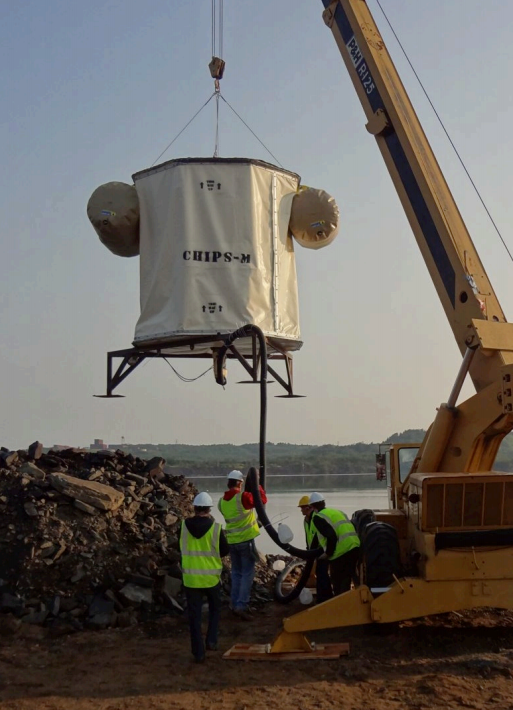
\includegraphics[width=0.6\textwidth]{diagrams/4-chips/chips_m.png}
    \caption[Picture of the \chipsm detector.]
    {Picture of the \unit{3.3}{\mathrm{m}} high \chipsm detector just before deployment. The
        temporary floatation bags are visibly attached to the top rim of the detector.
        Additionally, the umbilical cord carrying data, power, and filtered water is attached to
        the bottom of the detector.}
    \label{fig:chips_m}
\end{figure}

\subsection{The neutrino beam and off-axis alignment} %%%%%%%%%%%%%%%%%%%%%%%%%%%%%%%%%%%%%%%%%%%%
\label{sec:chips_concept_beam} %%%%%%%%%%%%%%%%%%%%%%%%%%%%%%%%%%%%%%%%%%%%%%%%%%%%%%%%%%%%%%%%%%%

\chips detectors will primarily study the appearance of $\nu_{e}$ oscillating from $\nu_{\mu}$
over a long-baseline. To generate a sufficient number of GeV scale $\nu_{\mu}$, a high-intensity
accelerator beam is required. Currently, only two such beams exist, the J-PARC based beam in Japan
used by the T2K experiment and the \numi beam in the USA used by \nova. Here we describe the
\numi~\cite{adamson2016} (Neutrinos at the Main Injection) beam as it is directly relevant to
current \chips efforts. However, it is essential to note that \chips detectors are designed to be
used in any neutrino beam, including the future \numi replacement, LBNF.

The \numi beam is an accelerator muon neutrino beam produced at Fermilab near Chicago in the USA.
Beginning operation in 2005 for the MINOS experiment, \numi was upgraded in 2013 to provide a
higher intensity and energy, principally to achieve a peak in neutrino energy near the
$\sim$\unit{1.5}{\GeV} $\nu_{\mu}\rightarrow\nu_{e}$ oscillation maximum for \nova. Currently the
\numi beam achieves an intensity above \unit{700}{\mathrm{kW}} (\unit{740}{\mathrm{kW}} peak)
making it the most powerful such beam in the world. A schematic of the \numi beamline
configuration is shown in Fig.~\ref{fig:numi_beam}.

\begin{figure} % NUMI BEAM DIAGRAM %
    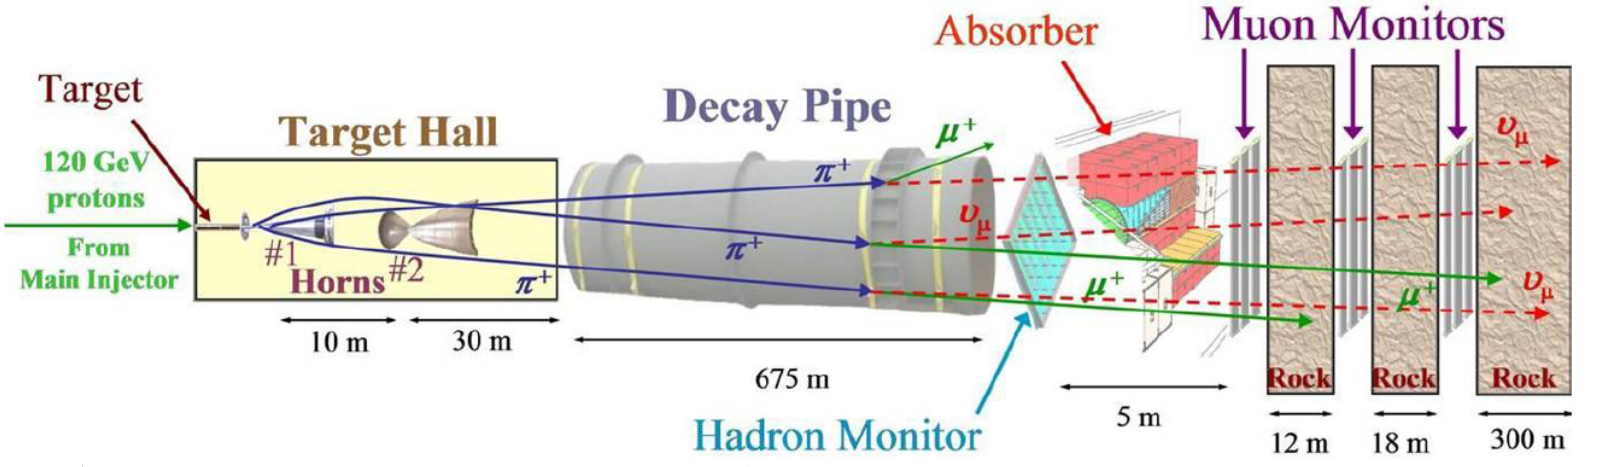
\includegraphics[width=\textwidth]{diagrams/4-chips/numi_beam.png}
    \caption[Schematic of the main components of the \numi beam.]
    {Schematic of the main components of the \numi beam (not to scale) shown with dimensions. The
        MINOS and \nova near detectors and the MINERvA experiment are located just to the right
        of what is shown. Figure taken from Ref.~\cite{adamson2016}.}
    \label{fig:numi_beam}
\end{figure}

Every \unit{1.33}{\mathrm{seconds}} a \unit{10}{\mu\mathrm{s}} long spill of protons accelerated
to \unit{120}{\GeV} by the Main Injector ring are directed towards a stationary graphite target.
The resulting interactions within the target create a shower of secondary hadrons containing
predominantly pions and kaons. The hadrons are passed through a focusing system of two magnetic
horns tuned principally to focus charged pions along the beamline while rejecting other particles.
After focusing, the surviving hadrons are allowed to decay in flight to a beam of muon neutrinos
in a \unit{675}{\mathrm{m}} long decay pipe via the processes,
\begin{align} % NUMI DECAY EQUATIONS %
    \pi^{+} & \rightarrow\mu^{+}+\nu_{\mu}, \label{eq:pi_decays}   \\
    K^{+}   & \rightarrow\mu^{+}+\nu_{\mu}. \label{eq:kaon_decays}
\end{align}
The resulting muons also decay such that $\mu^{+}\rightarrow e^{+}+\nu_{e}+\bar{\nu}_{\mu}$
producing an intrinsic $\nu_{e}$ background as well as wrong sign $\nu_{\mu}$ contamination.

Alternatively, the polarity of the horns can be used to switch the dominant sign of the hadrons
focused, allowing \numi to operate as either a neutrino or antineutrino beam. These two modes of
operation are called \emph{forward horn current} and \emph{reverse horn current} for primarily a
neutrino or antineutrino beam composition respectively. Any remaining hadrons, alongside
electrons, muons and surviving primary protons are absorbed by rock downstream of the decay pipe,
leaving just the neutrino components of the beam.

Long-baseline neutrino experiments typically consist of a \emph{near detector} to measure the beam
neutrino composition at source and a much larger \emph{far detector} to measure the oscillated
composition at many hundreds of kilometres. The \numi beamline contains three detectors just
downstream of \unit{300}{\mathrm{m}} of rock: The MINERvA spectrometer~\cite{mcfarland2006}, the
near detector for MINOS (now used by MINERvA), and the near detector for \nova. \chips prototypes
within the \numi beam will not have a dedicated near detector; therefore, data from the above
detectors will be crucial for physics analysis in order to constrain the beam composition and
flux.

The \numi neutrino beam passes through the Earth's crust until it finally emerges in northern
Minnesota. This is where the MINOS, \nova, and prototype \chips far detectors are located (used to
be located in the MINOS case), as shown in Fig.~\ref{fig:numi_map}. The Minnesota state nickname
`land of 10,000 lakes' is not an overstatement, with a vast number of potential lakes for \chips
detector deployment. Additionally, intense iron ore mining on the `Iron Range' provides many
suitable disused (and now flooded) mine pits. The exact \chipsfive prototype detector location is
discussed in greater detail in Section.~\ref{sec:chips_detector}.

\begin{figure} % CHIPS LOCATION IN NUMI DIAGRAM %
    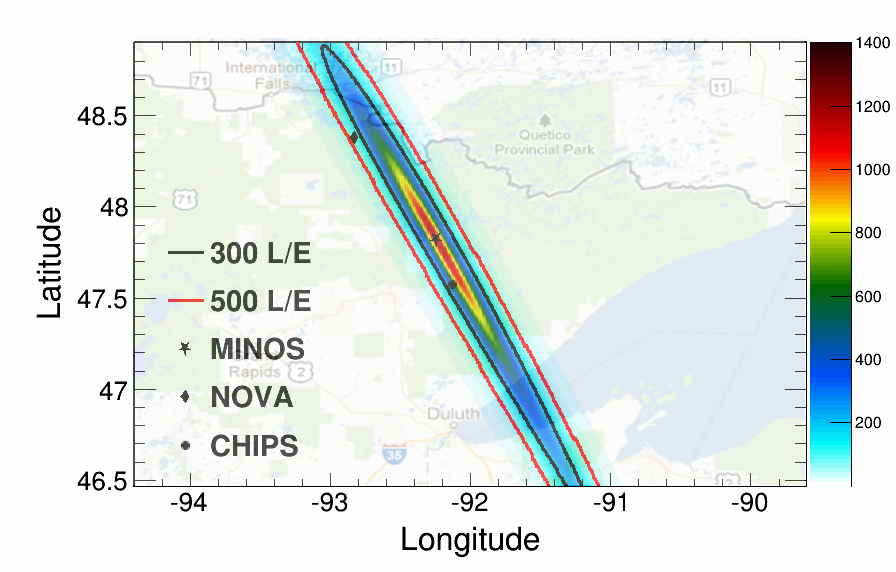
\includegraphics[width=0.7\textwidth]{diagrams/4-chips/numi_map.png}
    \caption[Map of detector locations in the \numi beam.]
    {Map of the MINOS, \nova and \chips locations in the \numi beam as it surfaces in northern
        Minnesota. Shown is the expected neutrino event rate assuming no oscillations, with lines
        of constant L/E indicated by contours. The western extent of Lake Superior can be seen in
        the lower right of the map. Image taken from Ref.\cite{adamson2013}.}
    \label{fig:numi_map}
\end{figure}

Due to the kinematics of pion decay, whether the far detector is placed directly on the beam axis
or not can have a significant impact on the observed energy spectrum of beam neutrinos as shown in
Fig.~\ref{fig:numi_axis}. For neutrinos directly on the beam axis, there is a strong energy
dependence on the parent pion energy from Eq.~\ref{eq:pi_decays}. However, as the off-axis angle
increases, the neutrino energy becomes less dependent on the parent pion energy and is restricted
to a narrowing range of decreasing energies. This effect known as the \emph{off-axis effect} is
used by both \nova and T2K to create a narrower energy spectrum focused on the
$\nu_{\mu}\rightarrow\nu_{e}$ oscillation maximum. Additionally, by reducing the tail of
higher-energy neutrinos, the number of background NC events can be greatly reduced, as is the case
for the \unit{7}{\mathrm{mrad}} off-axis \chipsfive prototype detector.

\begin{figure} % OFF-AXIS FLUX DIAGRAM %
    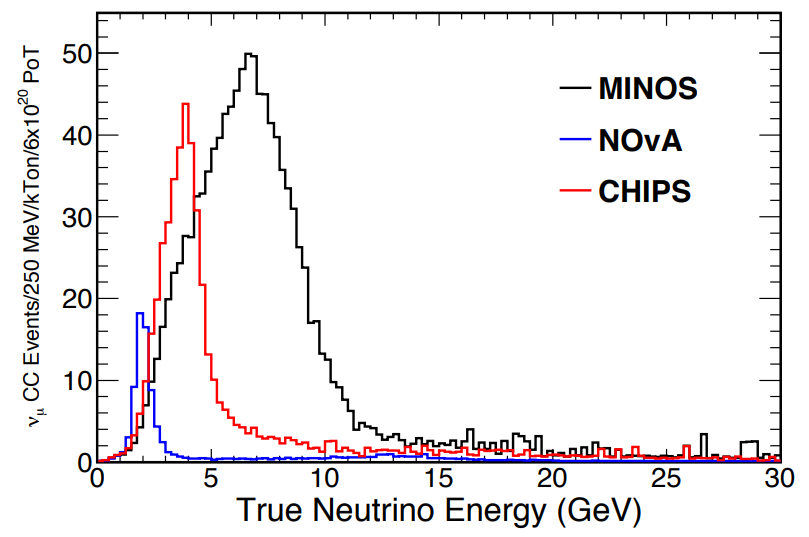
\includegraphics[width=0.6\textwidth]{diagrams/4-chips/numi_axis.png}
    \caption[Muon neutrino flux for different \numi detectors at different off-axis angles.]
    {Muon neutrino flux for different \numi detectors at different off-axis angles. Shown are the
        neutrino energy spectrum for MINOS (on-axis), \nova (\unit{14}{\mathrm{mrad}} off-axis),
        and \chipsfive (\unit{7}{\mathrm{mrad}} off-axis). Figure taken from
        Ref.~\cite{adamson2013}.}
    \label{fig:numi_axis}
\end{figure}

\subsection{Water Cherenkov detectors} %%%%%%%%%%%%%%%%%%%%%%%%%%%%%%%%%%%%%%%%%%%%%%%%%%%%%%%%%%%
\label{sec:chips_concept_cherenkov} %%%%%%%%%%%%%%%%%%%%%%%%%%%%%%%%%%%%%%%%%%%%%%%%%%%%%%%%%%%%%%

The \chips detector concept is based upon the water Cherenkov technique for neutrino detection. A
large body of target water is instrumented with photomultiplier tubes (PMTs) to record the
Cherenkov radiation produced by sufficiently relativistic charged particles resulting from
neutrino interactions. By using readily available water as the target material and only
instrumenting the volume surface, water Cherenkov detectors provide the best detection methodology
for maximising volume and reducing cost.

Cherenkov radiation is emitted by all electrically charged particles travelling faster than the
local phase velocity of light in a dielectric medium. Similar to the sonic boom created by a
supersonic aircraft, Cherenkov radiation forms a shock wave of coherent light, as shown in
Fig.~\ref{fig:cherenkov}. Typically the emitted light has wavelengths in the optical to
ultraviolet range. When projected onto the detector wall, the resulting cone of radiation
generates a distinctive ring shape. The cone opening angle (the angle at which light is emitted)
$\theta_{c}$ is given by:
\begin{equation}
    \cos\theta_{c} = \frac{1}{\beta n(\lambda)},
    \label{eq:cherenkov_angle}
\end{equation}
where $\beta=v/c$ and $n$ is the refractive index of the medium~\cite{particle2020}. Note that $n$
is a function of the wavelength of emission $\lambda$, and so is the opening angle. As the
refractive index of water is $\sim 1.33$ for typical wavelengths of emission, and using the
ultrarelativistic limit $\beta\sim 1$ the opening angle is found to be $\sim41^{\circ}$.

\begin{figure} % CHERENKOV EFFECT DIAGRAM DIAGRAM %
    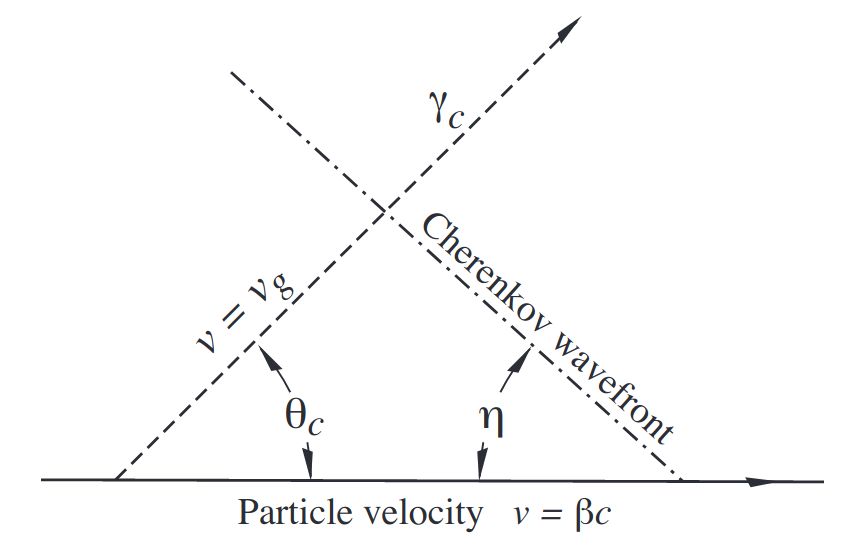
\includegraphics[width=0.6\textwidth]{diagrams/4-chips/cherenkov.png}
    \caption[Diagram of Cherenkov radiation emission.]
    {Diagram of Cherenkov radiation emission and wavefront angles. The angles $\theta_{c}$ and
        $\eta$ are not equal in a dispersive medium. Figure taken from Ref.~\cite{particle2020}}
    \label{fig:cherenkov}
\end{figure}

In Eq.~\ref{eq:cherenkov_angle} there is no Cherenkov emission when $\cos\theta_{c} > 1$, which is
the case when $\beta n(\lambda)<1$. Therefore, a Cherenkov energy threshold $E_{t}$ exists for
charged particle, which when expressed in terms of the particle mass $m$ is given by:
\begin{equation}
    E_{t} = \gamma m = \frac{m}{\sqrt{1-(1/n)^{2}}}.
    \label{eq:cherenkov_threshold}
\end{equation}
Again using $n\sim 1.33$, a threshold energy of $\sim1.5m$ is typical.

The number of Cherenkov photons emitted by a particle of charge $ze$ per unit wavelength per unit
path length is given by:
\begin{equation}
    \frac{d^{2}N}{d\lambda dx}=\frac{2\pi\alpha z^{2}}{\lambda^{2}}
    \left(1-\frac{1}{1-\beta^{2}n^{2}(\lambda)}\right),
    \label{eq:cherenkov_emission}
\end{equation}
where $\alpha$ is the fine structure constant~\cite{particle2020}. Integrating over the range of
wavelengths for which PMTs are typically sensitive, \unit{350}{\mathrm{nm}} to
\unit{650}{\mathrm{nm}}, and using $\beta\sim 1$ and $n\sim 1.33$ gives $\sim240$ photons emitted
per cm travelled by the charged particle~\cite{perch2017}.

By analysing the Cherenkov ring (or rings) of light recorded by the PMTs on the walls of the
detector, information about the charged particle (particles) within an event can be determined.
The underlying neutrino interaction can then be understood indirectly. Primarily the challenge for
accelerator beam water Cherenkov detectors is the identification and reconstruction of an electron
or muon ring likely to have been produced from a beam neutrino and not a cosmic ray. This event
topology indicates a beam CC $\nu_{e}$ or CC $\nu_{\mu}$ event respectively, rejecting NC and
cosmic events.

The basic shape of a Cherenkov ring can be used to tell which charged particle created it. Muons
are long-lived and typically travel many metres within the detector, producing a clean ring with
sharp edges. Conversely, electrons almost immediately initiate an electromagnetic shower;
therefore, the observed ring is the sum of all the rings produced from the individual electrons
and positrons within the shower. As a consequence, when compared to a muon ring, electron rings
are characteristically fuzzy. A factor of this difference can be seen in Fig.~\ref{fig:emission
    distance}, which shows how the total amount of Cherenkov radiation is emitted for both electrons
and muons as a function of distance from the interaction vertex.

\begin{figure} % EMISSION DISTANCE DIAGRAM %
    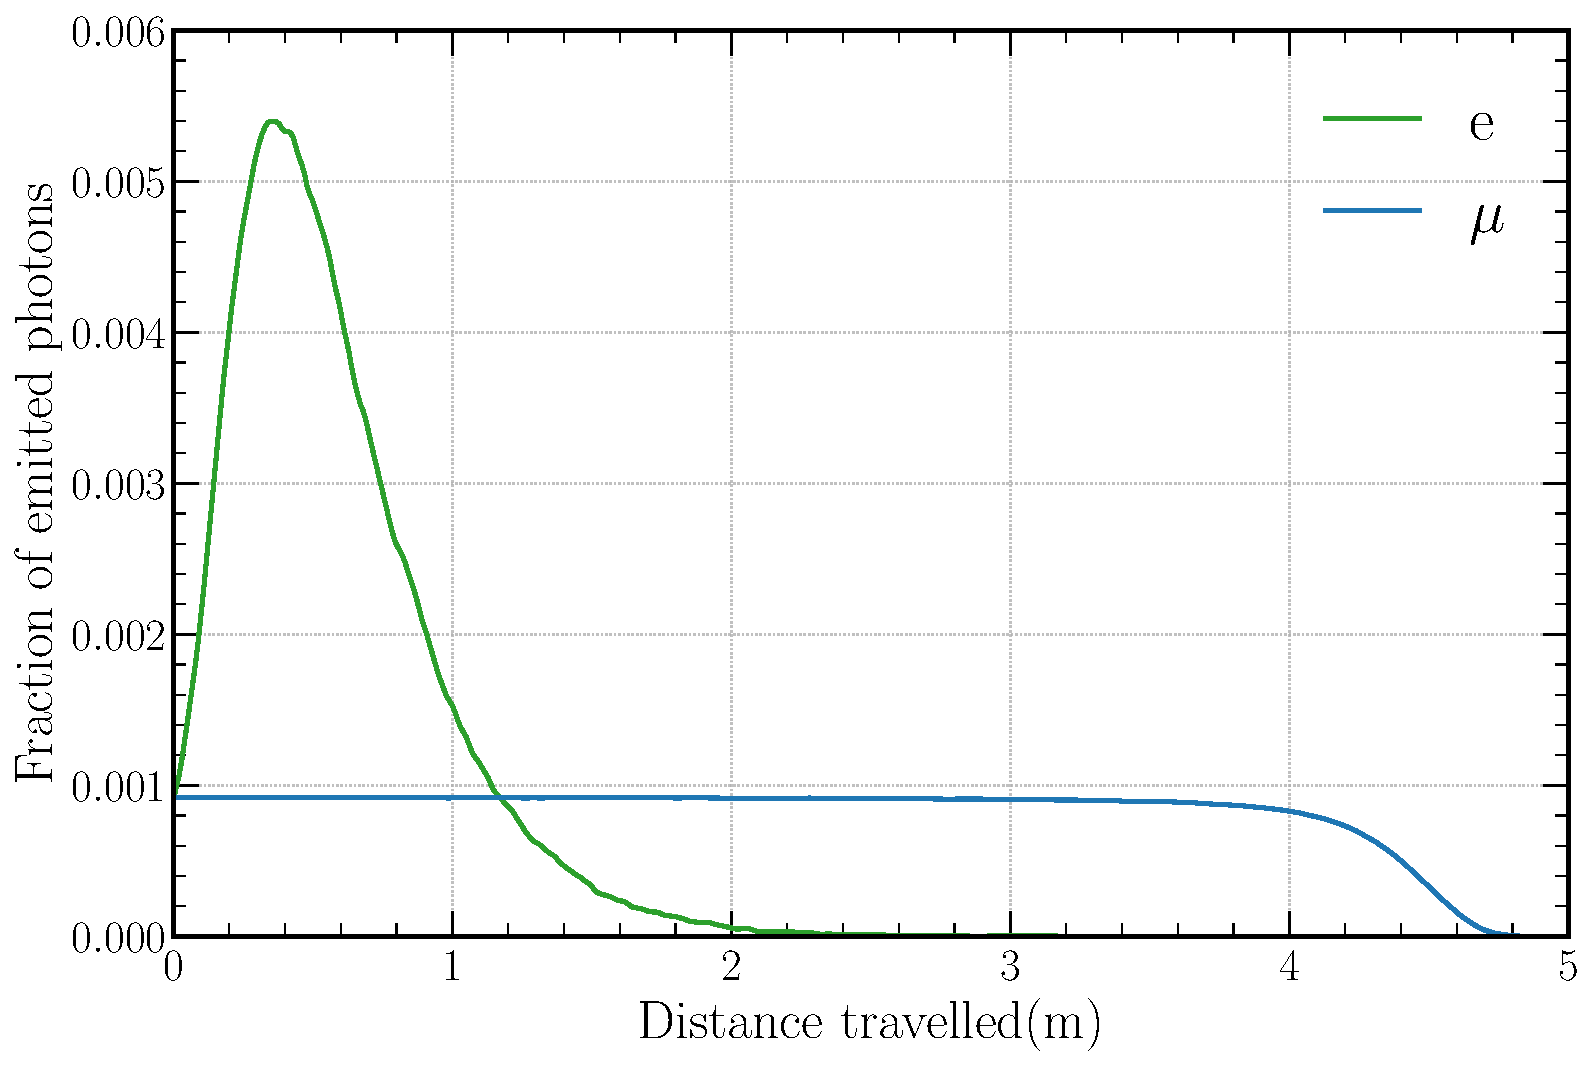
\includegraphics[width=0.6\textwidth]{diagrams/4-chips/emission_distance.pdf}
    \caption[Fraction of Cherenkov photons emitted as a function of distance.]
    {The fraction of the total number of photons emitted as a function of the distance from the
        interaction vertex for both electrons and muons with energy of \unit{2.5}{\GeV}. Multiple
        particles within the electron induced electromagnetic shower emit their Cherenkov
        radiation over a short distance and in slightly different directions. Conversely, a muon
        travels relatively much further emitting an approximately constant level of Cherenkov
        radiation as it does so, leading to a clean, sharp-edged ring.}
    \label{fig:emission distance}
\end{figure}

The situation becomes complicated when multiple charged particles above the Cherenkov threshold
are involved, common at multi-$\GeV$ energies. In this case, multiple overlapping rings are
observed, making reconstruction difficult. The worst-case scenario, however, is when two rings
entirely overlap, removing any ability to tell them apart. This topology is commonly the case for
NC interactions producing a $\pi^{0}$ in the final state, forming the primary background for CC
$\nu_{e}$ appearance.

$\pi^{0}$ particles decay to a pair of photons with a 98.82\% branching ratio, both which almost
immediately initiate an electromagnetic shower, just like an electron~\cite{particle2020}. This
process leads to two, electron like rings to be observed with a separation angle given by:
\begin{equation}
    (1-\cos\theta_{ij})=\frac{m_{\pi}^2}{2E_{i}E_{k}},
\end{equation}
where $m_{\pi}$ is the invariant mass of the $\pi^{0}$ and $E_{i}$ and $E_{j}$ are the energies of
the two photons respectively. Therefore, for a $\pi^{0}$ decaying to two \unit{1}{\GeV} photons,
there is just $\sim 8^{\circ}$ of separation between the rings, making them difficult to tell
apart. This distinction is especially hard when electron like rings are also fuzzy. Alternatively,
if the two photons have an unequal energy distribution, such that one is much more energetic than
the other, the higher energy photon ring can dominate, and the other can not be identified,
leading to what looks like a single electron ring, again a misidentification.

\section{The \chipsfive detector} %%%%%%%%%%%%%%%%%%%%%%%%%%%%%%%%%%%%%%%%%%%%%%%%%%%%%%%%%%%%%%%%
\label{sec:chips_detector} %%%%%%%%%%%%%%%%%%%%%%%%%%%%%%%%%%%%%%%%%%%%%%%%%%%%%%%%%%%%%%%%%%%%%%%

\chipsfive is the first large scale prototype detector module for the \chips project. A
\unit{25}{\mathrm{m}} wide and \unit{12}{\mathrm{m}} high cylinder once fully deployed, \chipsfive
has an inner surface area of \unit{1924}{\mathrm{m}^2} and a total target mass
\unit{5.9}{\mathrm{kton}}. Via the process of design, construction, deployment, and data taking,
\chipsfive primarily aims to refine the \chips concept for future full-scale
($\sim$\unit{15}{\mathrm{kton}}) modules. Consequently, \chipsfive is designed such that the
details outlined in this section are fully characteristic of what a full-sized \chips module is
envisioned to be. Here, the location, structure, instrumentation, water filtration, deployment,
and current status are presented. The full electronics and DAQ details are outlined in
Chapter.~\ref{chap:daq}.

\subsection{Location} %%%%%%%%%%%%%%%%%%%%%%%%%%%%%%%%%%%%%%%%%%%%%%%%%%%%%%%%%%%%%%%%%%%%%%%%%%%
\label{sec:chips_detector_location} %%%%%%%%%%%%%%%%%%%%%%%%%%%%%%%%%%%%%%%%%%%%%%%%%%%%%%%%%%%%%

\chipsfive is located at the Wentworth 2W pit in northern Minnesota, USA, near the small town of
Hoyt Lakes. A disused and flooded surface Taconite ore (a type of iron ore) mine pit, Wentworth 2W
is located \unit{7}{\mathrm{mrad}} off the \numi axis at a distance of \unit{712}{\mathrm{km}}
from the beam target. Roughly \unit{0.8}{\mathrm{km}}$\times$\unit{1.2}{\mathrm{km}} in size with
a maximum depth of \unit{60}{\mathrm{m}} ($\pm3\mathrm{m}$ throughout the year), the pit allows
for an overburden of approximately \unit{50}{\mathrm{m}} with \chipsfive resting at the bottom.
With an average daily low temperate of $-24^{\circ}\mathrm{C}$ in January, the pit freezes over
during the winter months, therefore, work is only possible during the summer months of May to
October.

A sizeable earthen ramp on the south side of the Wentworth 2W pit is used for construction on
land. The construction site is easily accessible by road and well connected to power, due to the
heavy infrastructure in place for mining. Additionally, the nearby PolyMet mining administration
building is used as a laboratory environment for construction and testing of individual components
before installation within the detector. A labelled satellite view of Wentworth 2W is given in
Fig.~\ref{fig:pit} for context, with a picture of the construction site shown in
Fig.~\ref{fig:from_the_sky}.

\begin{figure} % PIT DIAGRAM %
    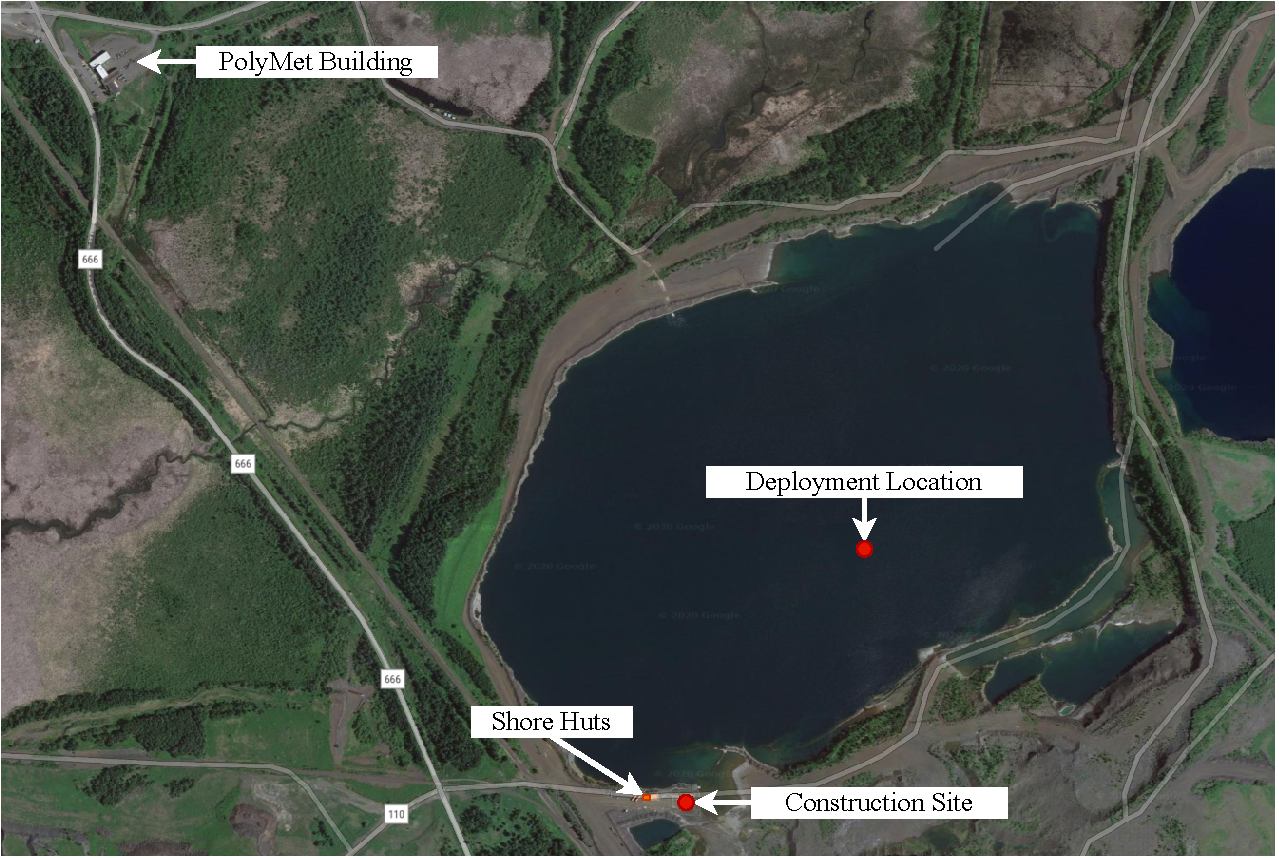
\includegraphics[width=\textwidth]{diagrams/4-chips/pit.pdf}
    \caption[Satellite view of the Wentworth 2W mine pit, with key locations.]
    {Satellite view of the Wentworth 2W flooded mine pit in northern Minnesota, showing key
        \chipsfive locations. The PolyMet building, shore huts, construction site and deployment
        location are shown. For both the construction site and deployment location the red circle
        shows the \chipsfive detector size to scale.}
    \label{fig:pit}
\end{figure}

\begin{figure} % CHIPS FROM THE SKY DIAGRAM %
    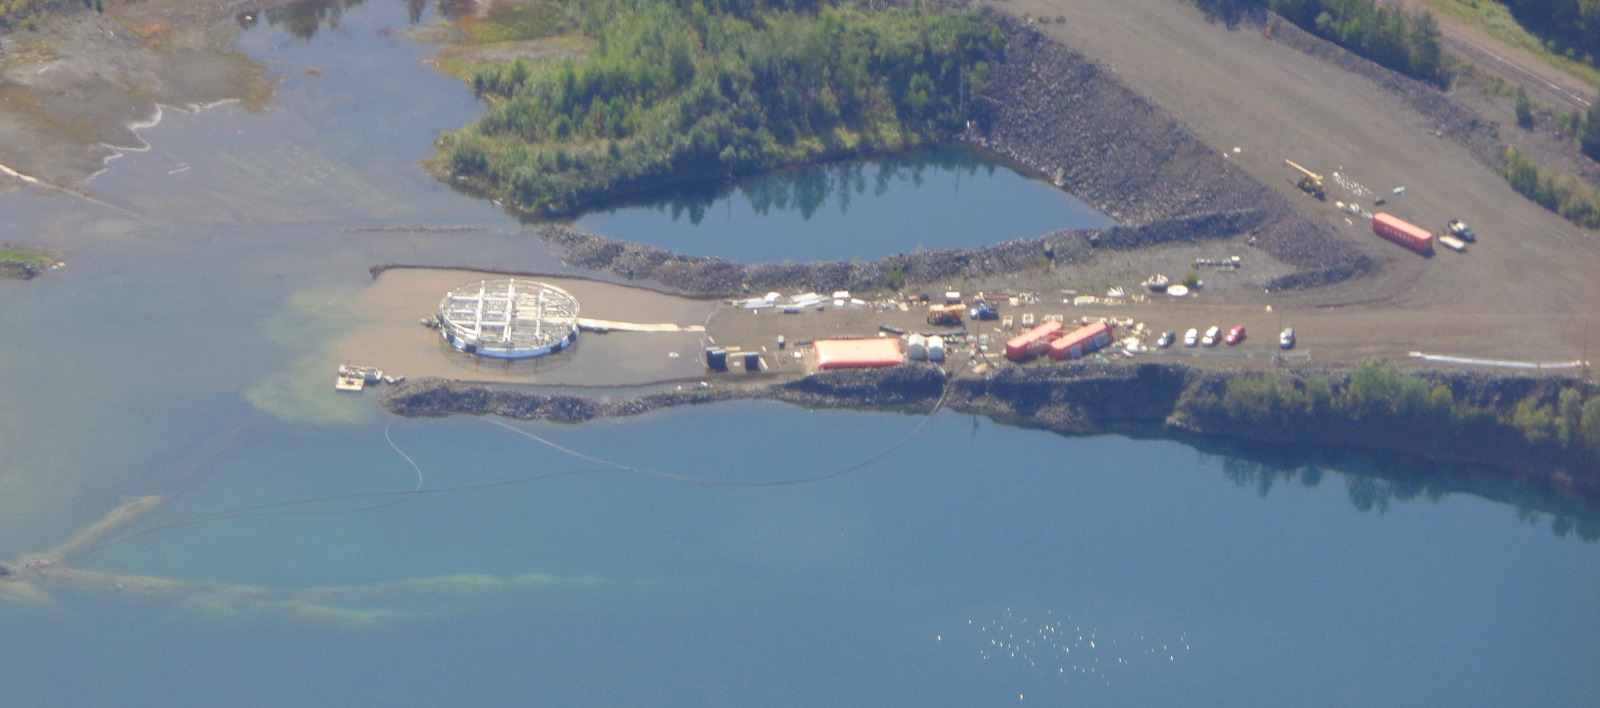
\includegraphics[width=\textwidth]{diagrams/4-chips/from_the_sky.jpg}
    \caption[Picture of the \chipsfive construction site from the air.]
    {Picture of the \chipsfive construction site from the air facing south. The Wentworth 2W pit
        is in the lower half of the image, with the part built \chipsfive detector visible at the
        bottom of the earthen construction ramp. The two white shore huts can just be seen halfway
        up the ramp.}
    \label{fig:from_the_sky}
\end{figure}

\subsection{Structure} %%%%%%%%%%%%%%%%%%%%%%%%%%%%%%%%%%%%%%%%%%%%%%%%%%%%%%%%%%%%%%%%%%%%%%%%%%%
\label{sec:chips_detector_structure} %%%%%%%%%%%%%%%%%%%%%%%%%%%%%%%%%%%%%%%%%%%%%%%%%%%%%%%%%%%%%

The structure of the \chipsfive detector module consists primarily of two \unit{26}{\mathrm{m}}
diameter and \unit{1.3}{\mathrm{m}} high lightweight stainless steel circular \emph{endcaps} that
form the top and bottom of the cylinder. During construction on land the conveniently named
\emph{top-cap} is held above the \emph{bottom-cap} by \unit{1.5}{\mathrm{m}} long steel struts as
shown in Fig.~\ref{fig:frame}. This configuration allows for the endcap instrumentation, detailed
in Section.~\ref{sec:chips_detector_instrumentation}, to be easily installed.

\begin{figure} % CHIPS FRAME DIAGRAM %
    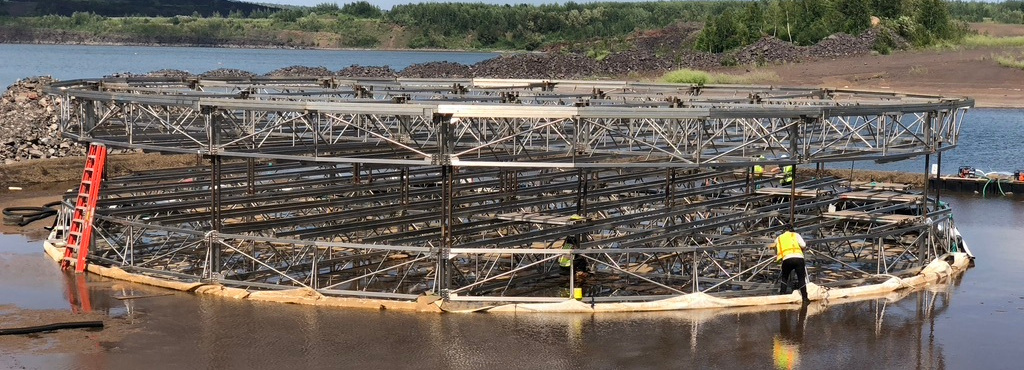
\includegraphics[width=\textwidth]{diagrams/4-chips/frame.jpeg}
    \caption[Picture of the \chipsfive structural frame.]
    {Picture of the \chipsfive structural frame, with humans for scale. The top and bottom endcaps
        can be seen separated by steel struts. Rows of stainless steel \emph{stringers}
        are attached to the inside of each endcap to mount the instrumentation.}
    \label{fig:frame}
\end{figure}

The two endcaps are connected by 28 \unit{12}{\mathrm{m}} long Dyneema cables around their
perimeter. Additionally, 48 \unit{16}{\mathrm{inch}} diameter air-filled PVC pipes are attached to
the frame of the top-cap, making it buoyant. Therefore, once deployed into the pit, the bottom-cap
sinks while the top-cap floats, this pulls the Dyneema cable until taut, forming the final
expanded detector shape, as shown in Fig.~\ref{fig:chips_render}.

\begin{figure} % CHIPS RENDER DIAGRAM %
    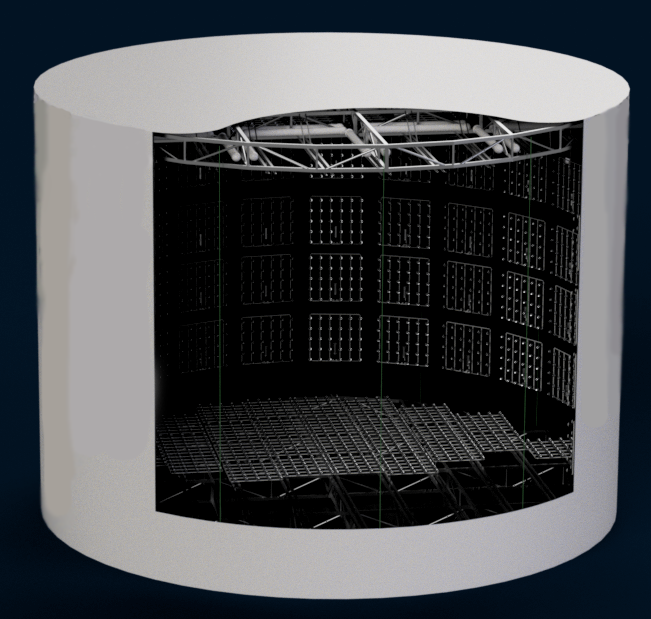
\includegraphics[width=0.6\textwidth]{diagrams/4-chips/chips_render_1.png}
    \caption[Graphical rendering of the \chipsfive detector.]
    {Graphical rendering of the fully deployed and expanded \chipsfive detector module with a
        section of the liner cutaway. The bottom endcap and wall planes are visible, as well as
        the top endcap structure and floatation. The green lines indicate the Dyneema cables
        holding the top-cap and bottom-cap together.}
    \label{fig:chips_render}
\end{figure}

A lightproof and watertight liner is also installed to surround the fully expanded structure.
Designed to isolate the clean internal water from the external pit water and to prevent
non-Cherenkov light from reaching the PMTs, the liner is made from geomembrane, a flexible
reinforced polymer membrane. Commercially available in large rolls the liner is welded together
during construction to form the top, bottom, and sides. Note that when fully deployed, the liner
does not take any of the structural strain.

\subsection{Instrumentation} %%%%%%%%%%%%%%%%%%%%%%%%%%%%%%%%%%%%%%%%%%%%%%%%%%%%%%%%%%%%%%%%%%%%%
\label{sec:chips_detector_instrumentation} %%%%%%%%%%%%%%%%%%%%%%%%%%%%%%%%%%%%%%%%%%%%%%%%%%%%%%%

The \chipsfive detector is instrumented with PMTs arranged within distinct plane like structures
called Planar Optical Modules (POMs), which take inspiration from the Digital Optical Modules
(DOMs) used by IceCube and KM3NeT~\cite{hanson2006, eijk2015}. Each POM is a roughly
\unit{2}{\mathrm{m}}$\times$\unit{3}{\mathrm{m}} array of watertight PVC tubing equipped with
anywhere between $15$ to $30$ PMTs, in addition to the lowest level of DAQ electronics and power
distribution. Standard commercially available schedule $40$ PVC piping and connectors are used to
form the structure of each plane, bound together with PVC primer and cement.

There are two types of POM used within \chipsfive, differentiated by the PMTs and the data
acquisition electronics they use and named after the institution at which they were developed.
Firstly, \emph{Nikhef} POMs use \unit{88}{\mathrm{mm}} HZC PMTs with electronics developed by the
KM3NeT experiment~\cite{katz2009, adrian2016}. Secondly, \emph{Madison} POMs use
\unit{3}{\mathrm{inch}} Hamamatsu R6091 PMTs donated from the NEMO3 experiment~\cite{arnold2005}
with novel electronics developed by \chips in collaboration with the Wisconsin IceCube Particle
Astrophysics Centre (WIPAC) in Madison, Wisconsin. The \unit{88}{\mathrm{mm}} HZC PMTs have a high
ratio of output electrons to incident photons (quantum efficiency) of 24.4\% at a wavelength of
\unit{400}{\mathrm{nm}}, compared to the low 12.0\% ratio achieved by the R6091 PMTs. Furthermore,
the first photon time resolution is $\sim2\mathrm{ns}$ and $\sim5\mathrm{ns}$ for
\unit{88}{\mathrm{mm}} HZC and R6091 PMTs respectively.

In total $6114$ \unit{88}{\mathrm{mm}} HZC and $450$ Hamamatsu R6091 PMTs are arranged into $226$
Nikhef and $30$ Madison POMs. Every PMT is housed in an assembly as shown in
Fig.~\ref{fig:nikhef_pmt_assembly} for the Nikhef case and Fig.~\ref{fig:madison_pmt_assembly} for
the Madison case. Importantly, to increase the level of light collection, each Nikhef PMT is
equipped with a \emph{light-cone} consisting of a circular reflective surface at \unit{45}{^\circ}
to the PMT normal. The Madison PMT assembly is similar but has no cover or light cone. For POMs
attached to either endcap, their PMTs are angled at \unit{45}{^\circ} facing the direction of the
beam to increase light collection furthermore.

All PMTs within a POM are connected to the lowest level of DAQ electronics contained within a
dedicated electronics box. Either an aluminium or PVC cylinder in the Nikhef or Madison case
respectively. A flexible PVC \emph{pigtail} is attached to each POM electronics box containing
connections to the higher level DAQ and power supply. A \emph{water-block} within each pigtail
ensures that even if the outside connection is flooded, every POM is capable of withstanding the
\unit{6}{\mathrm{atm}} of water pressure at the bottom of the pit. A fully assembled and installed
Nikhef POM is shown in Fig.~\ref{fig:single_plane} for reference.

\begin{figure} % NIKHEF PMT ASSEMBLY DIAGRAM %
    \centering
    \subcaptionbox{Disassembled}{%
        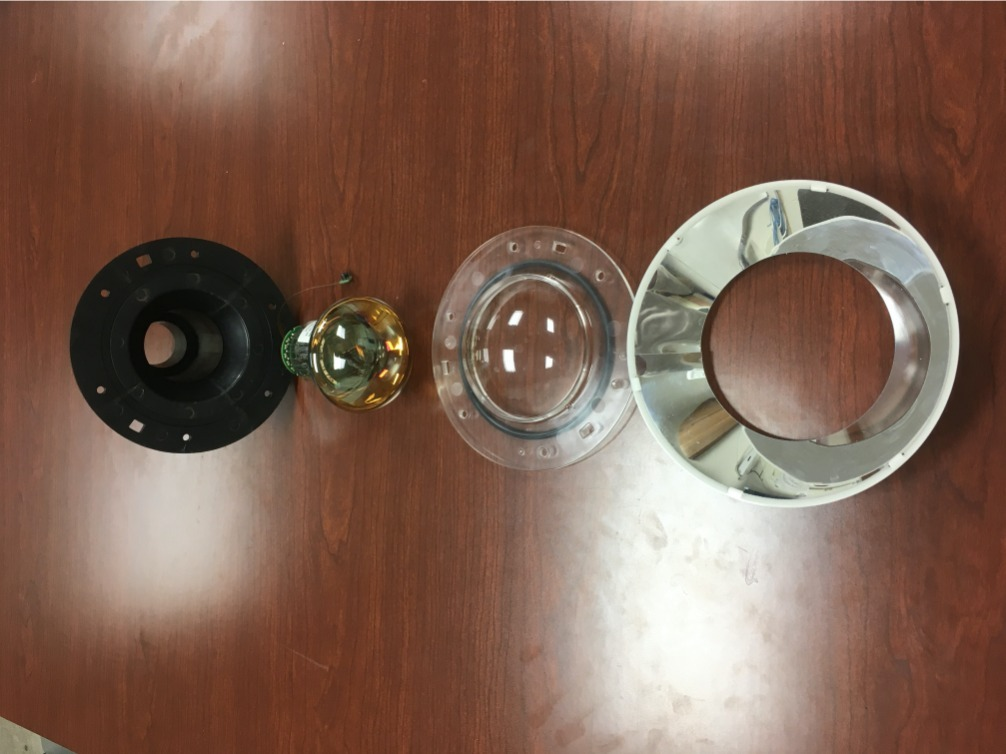
\includegraphics[height=5.5cm]{diagrams/4-chips/pmt_disassembled.jpg}%
    }
    \quad
    \subcaptionbox{Assembled}{%
        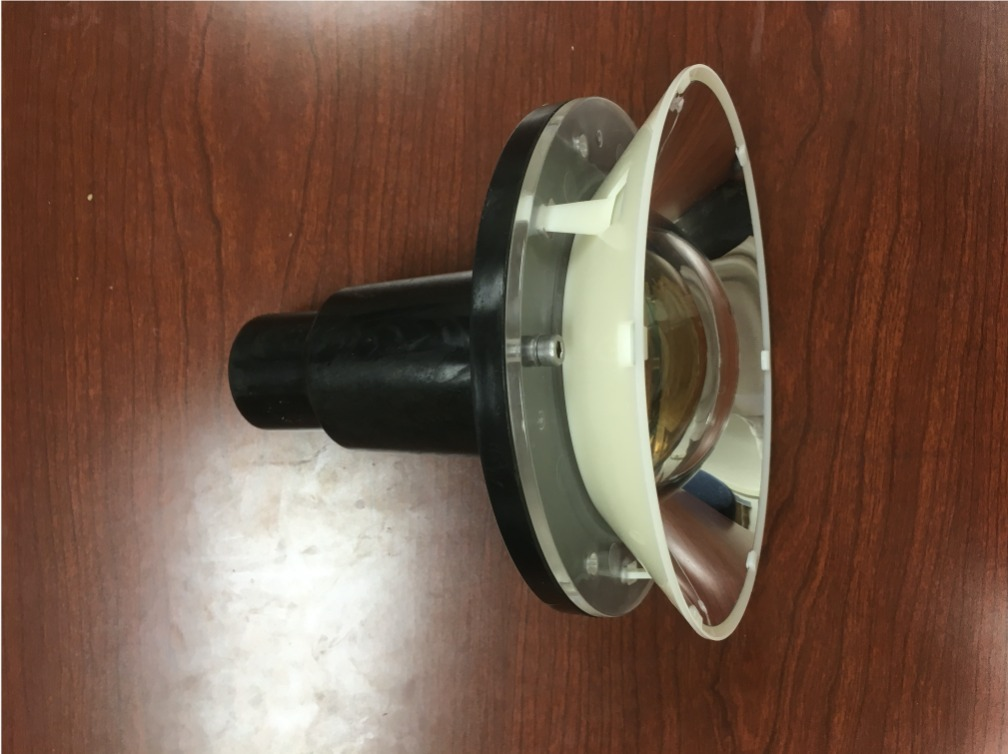
\includegraphics[height=5.5cm]{diagrams/4-chips/pmt_assembled.jpg}%
    }
    \caption[Disassembled and assembled Nikhef PMT housing components.]
    {Disassembled (a) and assembled (b) Nikhef PMT assembly components. The assembly comprises of
        a black PVC insert, a \unit{88}{\mathrm{mm}} HZC PMT, a transparent acrylic cover, and a
        reflective light cone. The PMT is glued to the inside surface of the cover using a
        silicone-based optical gel and a watertight seal is made between the insert and cover
        using an O-ring. The reflective light cone is clipped to the front of the cover and the
        whole assembly is glued into the POM PVC structure.}
    \label{fig:nikhef_pmt_assembly}
\end{figure}

\begin{figure} % MADISON PMT ASSEMBLY DIAGRAM %
    \centering
    \subcaptionbox{Outside}{%
        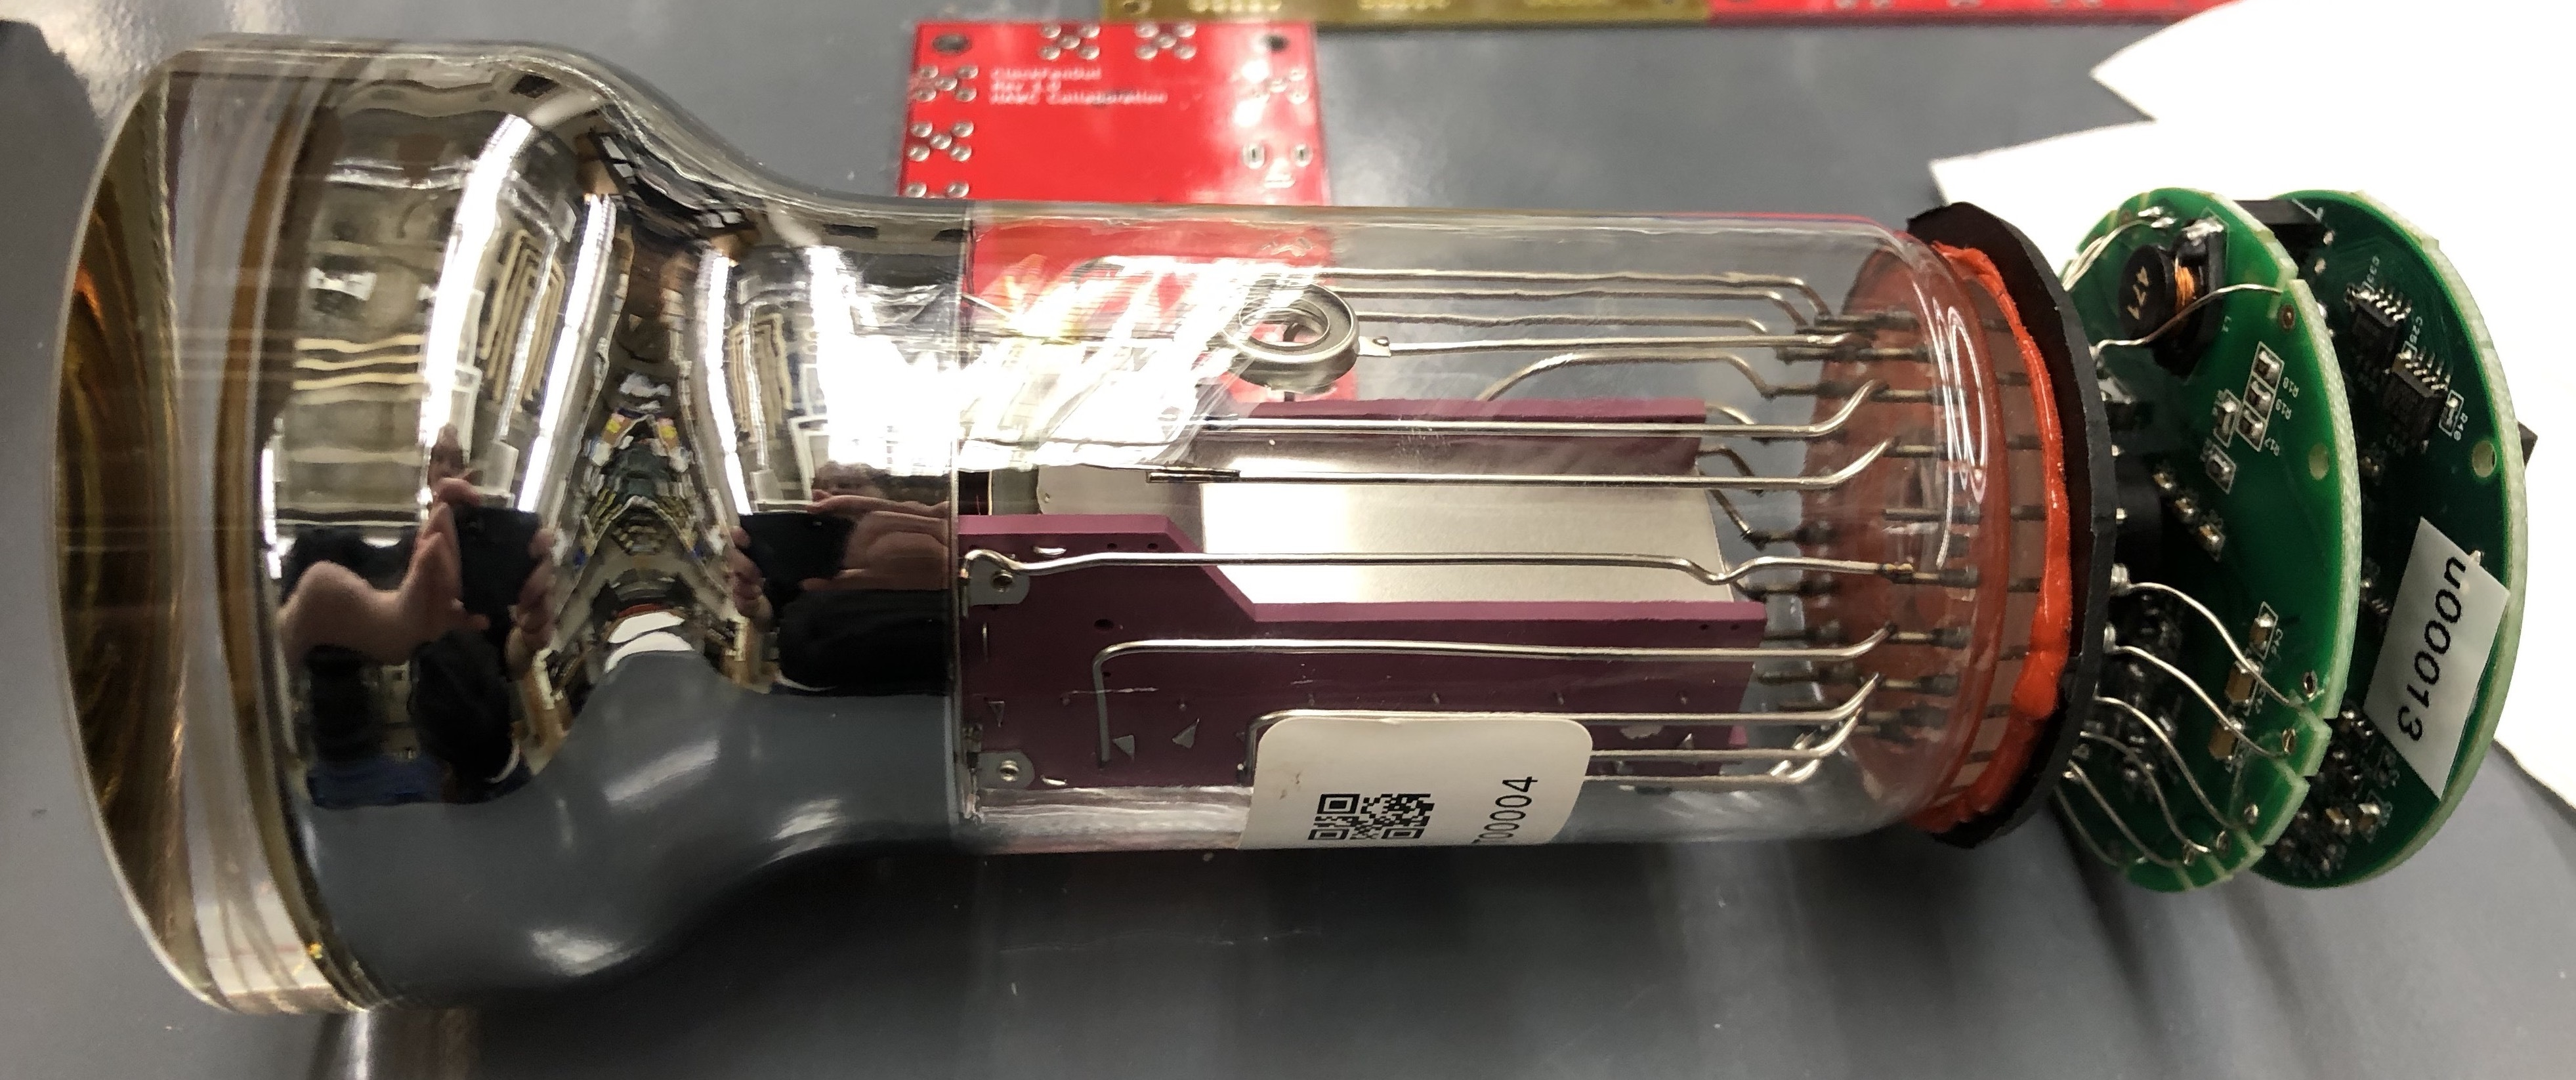
\includegraphics[angle=270,origin=c,height=4.3cm]{diagrams/4-chips/madison_pmt.jpeg}%
    }
    \quad
    \subcaptionbox{Inside}{%
        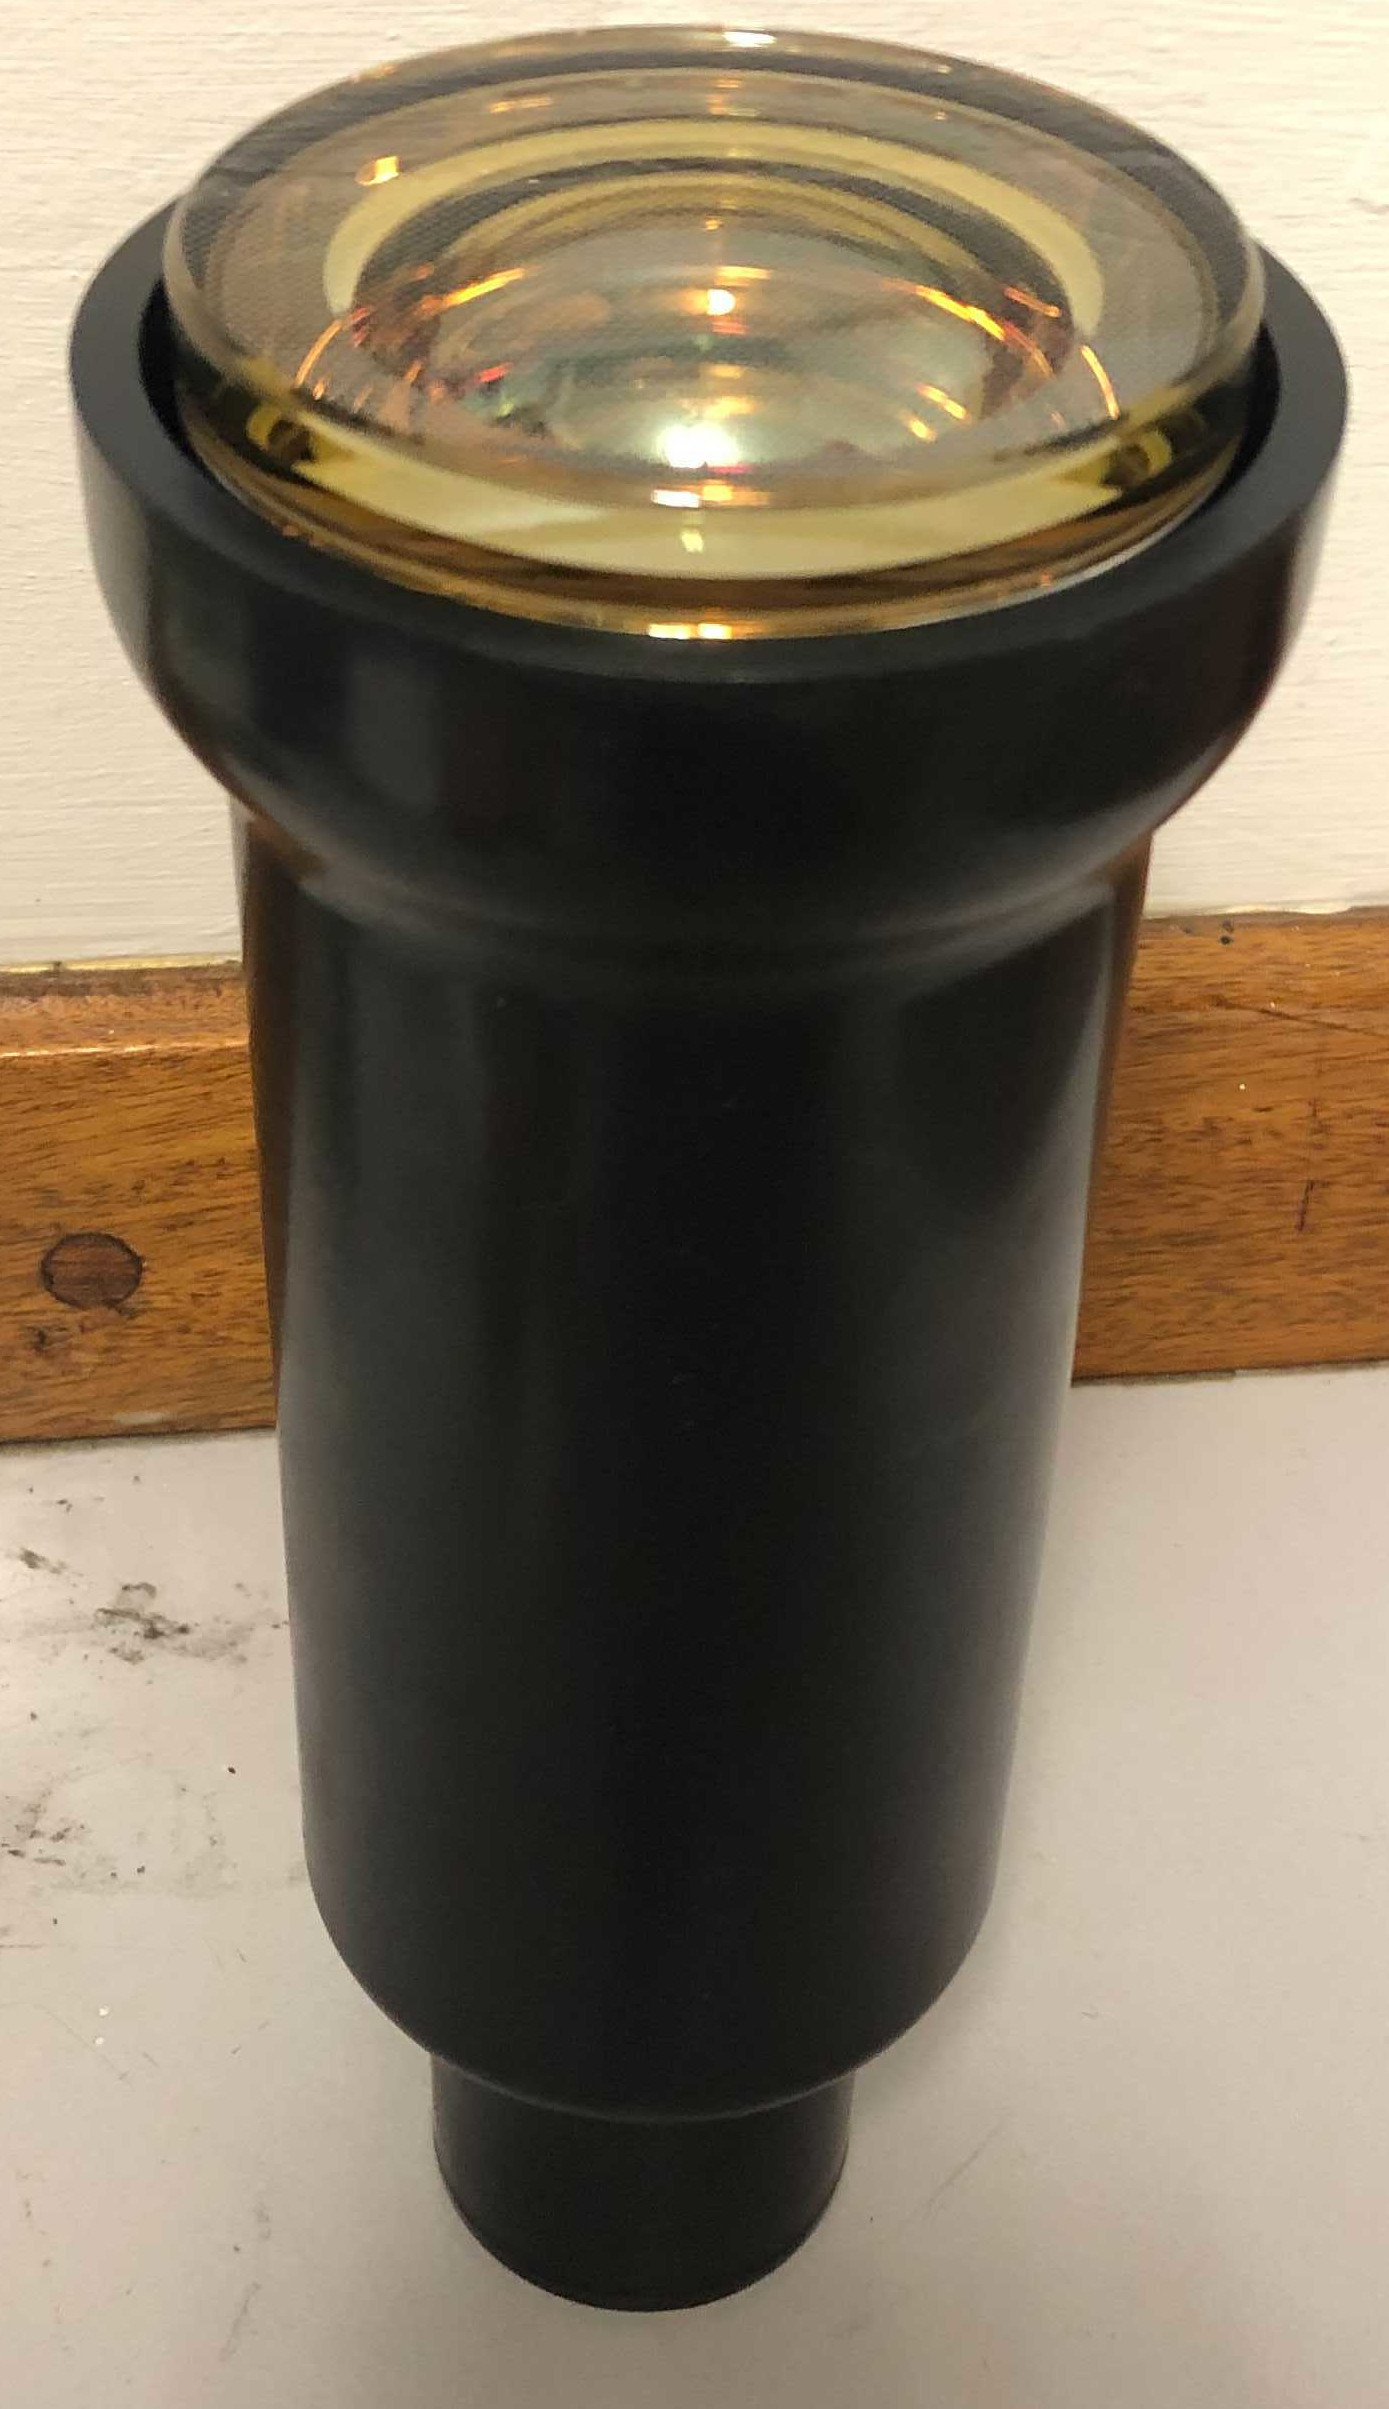
\includegraphics[height=6cm]{diagrams/4-chips/madison_assembly.jpg}%
    }
    \caption[Madison POM PMT assembly.]
    {A Hamamatsu R6091 Madison POM PMT outside (a) and inside its insert (b). The PMT is
        \emph{potted} inside its black PVC insert creating a watertight seal that can withstand the
        \unit{6}{\mathrm{atm}} of water pressure at the bottom of the pit.}
    \label{fig:madison_pmt_assembly}
\end{figure}

\begin{figure} % NIKHEF POM DIAGRAM %
    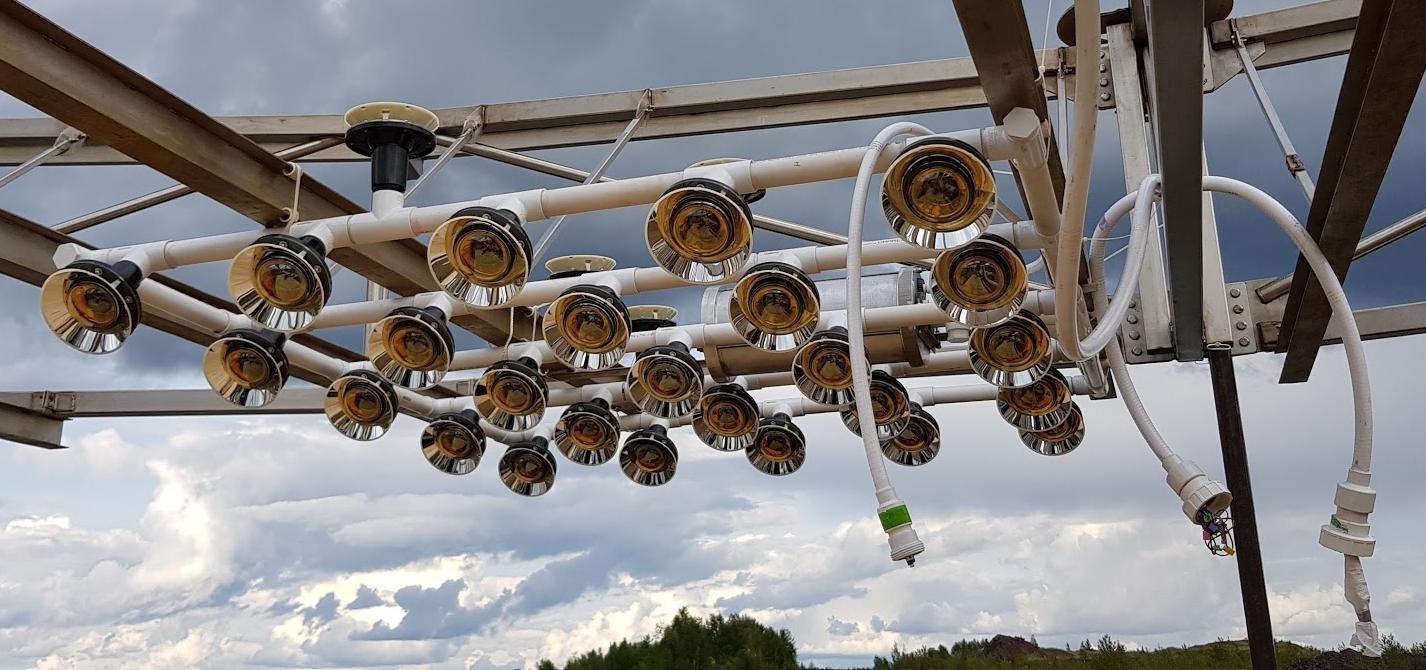
\includegraphics[width=\textwidth]{diagrams/4-chips/single_plane.jpg}
    \caption[Picture of a Nikhef POM.]
    {Picture of a single Nikhef full density POM installed on the top-cap of the \chipsfive
        detector. Both the inward-facing and veto PMTs are visible as well as the aluminium
        electronics container and pigtail whose end is covered in green tape.}
    \label{fig:single_plane}
\end{figure}

The POMs are tiled next to each other on the detector walls, attached to either the stainless
steel \emph{stringers} on the top-cap and bottom-cap, or clipped to the Dyneema cables on the
vertical walls of the \emph{barrel}. As mentioned previously, full high density and high coverage
detector instrumentation is not required for \chips detector modules, due to two main reasons.
Firstly, only highly directional accelerator beam events are to be studied. Therefore, the vast
majority of neutrino interaction Cherenkov radiation is deposited on a relatively small downstream
region of the detector walls. Secondly, beam neutrinos predominantly have multi-$\GeV$ energies,
yielding a relatively large amount of Cherenkov radiation. Therefore, a lower number of PMTs is
required to capture adequate Cherenkov radiation from an interaction.

Consequently, the distribution of the percentage of the detector walls covered by sensitive PMT
surface area (\emph{photocathode coverage}) is optimised to reduce the total number of PMTs. The
detector is split into three distinct regions of PMT photocathode coverage whose boundaries are
roughly defined by their azimuth angle $\phi$ from the centre of the downstream wall (at
$\phi=0^{\circ}$). Firstly, a \emph{full-density} Nikhef POM region in the most downstream
$\phi=\pm75^{\circ}$ region of the detector with a $\sim3\%$ photocathode coverage. Secondly, a
\emph{half-density} Nihkef POM region covering the $\phi=\pm75^{\circ}$ to $\phi=\pm180^{\circ}$
region of the endcaps and the $\phi=\pm75^{\circ}$ to $\phi=\pm140^{\circ}$ region of the barrel
with a $\sim1.5\%$ photocathode coverage. Finally, a \emph{half-density} Madison POM region
covering the $\phi=\pm140^{\circ}$ to $\phi=\pm180^{\circ}$ upstream region of the barrel with a
$\sim0.8\%$ photocathode coverage. Studies have shown that this configuration does not reduce
performance while vastly reducing the number of required PMTs~\cite{blake2016}.

Compared to the $\sim40\%$ uniform photocathode coverage of Super-Kamiokande, the \chipsfive
instrumentation configuration highlights just how significantly different detector design can be
when only studying accelerator beam neutrinos. Of importance to note is that photocathode coverage
in the upstream regions of the detector is still required, even if very low, for cosmic muon and
NC event rejection.

To further help with cosmic muon rejection, the \chipsfive detector module is equipped with a veto
region within the top-cap frame structure. Separated from the main detector volume by a
geomembrane liner, the \unit{1.3}{\mathrm{m}} high region can reject predominantly downward cosmic
muons by detecting the Cherenkov radiation they produce. $324$ \unit{88}{\mathrm{mm}} HZC PMTs are
included within the Nikhef POMs attached to the top-cap facing upwards leading to a veto
photocathode coverage of $\sim0.6\%$. A graphical rendering of all the top-cap POMs is shown in
Fig.~\ref{fig:top_cap}.

\begin{figure} % TOP CAP RENDER DIAGRAM %
    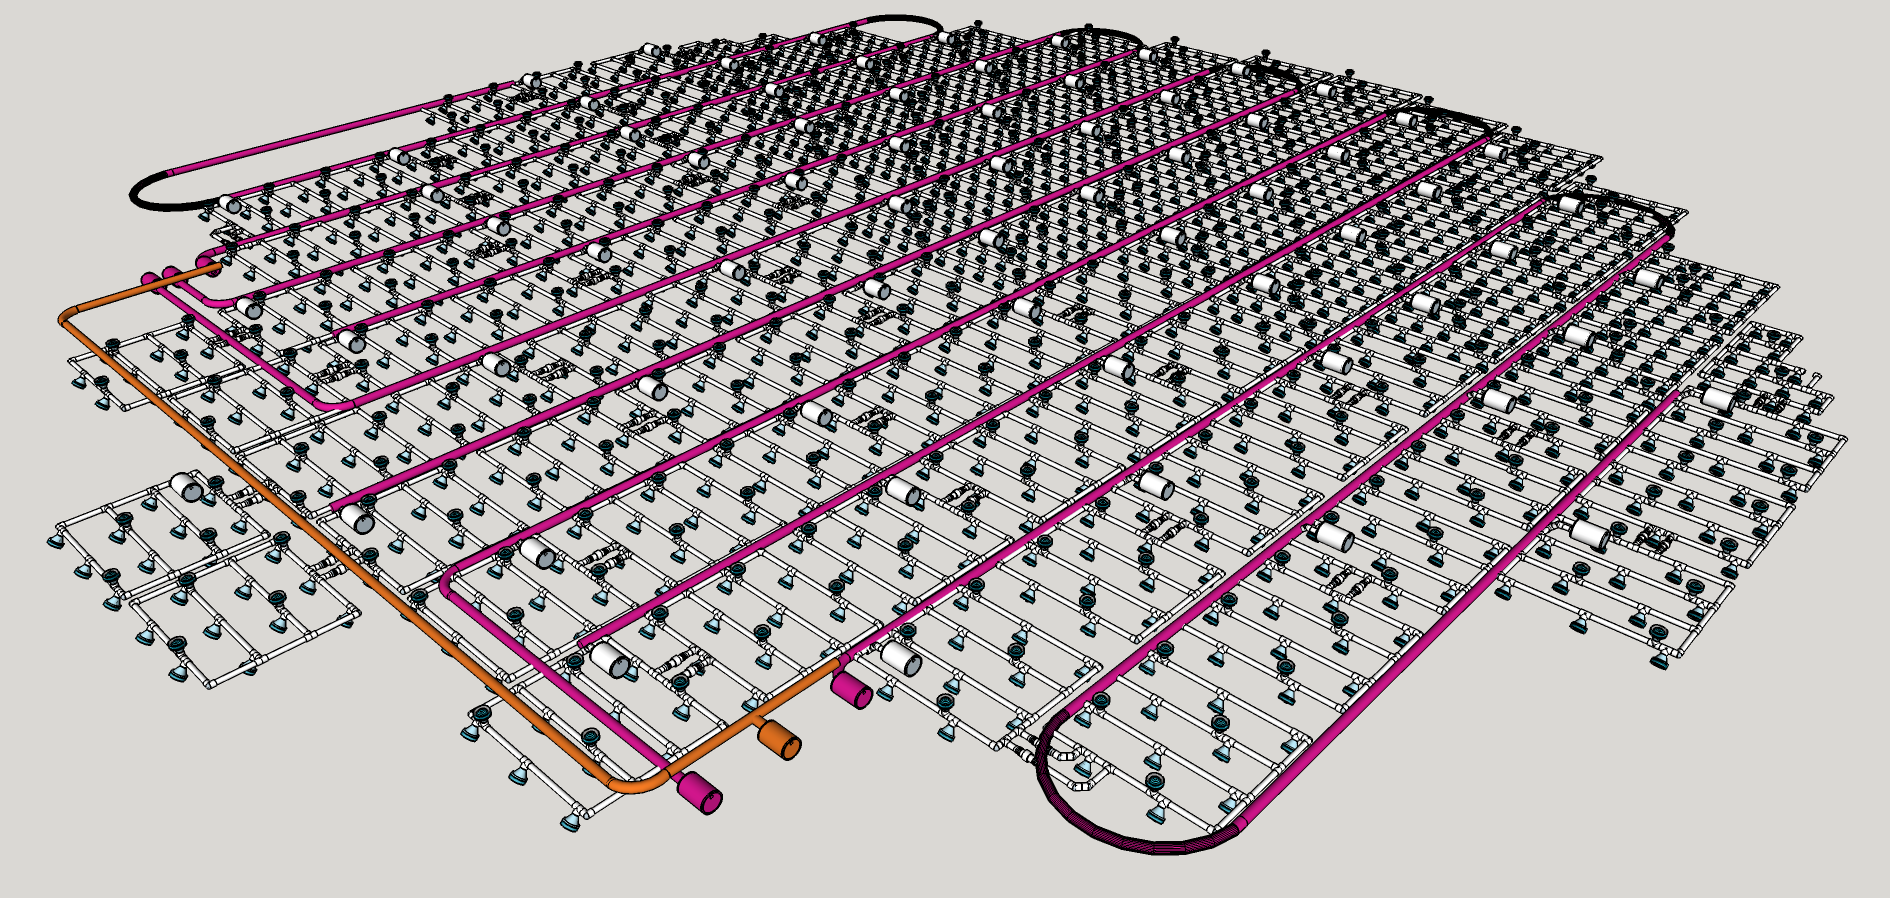
\includegraphics[width=\textwidth]{diagrams/4-chips/top_cap.png}
    \caption[Graphical rendering of the top-cap POMs.]
    {Graphical rendering of the top-cap POMs. Both the different photocathode coverage regions and
        the veto PMTs are visible.}
    \label{fig:top_cap}
\end{figure}

\subsection{Filtration} %%%%%%%%%%%%%%%%%%%%%%%%%%%%%%%%%%%%%%%%%%%%%%%%%%%%%%%%%%%%%%%%%%%%%%%%%%
\label{sec:chips_detector_water} %%%%%%%%%%%%%%%%%%%%%%%%%%%%%%%%%%%%%%%%%%%%%%%%%%%%%%%%%%%%%%%%%

Though surprisingly clear the Wentworth 2W pit water still requires filtration to reach the
required $\sim$\unit{30}{\mathrm{m}} attenuation length of light.

- Though remarkably clear the Wentworth pit water is not clean enough for the detector volume
where we require ~30m attenuation length. Need to pump water, to prevent algae blooms and
bacterial growth and remove particulates which are present in the water to begin with. An
umbilical resting on the pit floor will contain 2 fibres, 2 power cables and 2 flexible pipes for
filtering the internal water on shore. All connected to two shore huts, one for filtering and one
for data acquisition.

- A small positive pressure is kept inside the detector to prevent particulates coming in via and
leaks etc...

\subsection{Construction and deployment} %%%%%%%%%%%%%%%%%%%%%%%%%%%%%%%%%%%%%%%%%%%%%%%%%%%%%%%%%
\label{sec:chips_detector_deployment} %%%%%%%%%%%%%%%%%%%%%%%%%%%%%%%%%%%%%%%%%%%%%%%%%%%%%%%%%%%%

- How it can grow if needed - buoyant top cap anchored to the bottom one, which when fully
deployed will rest on the bottom of the pit.

\subsection{Current status} %%%%%%%%%%%%%%%%%%%%%%%%%%%%%%%%%%%%%%%%%%%%%%%%%%%%%%%%%%%%%%%%%%%%%%
\label{sec:chips_detector_status} %%%%%%%%%%%%%%%%%%%%%%%%%%%%%%%%%%%%%%%%%%%%%%%%%%%%%%%%%%%%%%%%

- No liner between veto and main volume!
- In the summer of 2018 and 2019 work on deploying \chips proceeded. Unforeseen hehe!!

This highlights one of the clear advantages of the \chips concept. No physical structure is
required on the barrel of the detector. Alongside the easier deployment discussed in
Section~\ref{sec:chips_detector_deployment} and the significantly simplified engineering, this is
the key reason as to why the \chips concept uses cylindrical rather than spherical detector
modules.

\begin{figure} % WORK DIAGRAM %
    \centering
    \subcaptionbox{gwgw}{%
        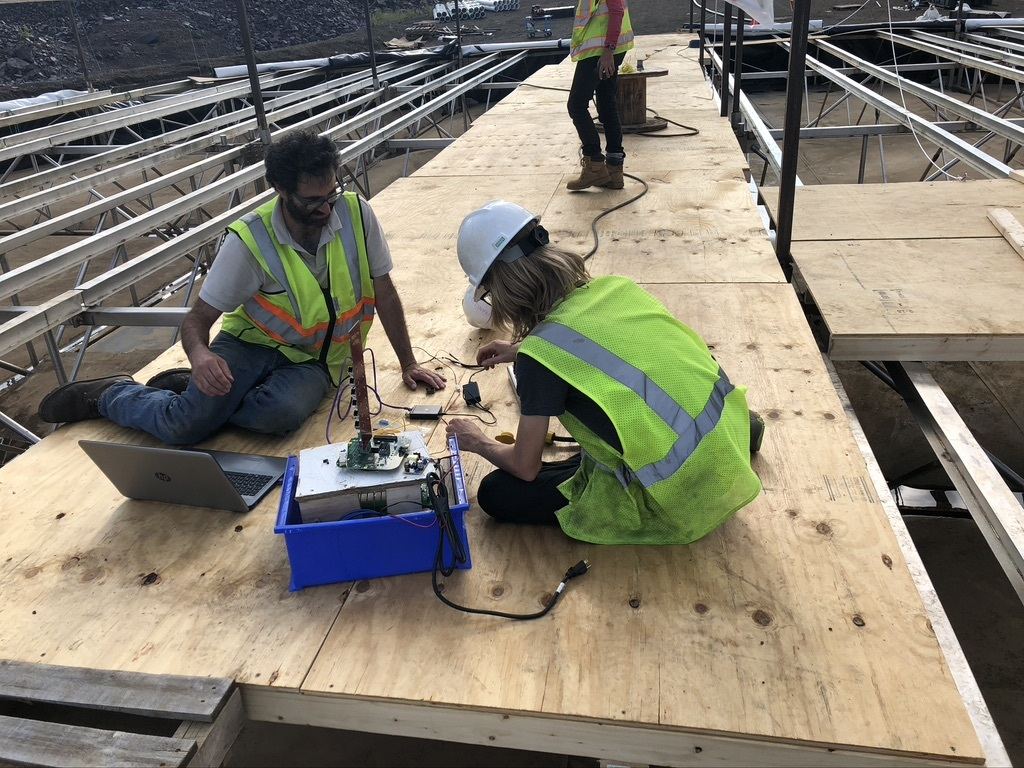
\includegraphics[height=5.5cm]{diagrams/4-chips/work1.jpeg}%
    }
    \quad
    \subcaptionbox{asgag}{%
        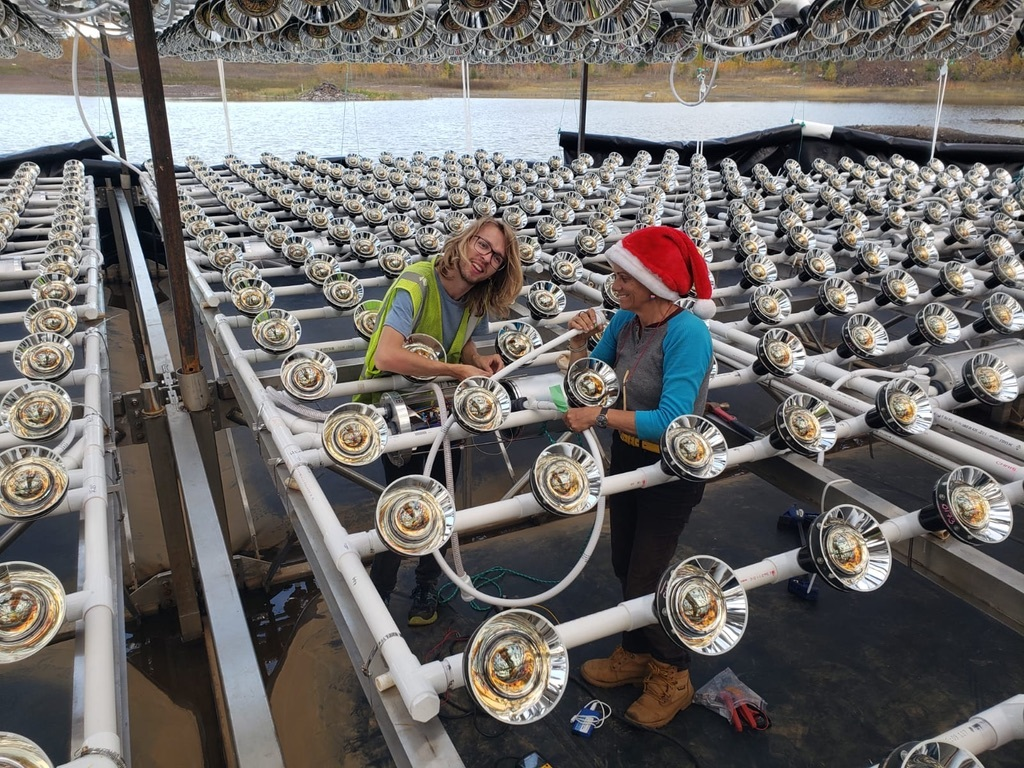
\includegraphics[height=5.5cm]{diagrams/4-chips/work2.jpeg}%
    }
    \caption[afaga]
    {afag}
    \label{fig:work}
\end{figure}

\begin{figure} % PANORAMA DIAGRAM %
    \includegraphics[width=\textwidth]{diagrams/4-chips/pan_1.jpeg}
    \caption[Panorama of the inside of \chipsfive just before deployment.]
    {Panorama of the inside of \chipsfive just before deployment. The six deployed Madison POMs
        are visible in the foreground on the bottom endcap. Additionally, the flexible tube manifolds
        can be seen connecting each POM to the higher level DAQ electronics.}
    \label{fig:pan_1}
\end{figure}

\section{Monte Carlo event generation and simulation} %%%%%%%%%%%%%%%%%%%%%%%%%%%%%%%%%%%%%%%%%%%%
\label{sec:chips_monte_carlo} %%%%%%%%%%%%%%%%%%%%%%%%%%%%%%%%%%%%%%%%%%%%%%%%%%%%%%%%%%%%%%%%%%%%

- Indispensable tool in particle physics, during the design and data analysis stages. Allows for
optimisation studies, testing of event reconstruction techniques and the study of potential
physics sensitivity.
- Useful MC simulation will provide output matching observables in a real detector. For full
analysis simulations need to be validated fully to make sure they approximate reality well enough.

\subsection{Beam event generation} %%%%%%%%%%%%%%%%%%%%%%%%%%%%%%%%%%%%%%%%%%%%%%%%%%%%%%%%%%%%%%%
\label{sec:chips_monte_carlo_beam} %%%%%%%%%%%%%%%%%%%%%%%%%%%%%%%%%%%%%%%%%%%%%%%%%%%%%%%%%%%%%%%

The expected energy spectrum (flux) of neutrinos at the \chipsfive detector location is generated
using the existing beam simulation written for the \numi beam experiments, and shown in
Fig.~\ref{fig:flux}. As the $\nu_{\tau}$ component is negligible, it is not predicted by the beam
simulation and ignored. Using the generated fluxes as input the GENIE neutrino event generator
(version 3.0.6)~\cite{andreopoulos2009, andreopoulos2015} is used to generate beam neutrino
events. Default cross-sections on water provided by GENIE are used. All initial, intermediate, and
final state particle tracks for each event are stored as output in a NUANCE formatted file for use
in the detector simulation. Note that unoscillated fluxes are used such that analyses samples must
be weighted to match the desired oscillated neutrino composition.

\begin{figure} % CHIPS FLUX DIAGRAM %
    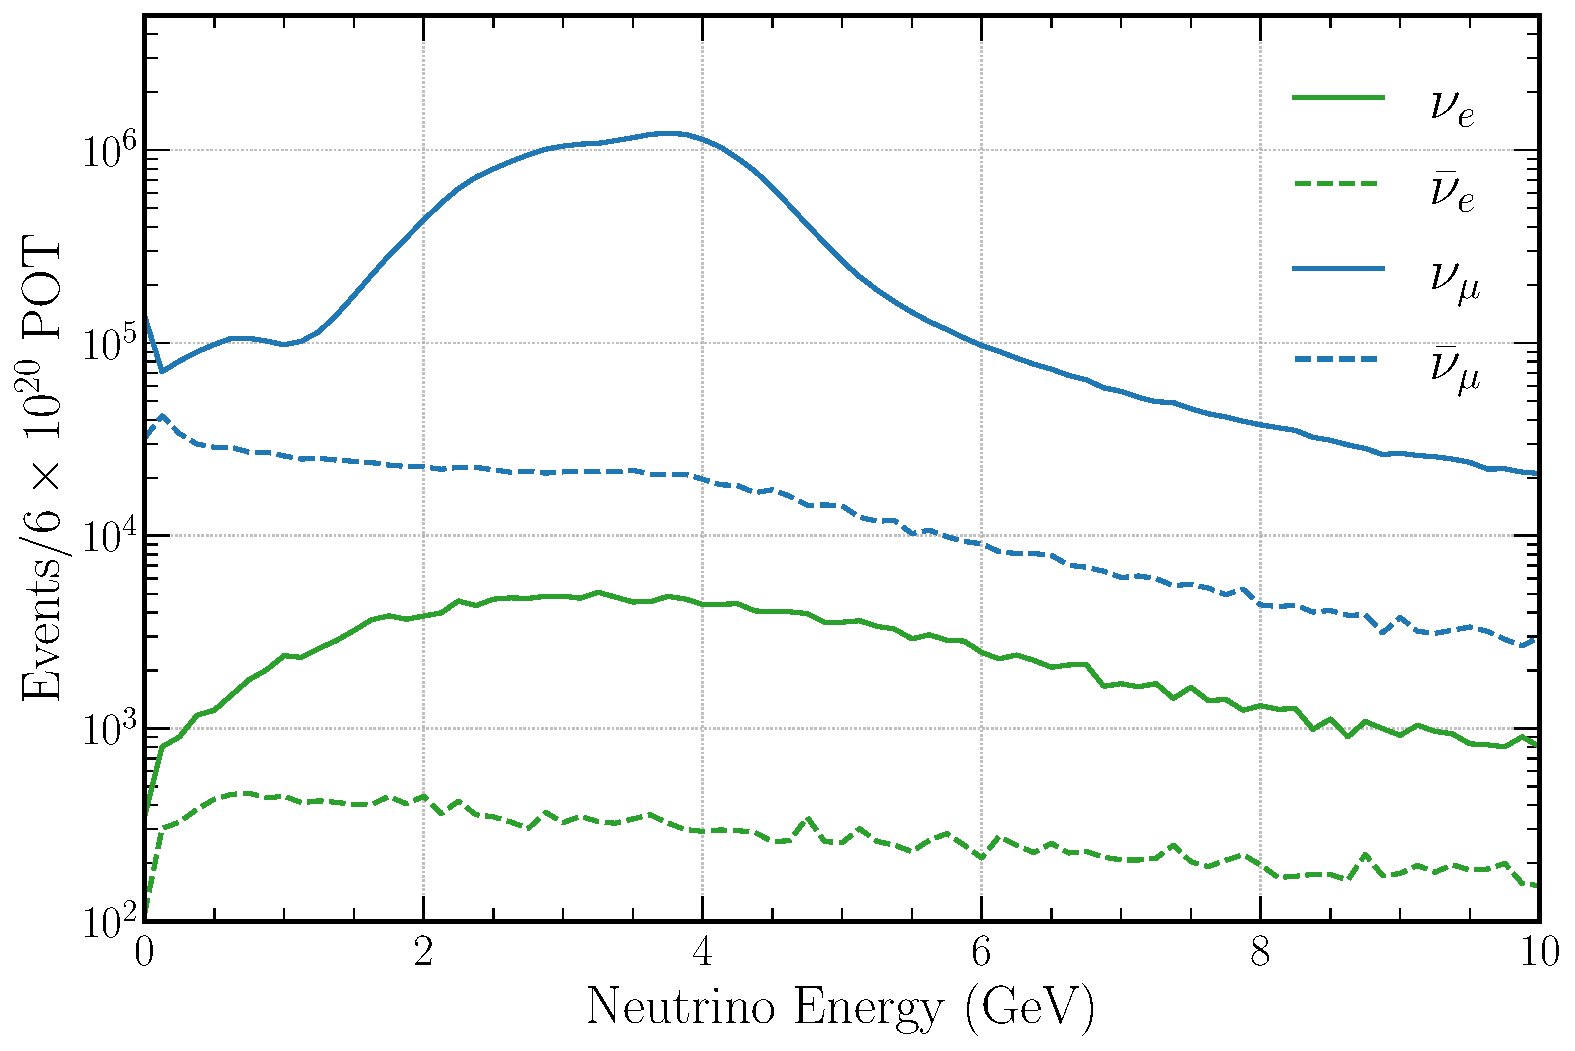
\includegraphics[width=0.8\textwidth]{diagrams/4-chips/flux.pdf}
    \caption[\numi neutrino flux at CHIPS.]
    {The neutrino mode (forward horn current) \numi beam neutrino energy spectrum at the
        \chipsfive detector module location. Shown are the separate contributions from the
        different neutrino types and signs. No cross-sections or oscillations have been applied.}
    \label{fig:flux}
\end{figure}

\subsection{Cosmic event generation} %%%%%%%%%%%%%%%%%%%%%%%%%%%%%%%%%%%%%%%%%%%%%%%%%%%%%%%%%%%%%
\label{sec:chips_monte_carlo_cosmic} %%%%%%%%%%%%%%%%%%%%%%%%%%%%%%%%%%%%%%%%%%%%%%%%%%%%%%%%%%%%%

The Cosmic-Ray Shower Library (CRY)~\cite{hagmann2012_1, hagmann2012_2} is used for cosmic ray
event generation. Both the solar cycle and Earth's geomagnetic field are taken into account, with
the \chipsfive latitude and deployment date (1st November 2019) used as input. Single muons are
generated at \emph{sea level} by CRY within a
\unit{1000}{\mathrm{m}}$\times$\unit{1000}{\mathrm{m}} area, with the detector at the centre.

Assuming a \chipsfive overburden of \unit{50}{\mathrm{m}} and a \unit{2.2}{\MeV/\mathrm{cm}^{2}}
muon energy loss in water as suggested in Ref.~\cite{klimushin2001} the muon parameters are
updated to estimate their values \unit{1}{\mathrm{m}} above the top of the detector. All muons
whose path does not cross the detector volume or do not have sufficient energy are discarded. All
accepted muon tracks are stored as output in a NUANCE formatted file for use in the detector
simulation~\cite{chipsgen2020}.

Extensive studies have looked at the likely cosmic rate for \chips detector modules at different
water overburden depths~\cite{son2013}. In this work, the fits shown in Fig.~\ref{fig:cosmic_rate}
for a cylindrical detector of both height and diameter \unit{24}{\mathrm{m}} are used to estimate
a cosmic muon rate of \unit{11.8}{\mathrm{KHz}} at \unit{50}{\mathrm{m}} of overburden for
\chipsfive. For the \unit{10}{\mu\mathrm{s}} long \numi beam spill occurring every
\unit{1.33}{\mathrm{s}} this gives an in spill cosmic rate of $\sim2.1$ million events per year
and an in spill occupancy of 9\%. Considering a typical event takes $\sim100\mathrm{ns}$ to
unfold, there is approximately a 0.3\% chance that any beam event overlaps with a cosmic muon.
This low coincidence shows just how powerful using a short beam spill is at reducing the cosmic
background.

\begin{figure} % COSMIC RATE DIAGRAM %
    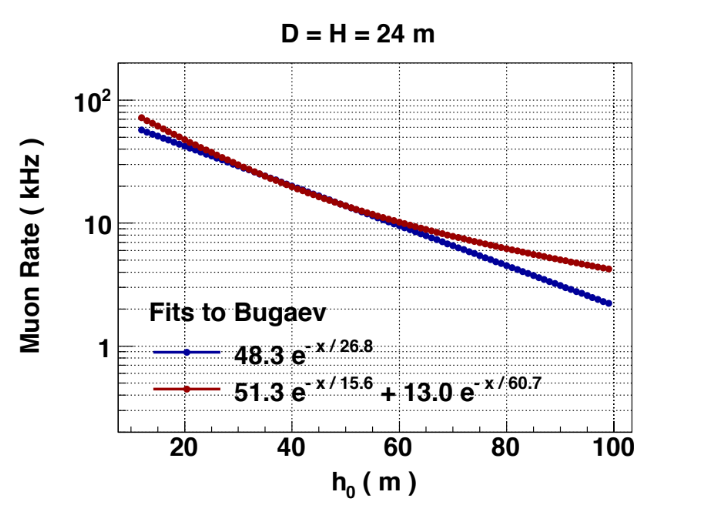
\includegraphics[width=0.6\textwidth]{diagrams/4-chips/cosmic_rate.png}
    \caption[Expected \chipsfive cosmic muon rate as a function of depth.]
    {Expected cosmic muon rate as a function of water overburden depth for a \unit{24}{\mathrm{m}}
        high and \unit{24}{\mathrm{m}} wide \chips detector module. Shown are fits made to the work
        originally conducted in Ref.~\cite{bugaev1998}. Figure taken from Ref.~\cite{son2013}.}
    \label{fig:cosmic_rate}
\end{figure}

\subsection{Detector simulation} %%%%%%%%%%%%%%%%%%%%%%%%%%%%%%%%%%%%%%%%%%%%%%%%%%%%%%%%%%%%%%%%%
\label{sec:chips_monte_carlo_sim} %%%%%%%%%%%%%%%%%%%%%%%%%%%%%%%%%%%%%%%%%%%%%%%%%%%%%%%%%%%%%%%%

The detector simulation uses the WCSim water Cherenkov simulation package~\cite{wcsim2020} built
on top of the Geant4 simulation framework~\cite{agostinelli2003, allison2006, Allison2016}.
Originally developed to simulate possible water Cherenkov detectors in the LBNE beam (now LBNF),
WCSim is now used more widely in the field for generic water Cherenkov detectors. WCSim has been
heavily modified for the \chips project to allow for generic water Cherenkov detector geometries
to be easily loaded at runtime via a series of simple XML configuration files. These changes allow
for a broad range of detector geometries to be quickly considered without recompilation of the
code.

To represent \chips detector modules, the simulation builds an n-sided, regular polygonal prism
consisting of two endcaps separated by a barrel. The prism is filled with water and lined with a
low reflectivity \emph{blacksheet}. The geometry is separated into \emph{regions} within both the
barrel and endcaps, defined either by a list of barrel sides or an opening angle respectively.
Each region is filled with a unique base unit of geometry known as the \emph{unit cell} as shown
in Fig.~\ref{fig:sim_geom}.

The unit cell defines a pattern of any number of PMTs, as well as their relative positions and in
which direction they face. The final geometry is built by tiling each of the defined regions with
their respective unit cell scaled to match the required regional photocathode coverage. Note that
although exact PMT positions are not used in this procedure, a given configuration always
generates the same geometry (it is deterministic). In this work the \chipsfive geometry is
generated with 28 sides regions matching the angles and photocathode coverage outlined in
Section.~\ref{sec:chips_detector_instrumentation}.

\begin{figure} % SIMULATION GEOM DIAGRAM %
    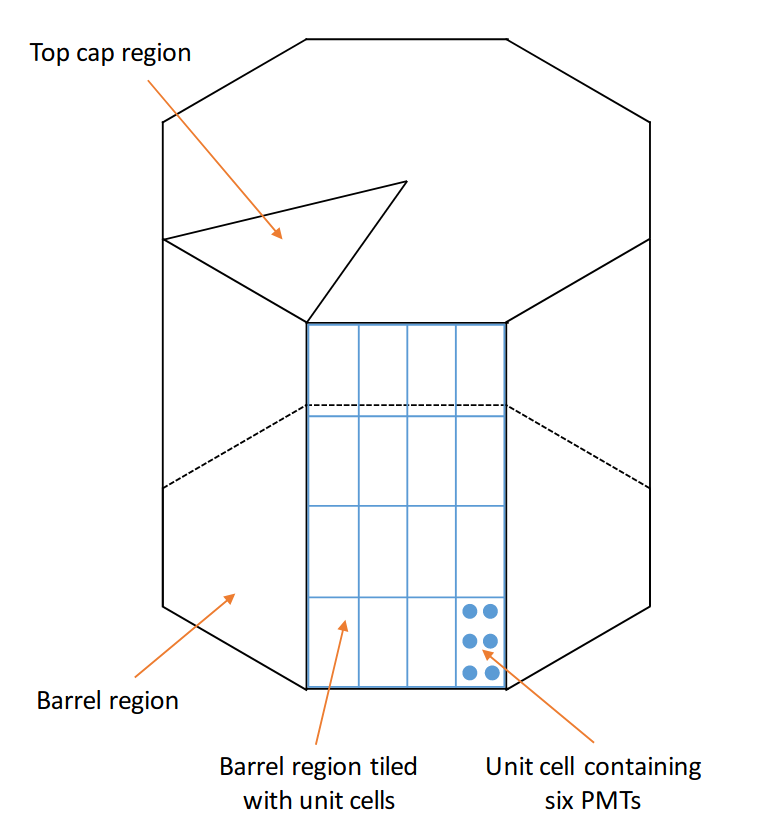
\includegraphics[width=0.6\textwidth]{diagrams/4-chips/sim_geom.png}
    \caption[Illustrative diagram of a WCSim detector geometry.]
    {Illustrative diagram of a WCSim detector geometry, showing the shape, endcap and barrel
        regions, tiled unit cells and PMTs within a unit cell. Figure taken from
        Ref.~\cite{blake2016}.}
    \label{fig:sim_geom}
\end{figure}

The geometry shape, regions, and unit cells are defined in a configuration file. Additionally, a
file for PMT definitions containing their shape, time resolution, and quantum efficiency is
defined. Light cones are described by a list of radial profile points in a further file. Although
the underlying Geant4 material properties are mostly hardcoded (taken from the Super-Kamiokande
simulation) they can be scaled by values within yet another configuration file. This file controls
the water absorption and scattering (Rayleigh and Mie) lengths, and both the blacksheet and PMT
glass reflectivity. In this work an attenuation length of \unit{50}{\mathrm{m}} at
\unit{405}{\mathrm{nm}} is used with negligible scattering, the blacksheet reflectivity is set to
be 4\% and the PMT glass reflectivity 24\%.

A veto volume can also be defined. The veto is built as either a concentric shell around the whole
inner volume with a given thickness or solely above the top-cap with a given height. Any PMTs
defined as facing outwards within a unit cell look into the veto volume instead of the inner
volume.

Once the full generation of the runtime Geant4 geometry is complete, the final state tracks for
each successive event to be simulated are loaded from either the beam or cosmic event generator
NUANCE files. Beam event vertices are randomly placed within the inner detector volume, while
cosmic vertices are kept at \unit{1}{\mathrm{m}} above the detector volume. WCSim then simulates
the passage of all particles through the detector materials, with interactions, decays, and
Cherenkov emission also considered.

Whenever a photon is calculated to have hit the photocathode of a PMT an angular dependent
acceptance efficiency is applied to see if it it is recorded. If accepted all hits within
\unit{200}{\mathrm{ns}} windows are grouped together to output a single `recorded' PMT hit, with
the smeared first photon hit time used as the recorded hit time. 

Whenever a photon is calculated to have hit the photocathode of a PMT a digitisation simulation is
used to convert the true photon hits into a `recorded' charge in photoelectrons. All hits within
\unit{200}{\mathrm{ns}} windows are grouped together for each recorded hit, with the first smeared
photon hit time used. A method similar the that used in the Super-Kamiokande simulation is used to
calculate the overall charge. For each photon a single photoelectron charge distribution is probed
and the combined sum returned. By sampling this procedure many times the probability distribution
given a number of input photons is given in Fig.~\ref{fig:digitisation}.

\begin{figure} % DIGI DIAGRAM %
    \centering
    \subcaptionbox{\label{fig:digi_method}}{%
        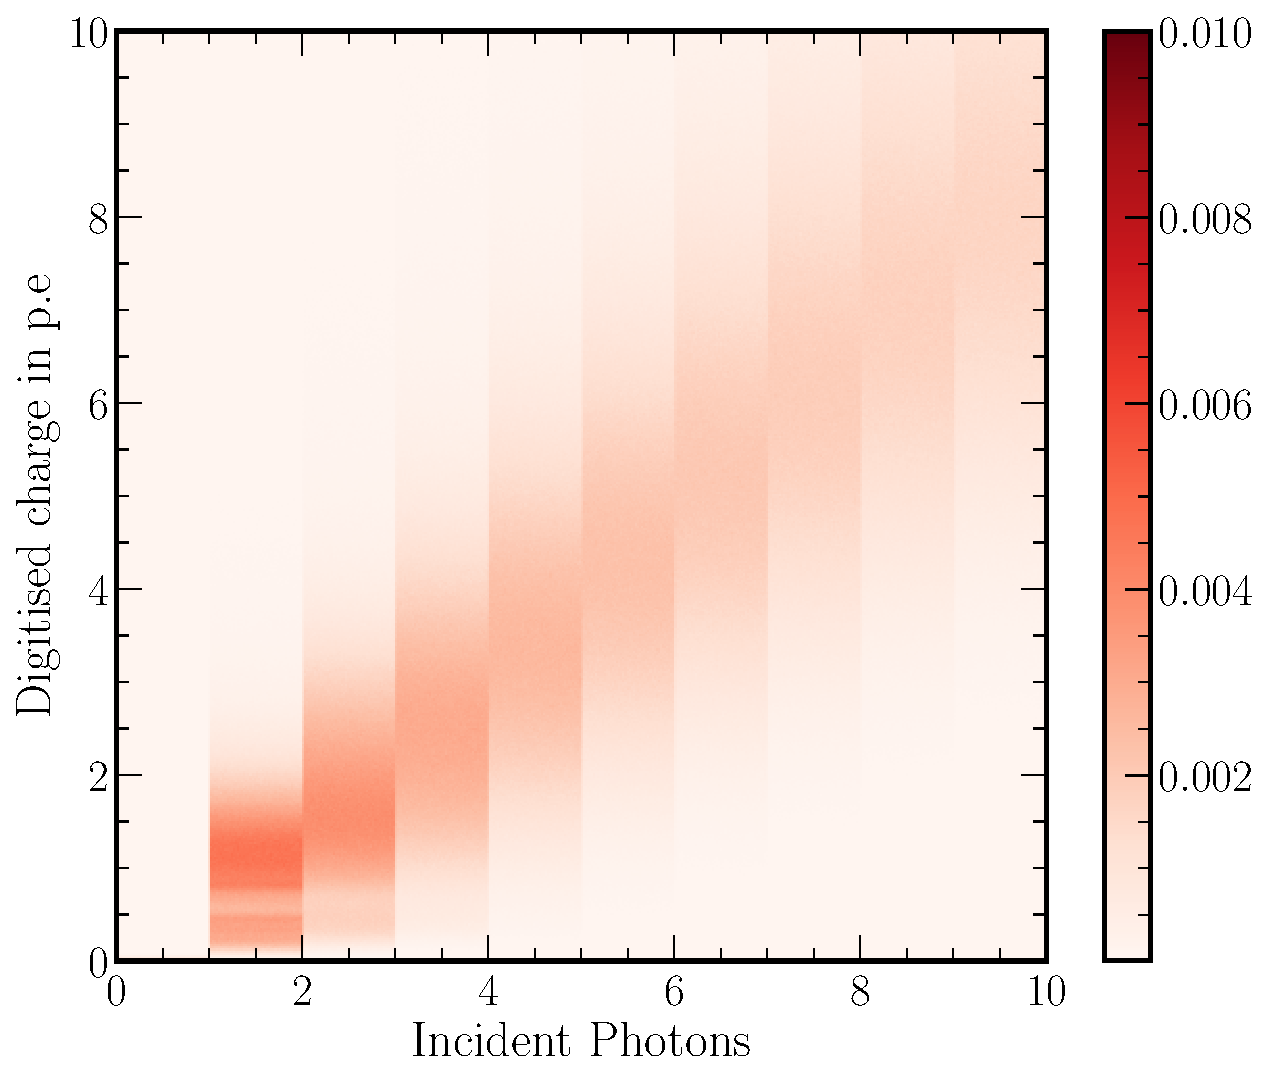
\includegraphics[height=6cm]{diagrams/4-chips/digi_method.pdf}%
    }
    \quad
    \subcaptionbox{\label{fig:digi_likelihood}}{%
        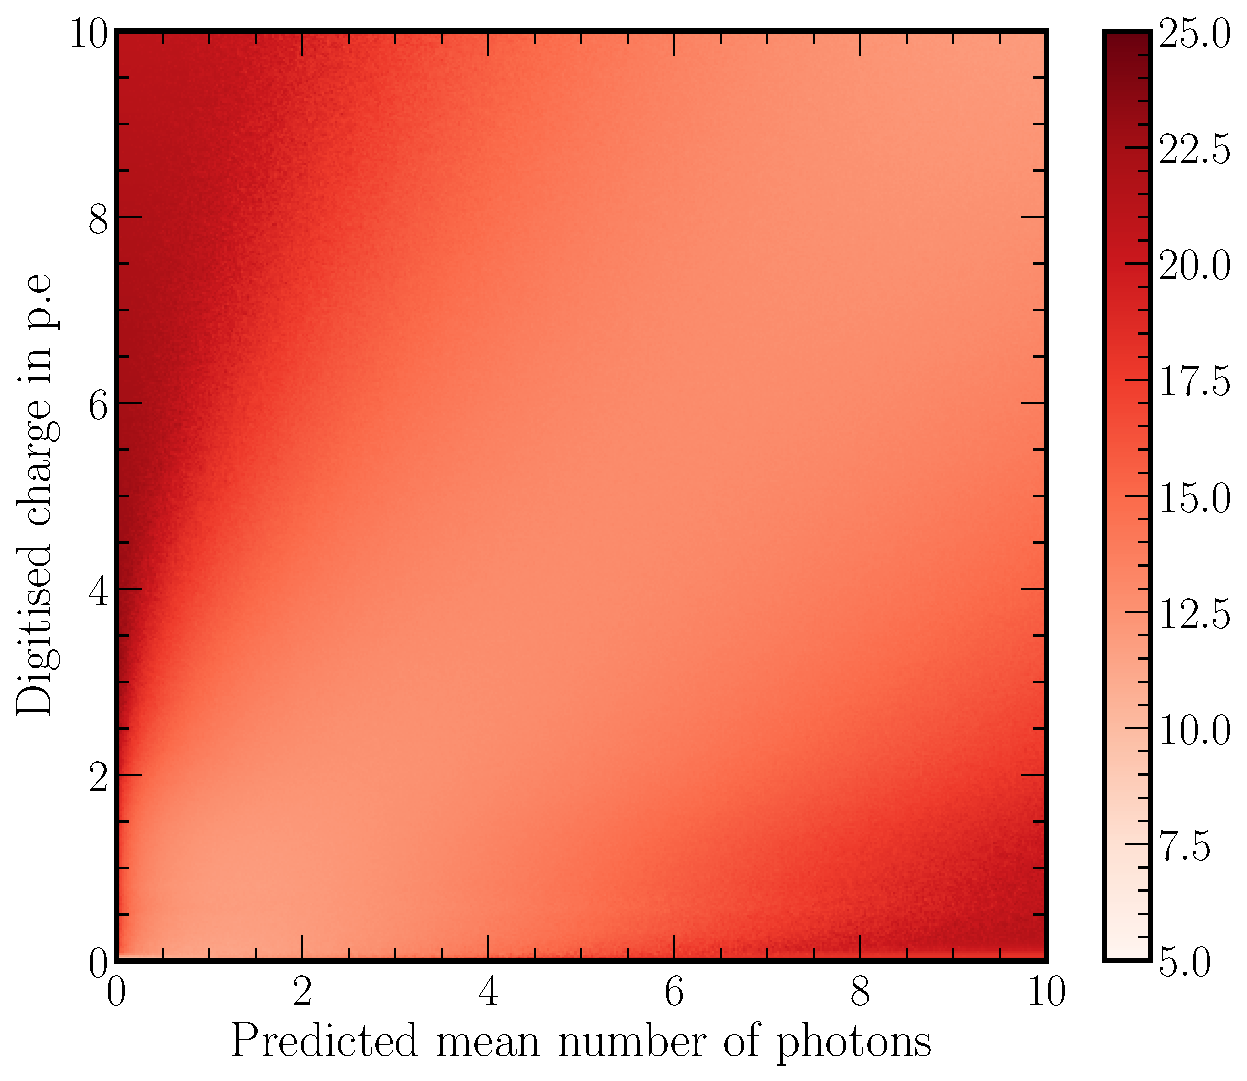
\includegraphics[height=6cm]{diagrams/4-chips/digi_likelihood.pdf}%
    }
    \caption[Detector simulation PMT digitisation function.]
    {The detector simulation digitisation probability function (a) used for the Nikhef

        (a) Digitisation probability function used within the simulation to convert incident photons
        to a measured digitised charge. (b) Likelihood of a measured digitised charge being caused
        by a number of photons incident on a PMT.}
    \label{fig:digitisation}
\end{figure}

- Angular efficiency
- default Geant4 physics list is used (QGSP\_BIC\_HP).
- The digitisation function could definitely be improved.
- All hits are recorded as output!!!

\begin{figure} % SIMULATED EVENT DISPLAY DIAGRAM %
    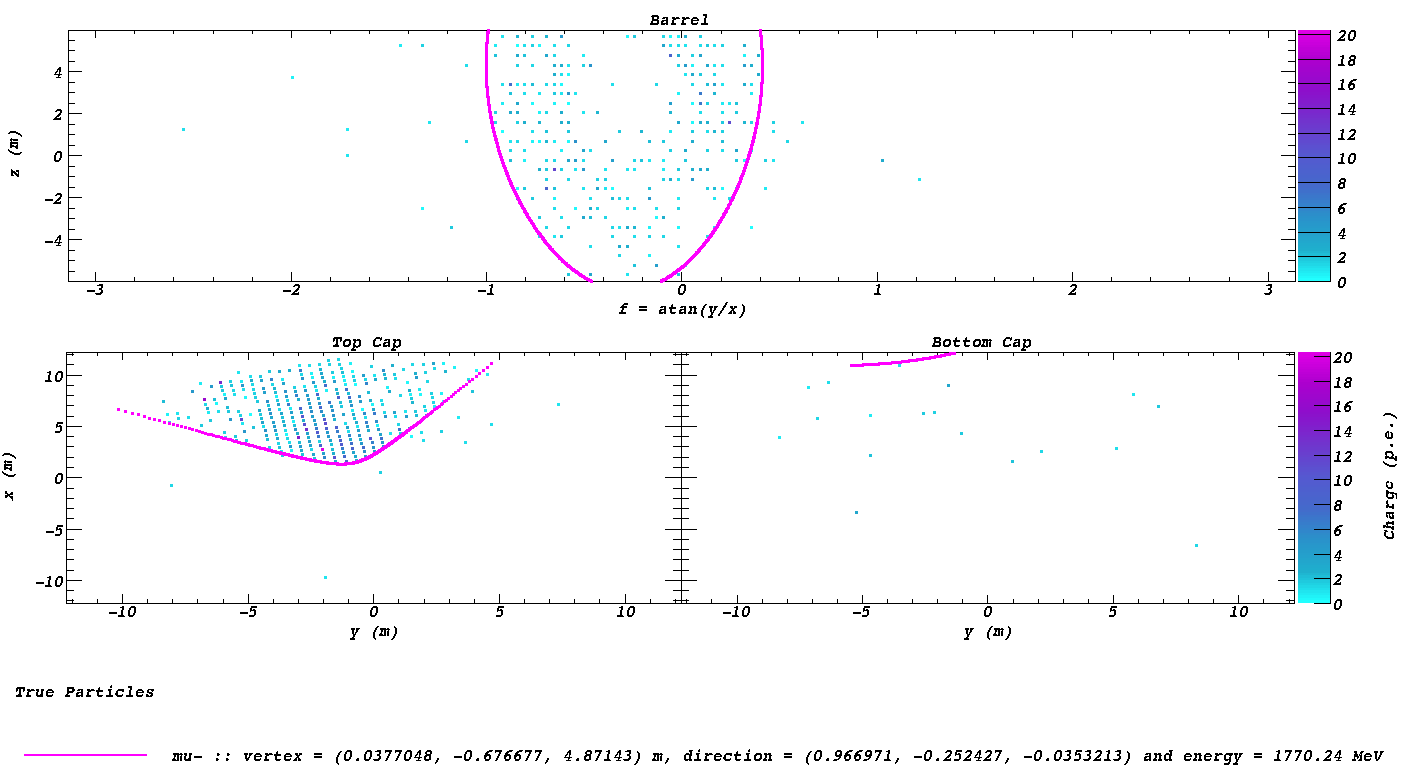
\includegraphics[width=\textwidth]{diagrams/4-chips/sim_event.png}
    \caption[sim event short]
    {Event display of a simulated CC $\nu_{\mu}$ quasi-elastic event with a single muon in the
        final state of energy \unit{1.77}{\GeV}. The display shows both the unrolled barrel of the
        \chipsfive detector as well the two endcaps. Every coloured entry represents a hit PMT
        with the color indicating the total photoelectrons (charge) collected. The pink ring is a
        projection of the true Cherenkov light cone associated with the muon track from the
        interaction vertex.}
    \label{fig:sim_event}
\end{figure}

%%%%%%%%%%%%%%%%%%%%%%%%%%
- These short spills are essential for \chips and other experiments in rejecting the massive
cosmic ray background. As all events outside the expected beam spill window at the detector can be
rejected.
- Only single cosmic muons are considered for simplicity, future work should also consider
electrons, pions and multiple cosmic muons at the same time.

    \chapter{Data acquisition for CHIPS} %%%%%%%%%%%%%%%%%%%%%%%%%%%%%%%%%%%%%%%%%%%%%%%%%%%%%%%%%%%%%
\label{chap:daq} %%%%%%%%%%%%%%%%%%%%%%%%%%%%%%%%%%%%%%%%%%%%%%%%%%%%%%%%%%%%%%%%%%%%%%%%%%%%%%%%%

The primary task of any Data Acquisition system is the processing of low-level signals measuring
real-world physics and their transfer to permanent storage for further analysis. Commonly, this
procedure also includes decision making as to whether the signal is deemed interesting enough to
record, known as a \emph{trigger}. Both these tasks can make DAQ systems incredibly complex,
especially when they must operate in an efficient and resilient manner for vast amounts of data in
real-time, while also providing detector control and monitoring.

In the context of the \chips project, the DAQ system records all PMT hits, timestamps them using a
common clock, and transfers them out of the detector to a central processing node. This node then
applies a trigger to select hits that fall within the interesting \numi beam spill time window,
before the selected hits are sliced into events and moved to permanent storage for further
analysis. Alongside these processes, the DAQ system also configures the detector and provides data
quality and detector component monitoring.

Although relatively simple when compared to the incredibly complex and time-pressured DAQ systems
of the LHC experiments, the DAQ system developed for the \chips project introduces some novel
approaches to solve the unique constraints of the \chips concept. Namely, deployment within a body
of water and a limited resource budget. In this chapter, the DAQ system for \chips as applied to
the \chipsfive prototype detector module is described alongside highlighting any novel approaches.
The description is presented in two broad categories, hardware and software, with a short
description of the timing system beforehand.

\section{White Rabbit timing} %%%%%%%%%%%%%%%%%%%%%%%%%%%%%%%%%%%%%%%%%%%%%%%%%%%%%%%%%%%%%%%%%%%%
\label{sec:daq_timing} %%%%%%%%%%%%%%%%%%%%%%%%%%%%%%%%%%%%%%%%%%%%%%%%%%%%%%%%%%%%%%%%%%%%%%%%%%%

To ensure PMT hit times are synchronised throughout \chips detectors, a common clock must be
shared across all timestamping electronics. For this purpose, \chips uses a \emph{White Rabbit}
(WR) network~\cite{lipinski2011}. Initially developed at CERN, the open-source WR project provides
an ethernet-based time distribution network with sub-nanosecond synchronisation accuracy between
nodes. By using two-way exchanges of WR messages, precise adjustment of individual node clock
phases and offsets is possible across thousands of devices, separated by tens of kilometres. All
of this is achieved in parallel with a standard data transfer network capable of
\unit{1}{\text{Gb}} speeds.

All nodes are synchronised to the clock of a \emph{GrandMaster} node, typically a WR
\emph{switch}, the most common WR hardware component. As input, the switch receives an IRIG-B
(Inter-Range Instrumentation Group timecode B) and a \unit{10}{\text{MHz}} signal from a GPS
disciplined oscillator. These inputs allow for synchronisation of the GrandMaster clock to
International Atomic Time (TAI). As \chips detector modules require synchronisation to accelerator
clocks many hundreds of kilometres away to determine the arrival time of beam spills, the GPS
disciplined timing is particularly important.

WR hardware is commercially available from many vendors. Within \chipsfive, two WR devices are
used for time synchronisation and data transfer, both shown in Fig.~\ref{fig:wr_electronics}.
Firstly, a compact version of the standard WR switch~\cite{wrswitch2020}, specially developed for
the \chips project at Nikhef~\cite{wrchromium2020}. Secondly, a WR-LEN (Lite Embedded Node) from
Seven Solutions~\cite{wrlen2020}. 

\begin{figure} % WHITE-RABBIT COMPONENTS DIAGRAM %
    \centering
    \subcaptionbox{White Rabbit switch}{%
        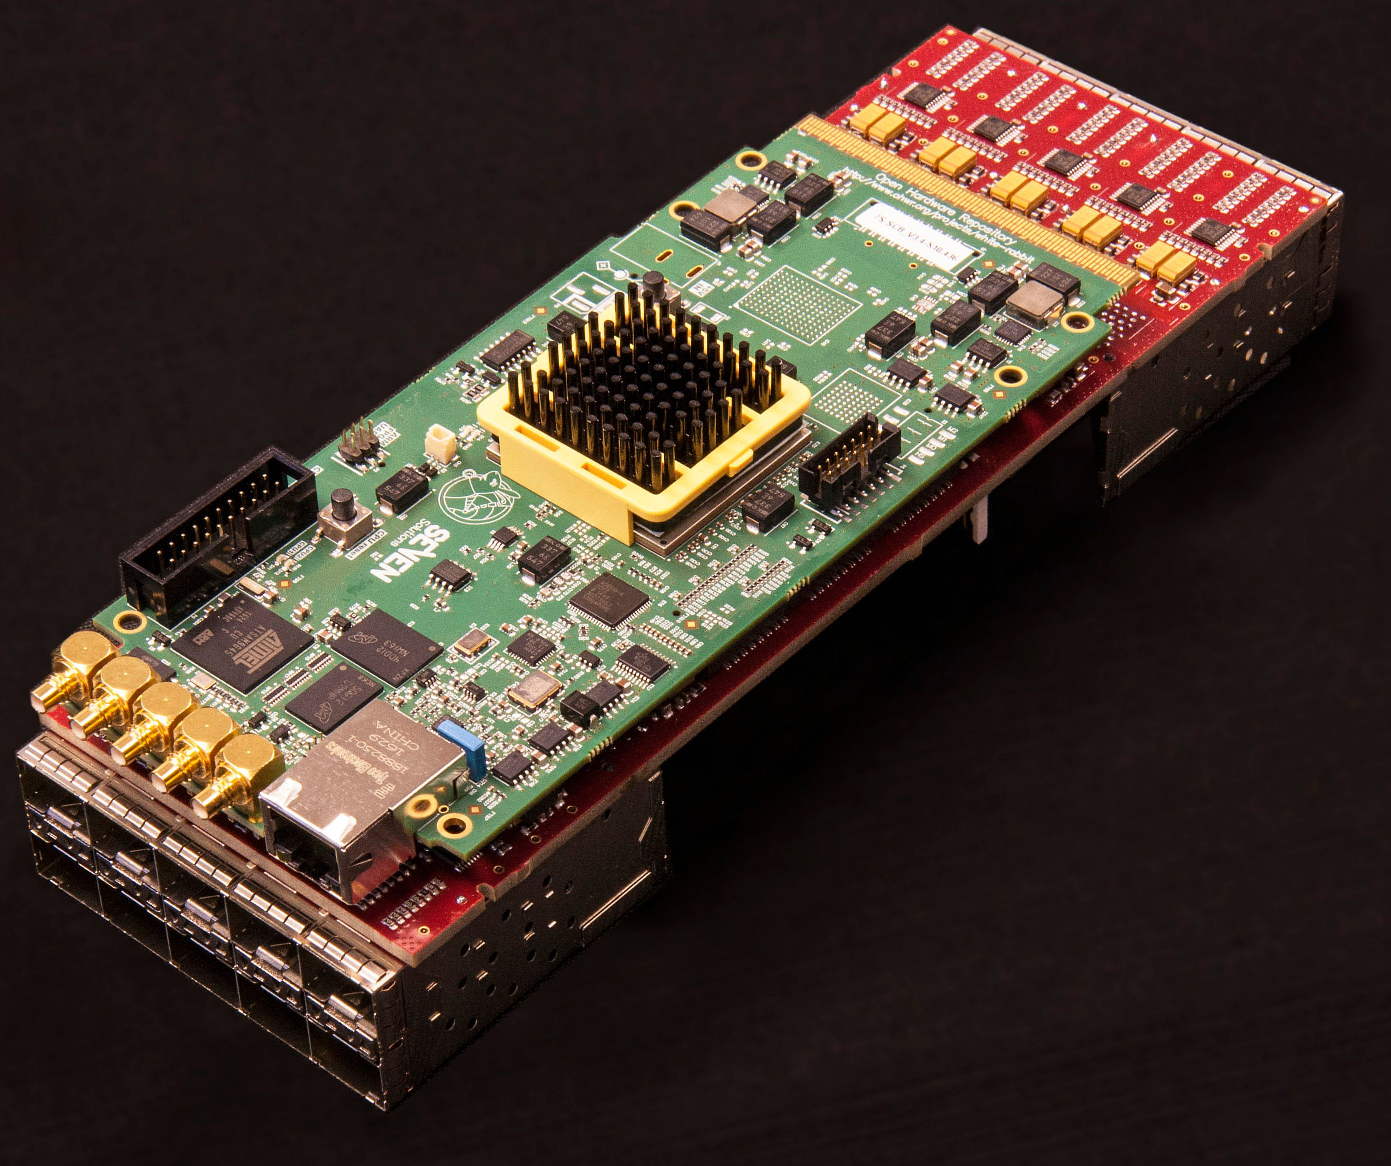
\includegraphics[height=6cm]{diagrams/5-daq/wr_switch.pdf}%
    }
    \quad
    \subcaptionbox{White Rabbit LEN}{%
        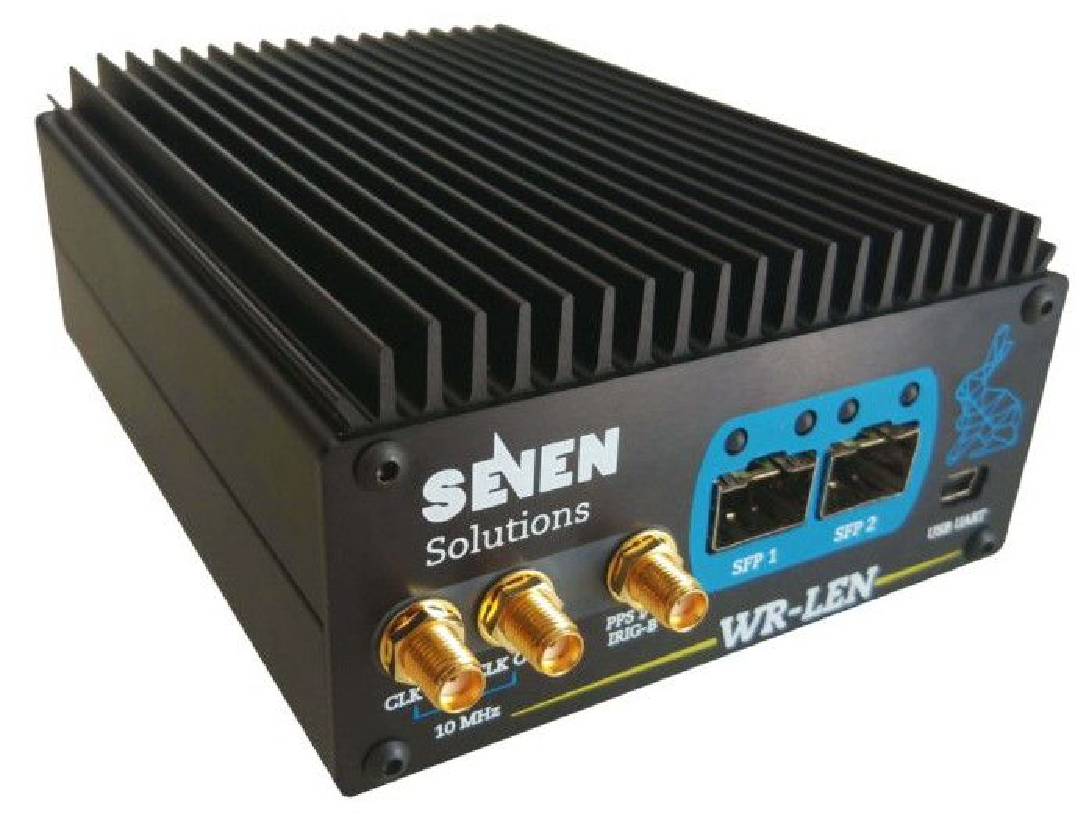
\includegraphics[height=6cm]{diagrams/5-daq/wr_len.pdf}%
    }
    \caption[Pictures of the White Rabbit timing hardware used within \chipsfive]
    {Pictures of the White Rabbit timing hardware used within \chipsfive. The compact White rabbit
        switch  specially designed for \chips is shown in (a), while the White Rabbit Lite
        Embedded Node (WR-LEN) from Seven Solutions is shown in (b).}
    \label{fig:wr_electronics}
\end{figure}

All WR components are connected using \unit{1}{\text{Gb}} bi-directional optical fibre
connections, using the \unit{1310}{\text{nm}} and \unit{1550}{\text{nm}} wavelengths via Small
Form-Factor Pluggable Transceivers (SFPs). Fig.~\ref{fig:sync} shows the subsequent WR
synchronised pulse per second clock rising edges for two \chipsfive WR switches separated by
\unit{500}{\text{m}} of fibre. With the vertical ticks representing single nanoseconds,
sub-nanosecond time synchronisation accuracy between the switches is observed.

\begin{figure} % WHITE-RABBIT SYNC DIAGRAM %
    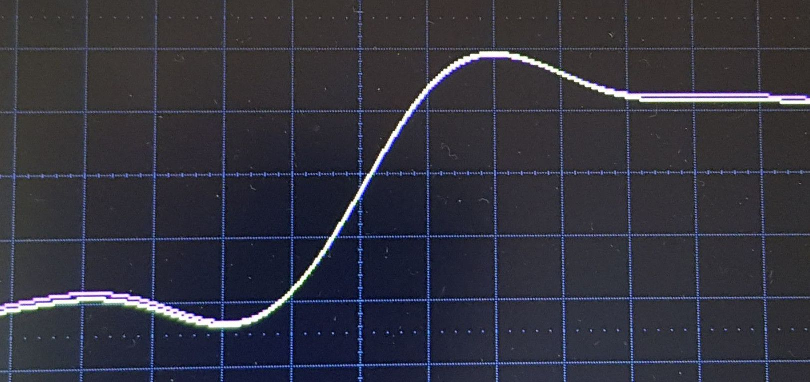
\includegraphics[width=0.7\textwidth]{diagrams/5-daq/sync.pdf}
    \caption[Picture of White Rabbit timing synchronisation seen within \chipsfive]
    {Picture of an oscilloscope display measuring the pulse per second output signal from two WR
        switches shown in pink and yellow at either end of a \unit{500}{\text{m}} long optical
        fibre. The vertical ticks are in nanoseconds showing the sub-nanosecond synchronisation
        possible with the WR timing network.}
    \label{fig:sync}
\end{figure}

\section{Hardware} %%%%%%%%%%%%%%%%%%%%%%%%%%%%%%%%%%%%%%%%%%%%%%%%%%%%%%%%%%%%%%%%%%%%%%%%%%%%%%%
\label{sec:daq_hard} %%%%%%%%%%%%%%%%%%%%%%%%%%%%%%%%%%%%%%%%%%%%%%%%%%%%%%%%%%%%%%%%%%%%%%%%%%%%%

The hardware of the \chipsfive DAQ system is split into two distinct implementations at its lower
levels (closest to the PMTs), corresponding to the Nikhef and Madison \textsc{Pom} types. \chips
R\&D efforts have principally developed the novel Madison implementation with the view to use this
hardware within detector modules exclusively. However, as a safe stepping stone, while development
and testing are still ongoing, \chipsfive mainly contains proven Nikhef hardware developed for the
KM3NeT experiment~\cite{adrian2016}.

The complete DAQ and power distribution system for \chipsfive is diagrammatically shown in
Fig.~\ref{fig:daq}. The following subsections describe each component, starting from the lowest
level and working upwards. The Nikhef and Madison descriptions are separated for clarity as well
as the high-level combined hardware systems, part of which is not physically located within the
detector but onshore in an electronics hut (separate from the water filtration hut).

\begin{figure} % DAQ DIAGRAM %
    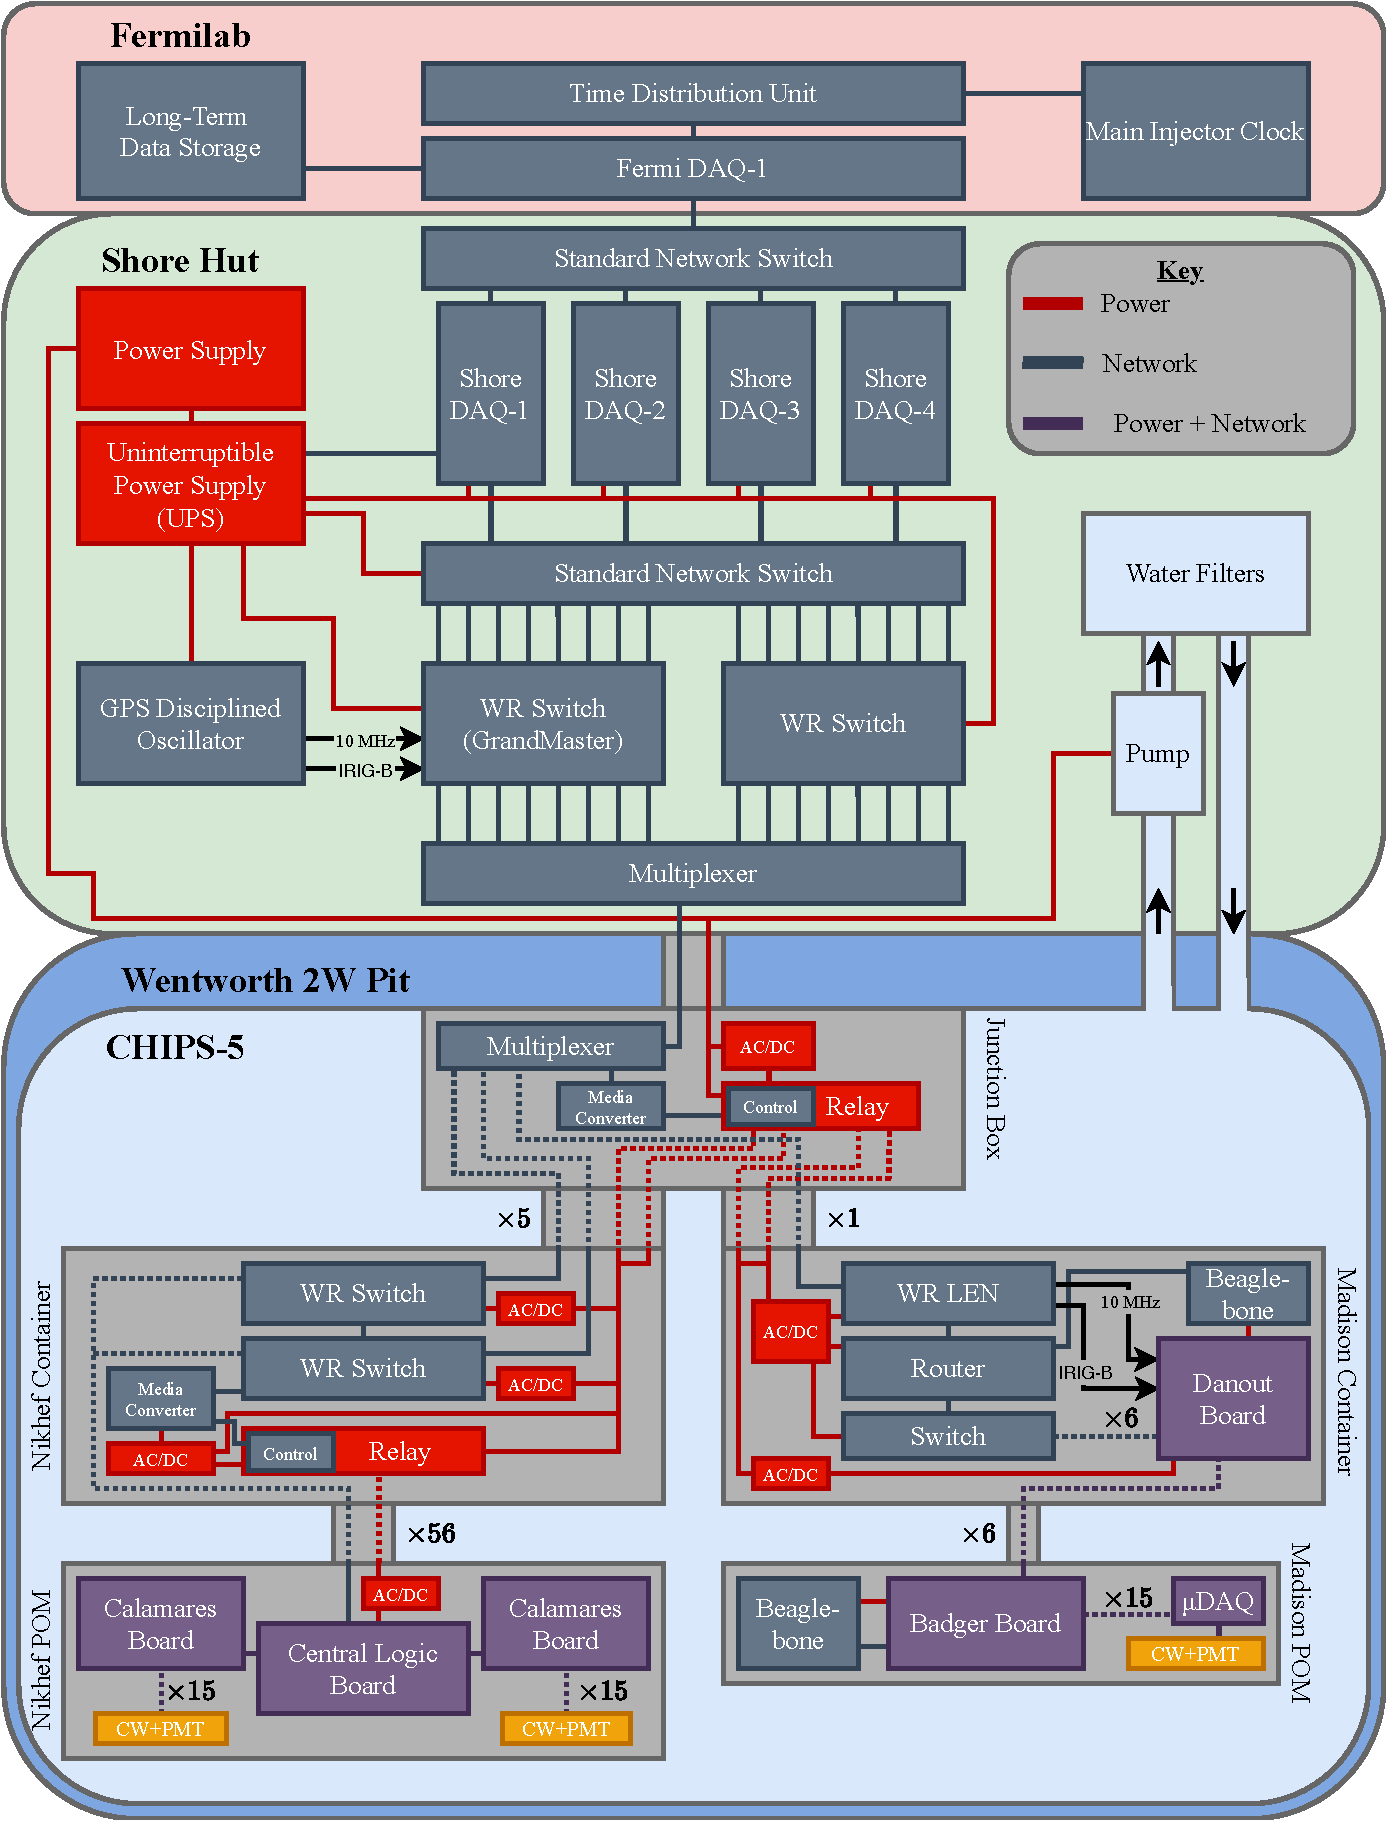
\includegraphics[width=\textwidth]{diagrams/5-daq/daq.pdf}
    \caption[Diagram of the complete \chipsfive data acquisition and power distribution system]
    {Diagram of the complete \chipsfive DAQ and power distribution system.}
    \label{fig:daq}
\end{figure}

Common to both low-level hardware implementations is the use of the Time over Threshold (ToT)
method for PMT signal digitisation. Each analogue PMT pulse is fed to a ToT discriminator coupled
with a Time to Digital Converter (TDC) to generate each digitised recorded hit, as shown in
Fig.~\ref{fig:tot}. Compared to the more common Analogue to Digital Converter (ADC) readout, ToT
values are less accurate and do not scale linearly with deposited charge. However, the ToT
methodology is used within \chips as the electronics is simpler and notably cheaper.

\begin{figure} % TOT DIAGRAM DIAGRAM %
    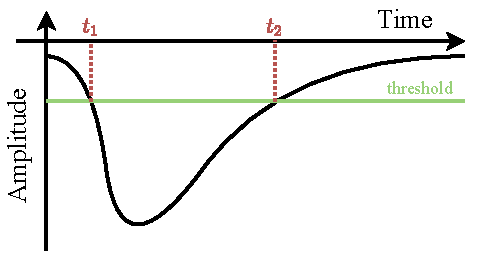
\includegraphics[width=0.6\textwidth]{diagrams/5-daq/tot.pdf}
    \caption[Illustrative diagram showing how Time over Threshold is measured]
    {Illustrative diagram showing how a ToT value is measured. As soon as the rising edge of a PMT
        charge pulse rises above a given threshold (goes below in the negative charge case) a time
        is recorded $t_{1}$, when the falling edge later falls below the threshold a second time
        $t_{2}$ is recorded. The difference in time between $t_{1}$ and $t_{2}$ is output by the
        electronics as a digitised ToT value.}
    \label{fig:tot}
\end{figure}

\subsection{Nikhef hardware} %%%%%%%%%%%%%%%%%%%%%%%%%%%%%%%%%%%%%%%%%%%%%%%%%%%%%%%%%%%%%%%%%%%%%
\label{sec:daq_hard_Nikhed} %%%%%%%%%%%%%%%%%%%%%%%%%%%%%%%%%%%%%%%%%%%%%%%%%%%%%%%%%%%%%%%%%%%%%%

All Nikhef HZC PMTs are attached directly to a simple readout board containing a high-voltage
generating Cockcroft-Walton circuit. Up to 30 such PMTs are connected to two \emph{Calamares}
boards within the electronics box of each Nikhef \textsc{Pom} via standard category 5 cables with
RJ45 connectors, as shown in Fig.~\ref{fig:nikhef_plane}. Both Calamares boards are directly
attached to a \emph{Central Logic Board} (CLB)~\cite{biagi2015, eijk2015}. The CLB contains ToT
discriminators and TDCs to digitise the recorded signals as well as electronics to synchronise to
the WR network clock for timestamping. Each Nikhef \textsc{Pom} electronics box also contains an
AC to DC power converter (AC/DC) whose output is fed into the CLB for power distribution.

\begin{figure} % NIKHEF PLANE DIAGRAM %
    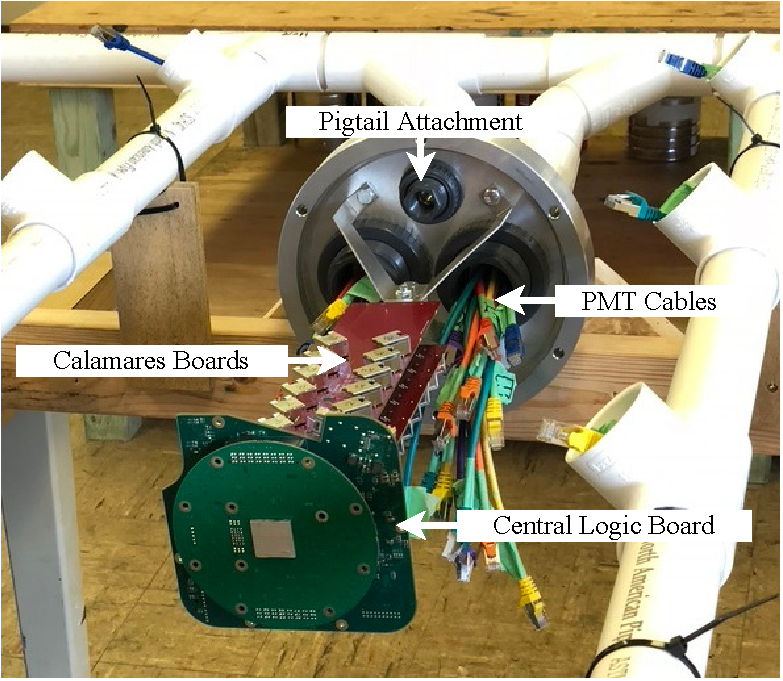
\includegraphics[width=0.8\textwidth]{diagrams/5-daq/nikhef_plane.pdf}
    \caption[Labelled picture of the Nikhef \textsc{Pom} electronics box]
    {Labelled picture of the Nikhef \textsc{Pom} electronics box without its aluminium casing.
        Both ends of the category 5 PMT cables can be seen, either at the PMT mounting points or
        entering the electronics box and not yet plugged into Calamares boards.}
    \label{fig:nikhef_plane}
\end{figure}

Every Nikhef \textsc{Pom} is connected via a single optical fibre and a single power connection to
a \emph{Nikhef-container}, the contents of which are labelled in the bottom half of
Fig.~\ref{fig:full_setup}. Two WR switches are used within each container to provide sufficient
\textsc{Pom} networking ports. Both switches are powered by independent AC to DC converters and
connected via a single optical fibre each to the higher level DAQ systems. An additional
connection between each switch ensures that if one higher-level connection fails the other can
still be used.

Each Nikhef-container also contains a relay board to control the power supply to individual
\textsc{Pom}s. The relay board control electronics are powered via an AC to DC converter and
connected to one of the switches via a media converter for networking. The media converter is
required to convert the optical fibre WR switch connection to a standard RJ45 copper cable
connection. A total of five Nikhef-containers are present within \chipsfive.

\begin{figure} % FULL SETUP DIAGRAM %
    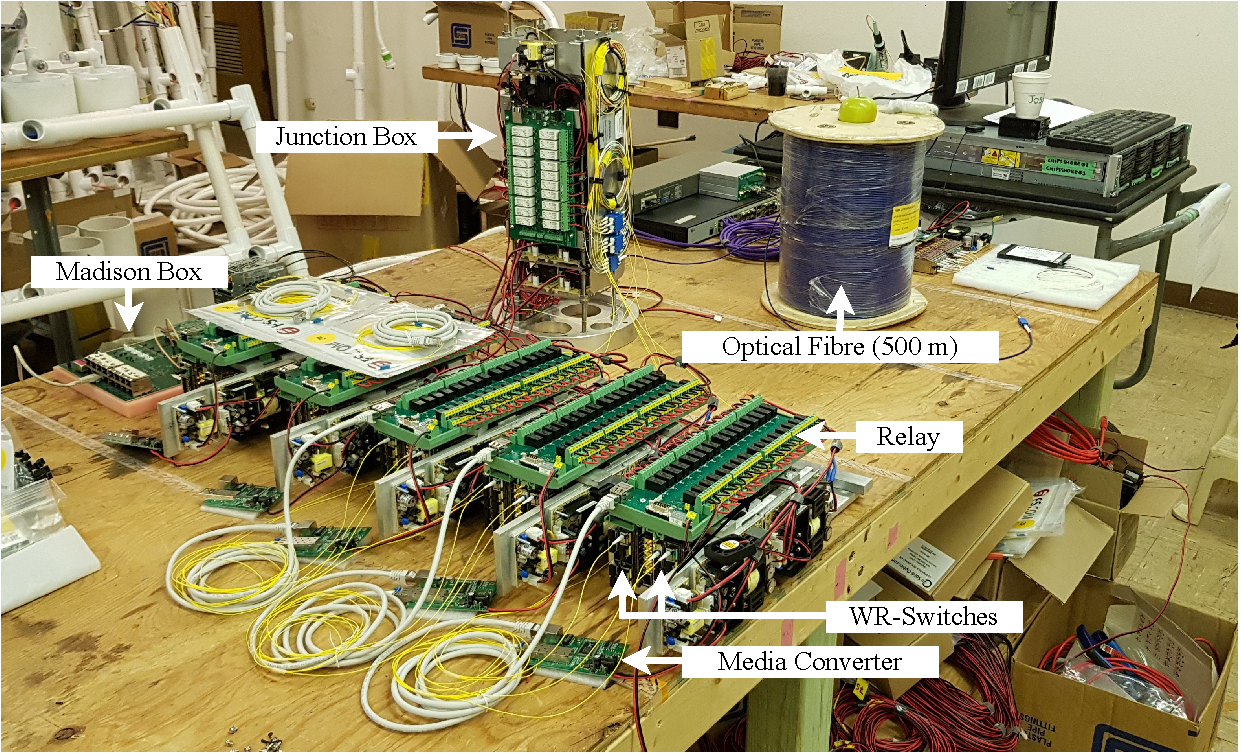
\includegraphics[width=\textwidth]{diagrams/5-daq/full_setup.pdf}
    \caption[Picture of the non \textsc{Pom} components of the \chipsfive DAQ system]
    {Picture of the non \textsc{Pom} components of the \chipsfive DAQ system arranged on a table
        at the PolyMet mining administration building.}
    \label{fig:full_setup}
\end{figure}

\subsection{Madison hardware} %%%%%%%%%%%%%%%%%%%%%%%%%%%%%%%%%%%%%%%%%%%%%%%%%%%%%%%%%%%%%%%%%%%%
\label{sec:daq_hard_madison} %%%%%%%%%%%%%%%%%%%%%%%%%%%%%%%%%%%%%%%%%%%%%%%%%%%%%%%%%%%%%%%%%%%%%

Every Madison Hamamatsu PMT is directly attached to a high-voltage generating Cockcroft-Walton
board followed by a signal processing $\micro$DAQ, as shown in
Fig.~\ref{fig:madison_pmt_assembly}. The $\micro$DAQ is a small microcontroller developed for both
IceCube and \chips at WIPAC in Madison. Capable of timestamping and digitising signals directly at
the PMT level, the $\micro$DAQ also sets the PMT operating voltage by controlling the driving
frequency of the Cockcroft-Walton board~\cite{eijk2018}.

Up to 16 $\micro$DAQs receive power, networking, and WR synchronised IRIG-B and
\unit{10}{\text{MHz}} timing signals from a \emph{badger-board}, as shown in
Fig.~\ref{fig:madison_plane}. Standard category 5 cables with RJ45 connectors are used for these
connections. The badger-board is located within the electronics box of each Madison \textsc{Pom}
and acts as a simple fanout and power control board. For logic, each badger-board has an attached
mezzanine Beaglebone~\cite{beagle2020}. This single-board Linux machine (very similar to a
Raspberry Pi) controls the power supply to, and receives hits from, the attached $\micro$DAQs.

\begin{figure} % MADISON PLANE DIAGRAM %
    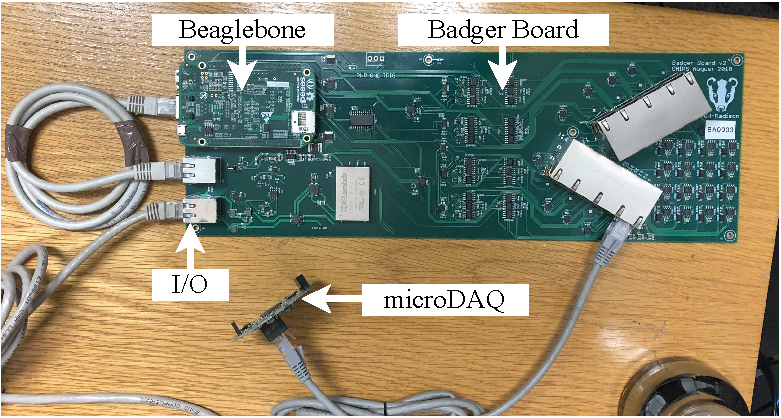
\includegraphics[width=0.8\textwidth]{diagrams/5-daq/madison_plane.pdf}
    \caption[Labelled picture of the components of the Madison \textsc{Pom} electronics box]
    {Labelled picture of the components of the Madison \textsc{Pom} electronics box.}
    \label{fig:madison_plane}
\end{figure}

Similarly, up to 16 Madison \textsc{Pom} badger-boards receive power, networking and WR
synchronised IRIG-B and \unit{10}{\text{MHz}} timing signals from a \emph{danout-board} located
within a single \emph{Madison-container}. Again, standard category 5 cables with RJ45 connectors
are used for these connections. The full contents of the Madison-container are shown in
Fig.~\ref{fig:madison_box}. Similar to the badger-board, the danout-board acts as a simple fanout
and power control board with an attached mezzanine Beaglebone. However, in this case, the attached
Beaglebone acts only to control the power provided by the danout-board.

PMT hits and other packets are instead routed through the danout-board into a networking stack.
Consisting of a WR-LEN, a router (required due to the limited WR-LEN routing table size), and a
switch (non WR), the stack provides networking to the higher-level DAQ via a single optical fibre.
The WR clock synchronised IRIG-B and \unit{10}{\text{MHz}} timing signals are output by the WR-LEN
to the danout-board for forwarding to the lower-level components. Additionally, two AC to DC
converters provide power for both the devices within the container and all lower-level components
via the danout-board.

\begin{figure} % MADISON BOX DIAGRAM %
    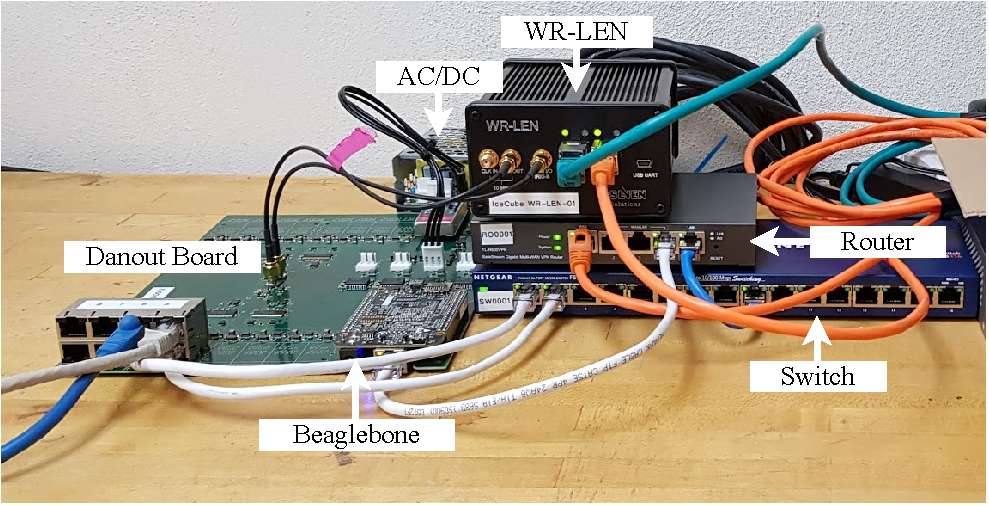
\includegraphics[width=\textwidth]{diagrams/5-daq/madison_box.pdf}
    \caption[Labelled picture of the Madison-container components]
    {Labelled picture of the Madison-container components. The blue and grey cables exiting the
        left hand side of the image go to individual Madison \textsc{Pom}s connecting to the I/O
        port shown in fig.~\ref{fig:madison_plane}. An optical fibre connection into the left SFP
        port of the WR-LEN is used in reality rather than the copper connection shown here.}
    \label{fig:madison_box}
\end{figure}

Compared to the Nikhef hardware the Madison.
\begin{itemize}
    \item By leveraging commercially available Beaglebones ($\sim£50$ each) for onboard logic and
    using vastly \textbf{cheaper} WR-LENs compared to WR switches, the Madison DAQ hardware
    implementation is drastically cheaper compared to the Nikhef (KM3NeT) approach for a minimal
    reduction in performance.
    \item By having a fully fledged Linux machine on each POM and easily reprogrammable
    $\micro$DAQ microcontrollers the DAQ software can be easily \textbf{configurable} and upgraded
    once deployed. Having so much cheap general purpose processing power close to the PMTs allows
    for most of the computation to happen at that level, additional logic can be added. Don't even
    know what we could implement yet using it. Advanced processing at lower level. 
\end{itemize}

\subsection{Combined systems} %%%%%%%%%%%%%%%%%%%%%%%%%%%%%%%%%%%%%%%%%%%%%%%%%%%%%%%%%%%%%%%%%%%%
\label{sec:daq_hard_combined} %%%%%%%%%%%%%%%%%%%%%%%%%%%%%%%%%%%%%%%%%%%%%%%%%%%%%%%%%%%%%%%%%%%%

Each Nikhef-container and Madison-container is connected to a single \emph{junction-box}, labelled
in Fig.~\ref{fig:full_setup}. This central container acts as the interface between the detector
electronics and the umbilical carrying data and power between the shore and the detector. All
connections to the junction-box (as well as those between \textsc{Pom}s and Nikhef and Madison
containers) are made within watertight, flexible PVC tubing called \emph{manifolds}. These tubes
span all corners of the \chipsfive detector, as shown in Fig.~\ref{fig:manifold}.

\begin{figure} % MANIFOLD DIAGRAM %
    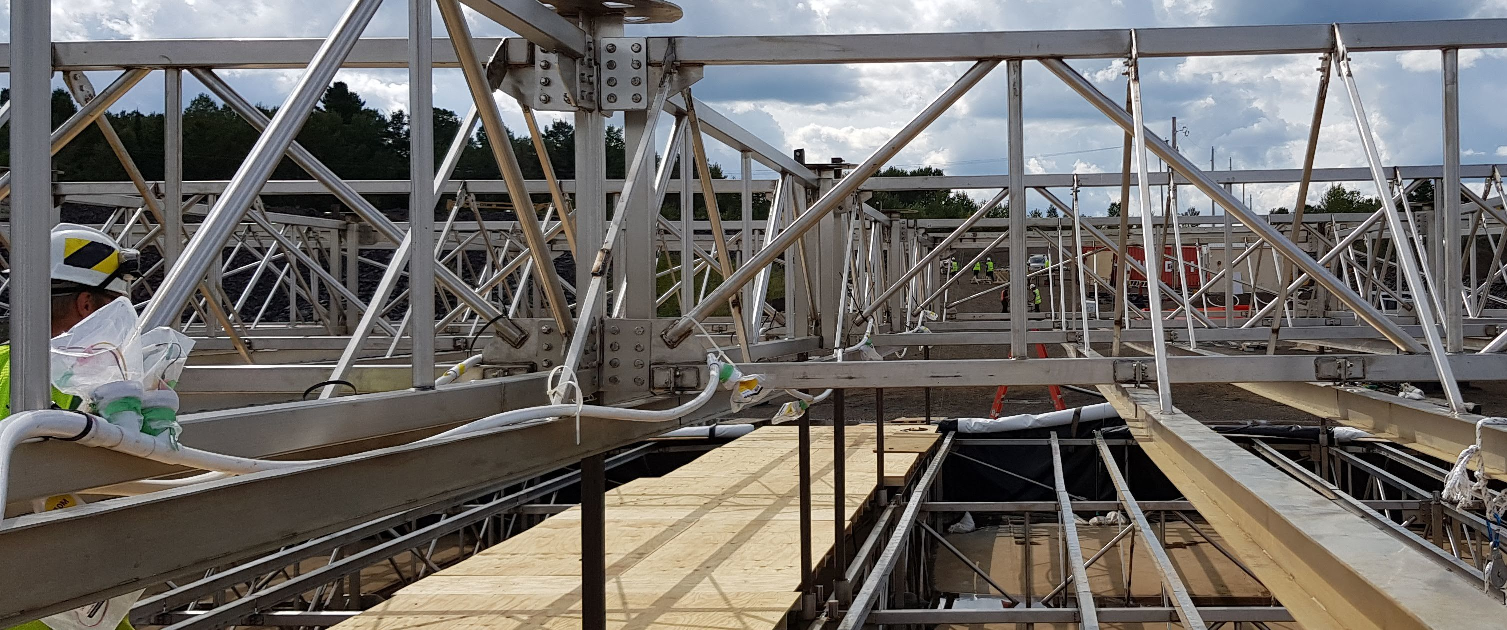
\includegraphics[width=\textwidth]{diagrams/5-daq/manifold.pdf}
    \caption[Picture of a manifold connection within the \chipsfive detector]
    {Picture of a Nikhef \textsc{Pom} to Nikhef-container manifold (in white) attached to the
        top-cap of the \chipsfive detector. In the left of the image, two unattached Nikhef
        \textsc{Pom} pigtail connections are seen, both covered in green tape and a plastic bag.}
    \label{fig:manifold}
\end{figure}

For networking the junction-box contains a Coarse Wavelength Division Multiplexing (CWDM)
multiplexer/demultiplexer (MUX/DEMUX). This device supports 32 wavelengths for a total of 16
bi-directional \unit{1}{\text{Gb}} connections over the single \unit{500}{\text{m}} long umbilical
optical fibre. Each WR-LEN or WR switch within the detector uses one of these channels exclusively
with the corresponding wavelength SFP.

The two umbilical power connections are distributed via two thick copper plates to all the relay
channels within the junction-box. Two relay boards are used to provide a sufficient number of
output channels, with their control electronics powered by separate AC to DC converters and each
connected to one of the multiplexer/demultiplexer networking channels via a media converter
(optical fibre to RJ45). Each relay channel also has a built-in \emph{trip gate} to immediately
power-off the channel if a current surge is detected. This protection is particularly crucial for
\chipsfive as water leaks are possible.

The contents of the DAQ electronics \emph{Shore Hut} are shown in Fig.~\ref{fig:hut_daq}. The
single umbilical optical fibre connection passes through a multiplexer/demultiplexer before each
of the wavelength-specific channels are passed into one of two WR switches. Multiple Virtual Local
Area Networks (VLANs) are configured on each switch such that for each wavelength channel only a
single paired port on the other physical side of the switch carries that channels data to and from
the standard networking switch (these connections are not present within Fig.~\ref{fig:hut_daq}).
Of the two WR switches, one is configured to be the GrandMaster with connections to a GPS
disciplined oscillator with an attached antenna. A single connection is also made between the WR
switches for clock synchronisation.

\begin{figure} % WHITE-RABBIT GM SETUP DIAGRAM %
    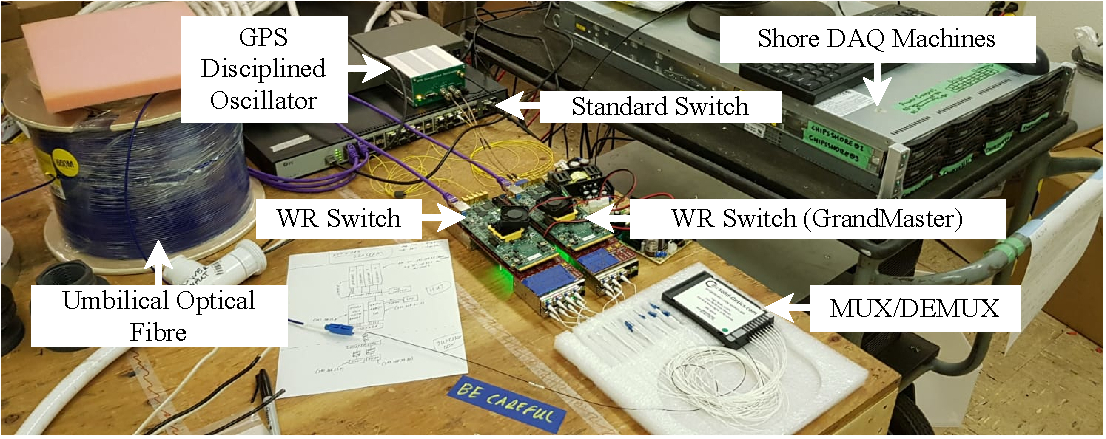
\includegraphics[width=\textwidth]{diagrams/5-daq/hut_daq.pdf}
    \caption[Picture of the onshore components of the \chipsfive DAQ system]
    {Picture of the onshore components of the \chipsfive DAQ system arranged on a table at the
        PolyMet mining administration building.}
    \label{fig:hut_daq}
\end{figure}

The standard network switch provides \unit{10}{\text{Gb}} connections to each of the Shore DAQ
computing machines whose specific roles are detailed in Section.~\ref{sec:daq_soft}. Each machine
is also connected to a second switch providing connections to the external internet and DAQ
components located at Fermilab. At Fermilab, a principle DAQ machine (Fermi DAQ-1) performs two
main roles. Firstly, it forwards \numi beam spill timing information from a Time Distribution Unit
attached to the Main Injector clock to \chipsfive. Secondly, it receives recorded detector data
from the \chipsfive located DAQ system and places it into long-term storage.

An uninterruptible power supply provides power to all devices within the Shore Hut, supplying
power for up to \unit{15}{\text{minutes}} after a power cut (sadly quite a common occurrence). The
two detector umbilical power connections do not use the uninterruptible supply and instead draw
power directly from the master supply, as does the water filtration pump.

\section{Software} %%%%%%%%%%%%%%%%%%%%%%%%%%%%%%%%%%%%%%%%%%%%%%%%%%%%%%%%%%%%%%%%%%%%%%%%%%%%%%%
\label{sec:daq_soft} %%%%%%%%%%%%%%%%%%%%%%%%%%%%%%%%%%%%%%%%%%%%%%%%%%%%%%%%%%%%%%%%%%%%%%%%%%%%%

The software of the \chipsfive DAQ system provides three main functionalities: control of the
detector instrumentation, the handling of recorded PMT hits, and the monitoring of hardware and
data quality. Each of these functions is discussed within a specific subsection below. Only the
high-level software components are detailed with the low-level CLB, Beaglebone, and $\micro$DAQ
software implementations omitted for brevity. An in-depth discussion of the CLB software can be
found in Ref.~\cite{aiello2019} while the Beaglebone and $\micro$DAQ software implementation can
be found at Ref.~\cite{microdaq2020}.

\begin{figure} % SOFTWARE DIAGRAM %
    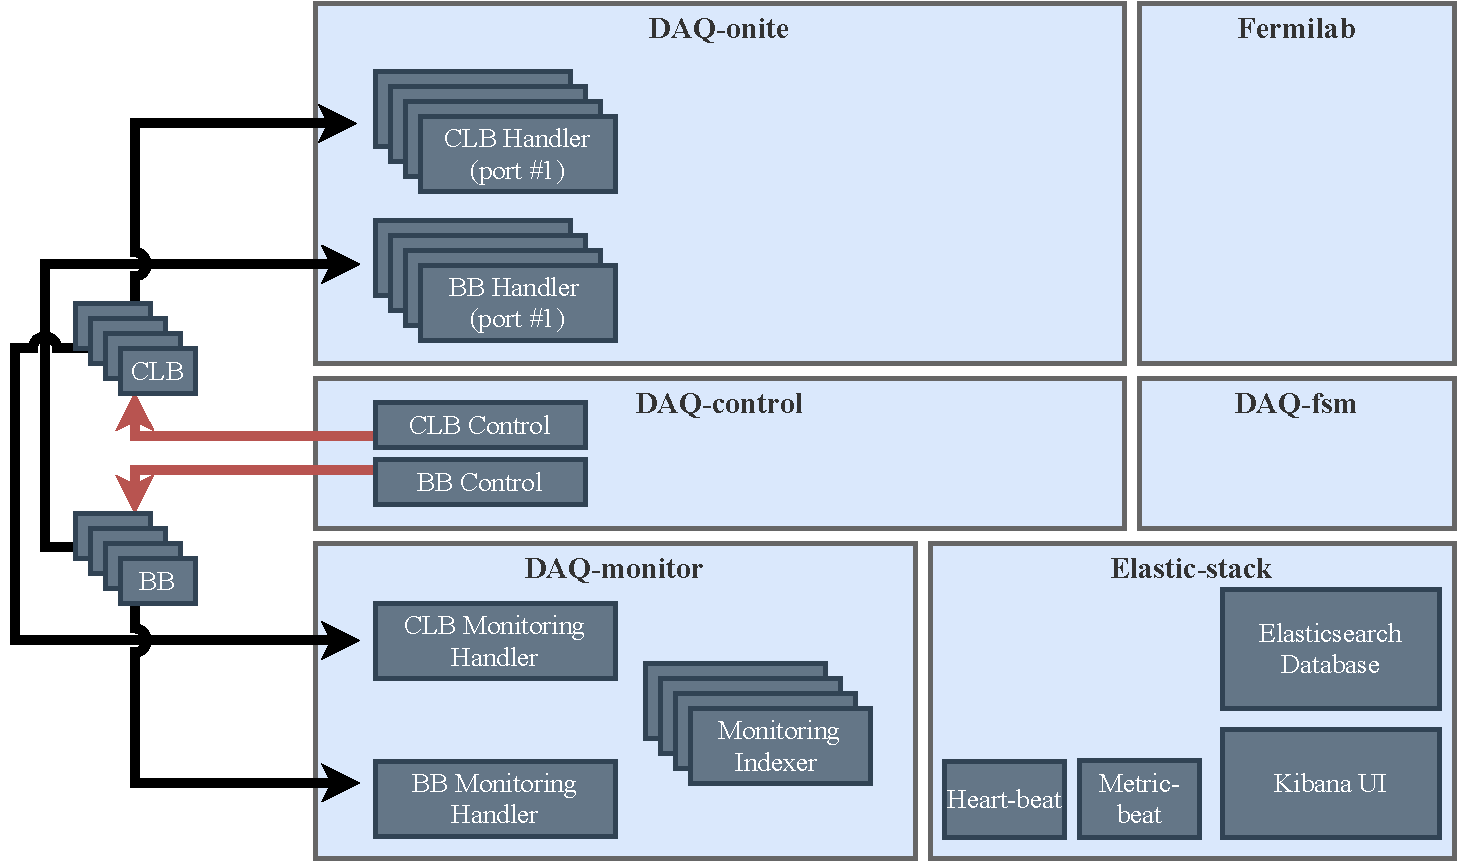
\includegraphics[width=\textwidth]{diagrams/5-daq/daq_software.pdf}
    \caption[Diagram of the \chipsfive software system in terms of the flow of data between
    components] {Diagram of the \chipsfive software system in terms of the flow of data between
    high-level components.}
    \label{fig:daq_software}
\end{figure}

The software itself is mainly written in C++ and can be found in the repository at
Ref.~\cite{chipsdaq2020}. The complete system is comprised of multiple processes, each of which is
illustratively shown within Fig.~\ref{fig:daq_software}, expressed in terms of the flow of data
between distinct software components. All DAQ processes make extensive use of multithreading and
asynchronous communication, principally implemented using the low-level Boost Asio (asynchronous
input/output) library~\cite{boost2020}. 

All central processing takes place on one of three machines: Shore DAQ-1 for hit handling, Shore
DAQ-2 control and monitoring, and Fermi DAQ-1 for \numi spill forwarding and storage. As the
processing of PMT hits is the principle software task, handled takes place exclusively on Shore
DAQ-1 without other processes to ensure maximum available processing power. Both Shore DAQ
machines have a backup machine (Shore DAQ-3 and Shore DAQ-4) to take over their functions in case
of a fault.

\subsection{Detector control} %%%%%%%%%%%%%%%%%%%%%%%%%%%%%%%%%%%%%%%%%%%%%%%%%%%%%%%%%%%%%%%%%%%%
\label{sec:daq_soft_control} %%%%%%%%%%%%%%%%%%%%%%%%%%%%%%%%%%%%%%%%%%%%%%%%%%%%%%%%%%%%%%%%%%%%%

All DAQ processes are controlled by a singular Finite State Machine (FSM) process. The FSM can be
in exactly one 

\begin{figure} % SOFTWARE DIAGRAM %
    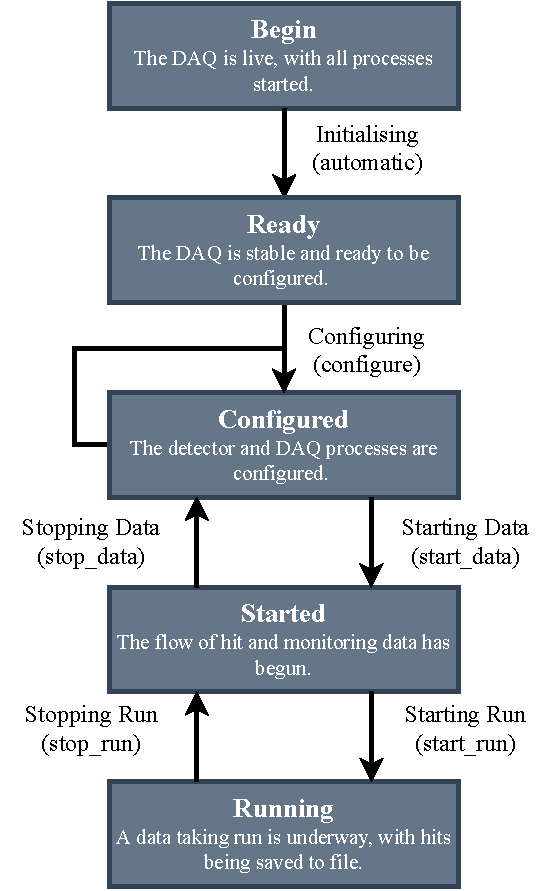
\includegraphics[width=0.6\textwidth]{diagrams/5-daq/fsm.pdf}
    \caption[fsm]
    {fsm}
    \label{fig:fsm}
\end{figure}

- inspired by the KM3NeT Java implementation
A singular Finite State Machine (FSM) process on DAQ
- Finite State Machine (FSM)
- DHCP server controls all the static ip addresses!
- Sometimes referred to as slow-control
- typically this is separated physically into a separate network, that is the best way to do the
DAQ for multiple reasons, but this would make the \chips DAQ system dramatically more complicated,
as running another cable requires so much more effort than normal, so they are combined into one.
- The detector is configured using a single human readable configuration file that defines all the
\textsc{Pom} types, MAC addresses, IP addresses, types, relay channels, which channels should be active and
their associate high voltage setting, threshold and electronic ID.
- Taking inspiration from the KM3NeT DAQ Java software
- Currently no run control system is in place to automatically control the detector according to a
scheduled run plan. Detector control is done via a simple command line interface (CLI) that
communicates with the FSM. Starting data taking, starting runs of a given type, stopping,
configuring with a given configuration file etc...

\subsection{Hit acquisition} %%%%%%%%%%%%%%%%%%%%%%%%%%%%%%%%%%%%%%%%%%%%%%%%%%%%%%%%%%%%%%%%%%%%%
\label{sec:daq_soft_hits} %%%%%%%%%%%%%%%%%%%%%%%%%%%%%%%%%%%%%%%%%%%%%%%%%%%%%%%%%%%%%%%%%%%%%%%%

As in done within KM3NeT, an `all-data-to-shore' approach is taken, where all PMT hit data is sent
via the WR network to the machines on shore. No triggering takes place within the detector. This
is done by collecting all PMT hits on each low level device (CLB or Beaglebone) within time
windows, \unit{10}{\mathrm{ms}} in length. At the end of each window, data is packaged along with
a header into User Datagram Protocol (UDP) packets and sent to shore. 

UDPavoids the overhead of error checking and correction processes, as this should be low it is not
required as allows for a higher bandwidth data stream to shore.

- How the beam spill stuffy works and how it is used to trigger hit acquisition
- Talk about the data rates for hits at full steam
- Jumbo frames etc
- Data is sent in UDP packets (not TCP so some will go missing)
- Typical ethernet frame has a maximum transmission unit (MTU) size of 1500 bytes, we use Jumbo
frames that allow for an MTU of 9000 bytes, this means we have a lot less small frames with only a
limited number of recorded hits, which proved to be taxing to the switches and lead to an increase
in the number of dropped frames.
- 1Gb links between WR switches, 10Gb link between FS switch and main DAQ machine. Provides
sufficient bandwidth, DO A SMALL CALCULATION!

\subsection{Monitoring} %%%%%%%%%%%%%%%%%%%%%%%%%%%%%%%%%%%%%%%%%%%%%%%%%%%%%%%%%%%%%%%%%%%%%%%%%%
\label{sec:daq_soft_monitor} %%%%%%%%%%%%%%%%%%%%%%%%%%%%%%%%%%%%%%%%%%%%%%%%%%%%%%%%%%%%%%%%%%%%%

- Talk about the data rates for monitoring at full steam
- Which machines run this, which is backup?

- Elasticsearch ref in~\cite{elastic2020}
- An open source RESTful, JSON-based, search engine and noSQL database.
- Data is stored in \emph{indices} in individual \emph{documents}
- Get to leverage an enormous amount of online support and the community
- daqlog: Uses for DAQ application logging with a severity
- daqstate: Used to report the current state of various DAQ applications
- monpom: Used for reporting general \textsc{Pom} monitoring information, such as temp, humidity, status
- monchannel: Used for reporting individual channel monitoring, such as rate, veto
- A series of altering rules are also set up constantly monitoring the status of the monitoring
data contained within the elasticsearch database to alert via slack or email individuals if something goes wrong.
- We index asynchronously to not block data taking, all data is backed up easily.
- Use the Kibana user interface which is accessible through a browser, means that no special
equipment, or GUIs are used, anyone on any machine has access to the full monitoring stack from
their browser. A series of dashboards ar set up to monitor everything within the detector.
- A series of indices are set up to store data which is sent via standard REST messages to the
database, the special indexing allows for quick `searching' over any time period etc... for
monitoring.
- Also means that anyone can quickly/easily look at any part of the data and make plots etc...
without needing to write an additional part of a monitoring program.
- Means the full detector and data quality monitoring is accessible to anyone with access anywhere
in the world via their normal browser.

\begin{figure} % MONITORING DIAGRAM %
    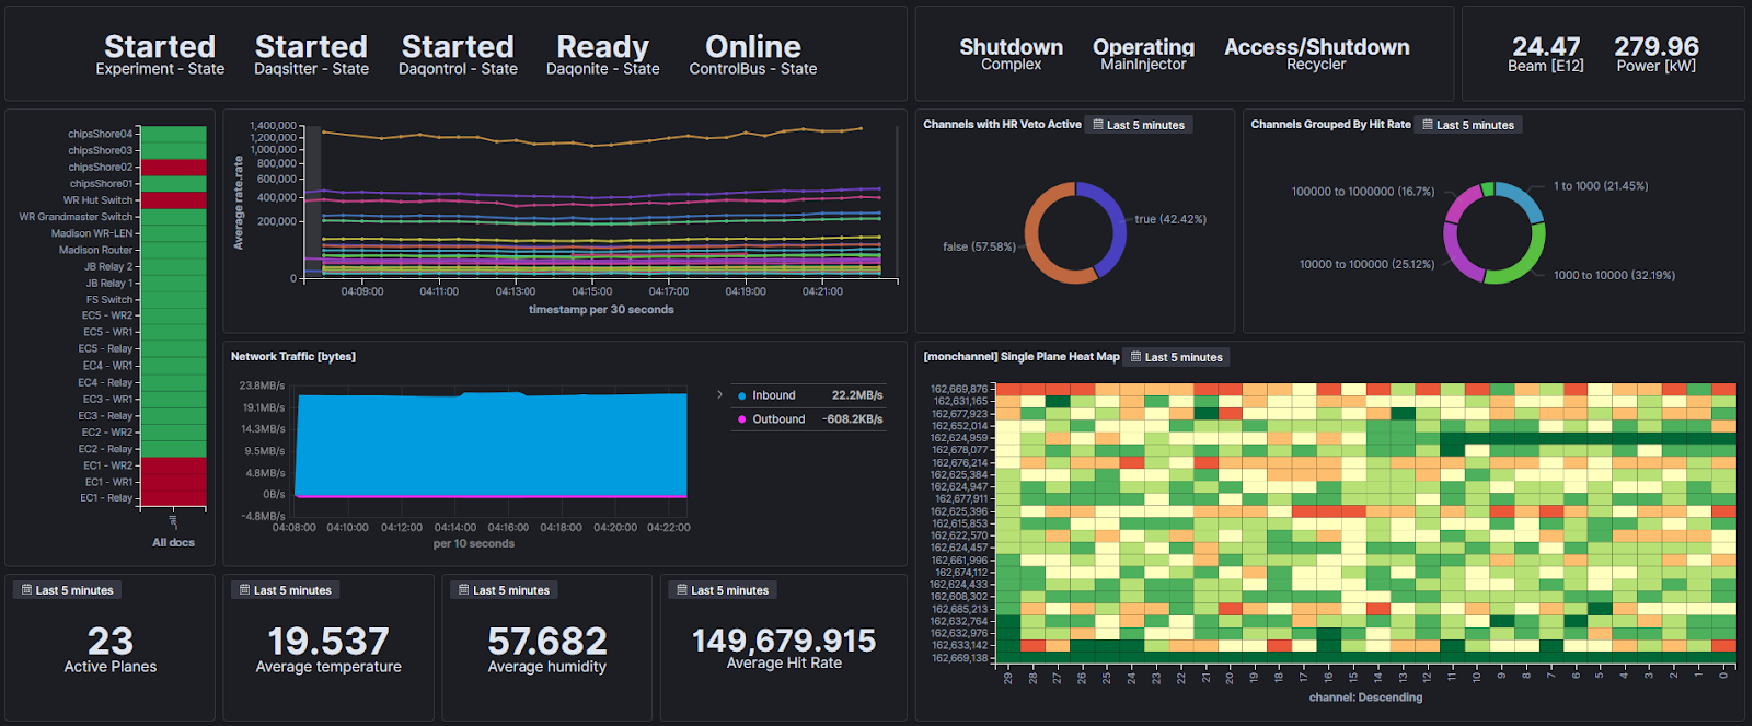
\includegraphics[width=\textwidth]{diagrams/5-daq/monitoring.pdf}
    \caption[monitoring short]
    {monitoring long}
    \label{fig:monitoring}
\end{figure}
    \chapter{Convolutional neural networks for CHIPS} %%%%%%%%%%%%%%%%%%%%%%%%%%%%%%%%%%%%%%%%%%%%%%%%
\label{chap:cvn} %%%%%%%%%%%%%%%%%%%%%%%%%%%%%%%%%%%%%%%%%%%%%%%%%%%%%%%%%%%%%%%%%%%%%%%%%%%%%%%%%

For the majority of HEP experiments, event analysis has two primary aims. The separation of signal
events from background events and the estimation of particle energies. The same is true for
\chips, with the primary aims being the selection of CC $\nu_{e}$ signal events from a sizeable
background and the estimation of the associated neutrino energy.

For this purpose, the \chips project has so far relied on a complex human implemented
reconstruction algorithm and a simple classification \emph{neural network} driven by
hand-engineered features. Both of which are prone to human error and restricted in scope to what
has been implemented in software.

The work outlined in this chapter presents a replacement event analysis methodology for \chips.
Three \emph{Convolutional Neural Networks} (CNNs) a type of \emph{deep learning} neural network
have been implemented to achieve the goals outlined above. One for cosmic muon rejection, one for
beam classification, and one for neutrino energy estimation.

After covering previous deep learning implementations for neutrino experiments, a brief
description of the current techniques to be replaced is made. The theoretical background to CNNs
is then outlined before the baseline implementation for \chips is described. Finally, the three
separate networks are discussed, and their combined performance presented.

\section{Previous applications of deep learning for neutrino experiments} %%%%%%%%%%%%%%%%%%%%%%%%
\label{sec:cvn_previous} %%%%%%%%%%%%%%%%%%%%%%%%%%%%%%%%%%%%%%%%%%%%%%%%%%%%%%%%%%%%%%%%%%%%%%%%%

Over the last few years, neutrino experiments have started to adopt deep learning techniques for a
range of tasks. This trend has followed the general explosion of interest in the field amongst the
global research community, especially within computer vision, as can be seen in
Fig.~\ref{fig:papers}.

\begin{figure} % NUMBER OF PAPERS DIAGRAM DIAGRAM %
    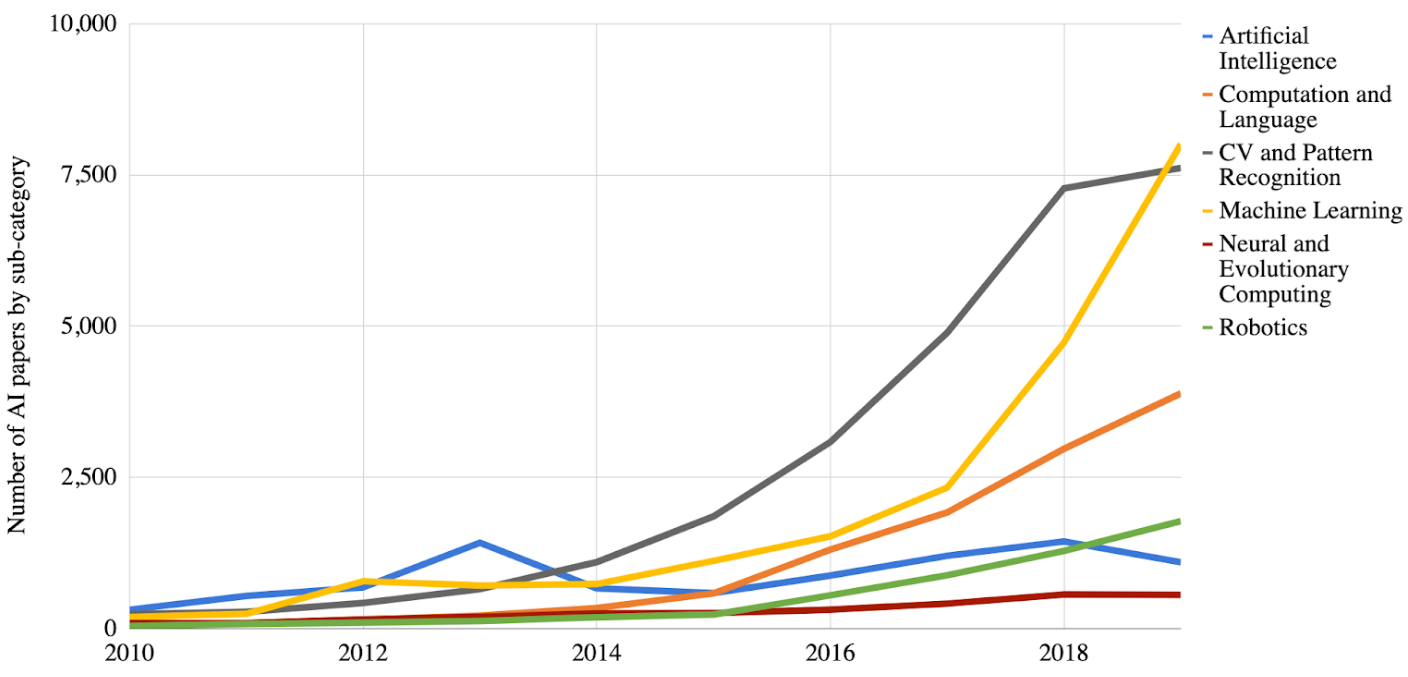
\includegraphics[width=0.8\textwidth]{diagrams/6-cvn/papers.png}
    \caption[papers short]
    {The number of artificial intelligence papers submitted to arXiv, broken down by sub-category.
        Note the particularly large increase in Computer Vision (CV) and pattern recognition
        papers. Figure taken from Ref.\cite{perrault2019}.}
    \label{fig:papers}
\end{figure}

In 2016 the \nova experiment applied a CNN to the task of classifying the interaction type of
events within their sampling calorimeter detector~\cite{aurisano2016}. Two views of raw detector
events were used as input to train a network based on the popular GoogLeNet
architecture~\cite{szegedy2015}, discussed in section \ref{sec:cvn_theory_conv}. An improved
iteration has since been applied to both the classification of individual energy deposit
clusters~\cite{psihas2019} and $\nu_{e}$ and $e^{-}$ energy reconstruction~\cite{baldi2019}.

CNNs have also been applied to liquid argon time-projection chambers. The MicroBooNE experiment
has shown that in addition to classification tasks, the localisation of single particles within
events is possible~\cite{acciarri2017}. Furthermore, the DUNE collaboration has designed a network
to output both the interaction class and counts of different particle types in an
event~\cite{collaboration2020, abi2020}. This approach is called \emph{multi-task} learning and is
discussed in detail within Section.~\ref{sec:cvn_baseline_multi}.

Applications to water Cherenkov detectors have also been made, by both the Daya Bay reactor
experiment~\cite{racah2016} and the KM3NeT/ORCA collaboration~\cite{aiello2020}. Additionally, a
type of network known as a \emph{variational autoencoder} has been shown to approximate the
distribution of simulated water Cherenkov data~\cite{abhishek2019}. If further studies prove
successful, this could allow for training on real data to reduce experimental uncertainties and
increase the speed of simulated data generation by many orders of magnitude.

\section{Standard event reconstruction and classification} %%%%%%%%%%%%%%%%%%%%%%%%%%%%%%%%%%%%%%%
\label{sec:cvn_old} %%%%%%%%%%%%%%%%%%%%%%%%%%%%%%%%%%%%%%%%%%%%%%%%%%%%%%%%%%%%%%%%%%%%%%%%%%%%%%

It is essential to outline the standard event reconstruction and classification methods that have
been used by the \chips project up till now. This is key for two main reasons. Firstly, to add
context for comparison with the new CNN approach, as is done in
Section~\ref{sec:cvn_final_comparison}. Secondly, to highlight the main weaknesses of these
methods, motivating the new technique and making its advantages clear.

A \emph{maximum likelihood} method based on that implemented by MiniBooNE~\cite{patterson2009} is
used for event reconstruction. Additionally, a simple neural network built using the TMVA
package~\cite{hocker2007} and using outputs from the reconstruction is used for event
classification. Both methods are very typical of the mainstream approach used by the majority of
water Cherenkov neutrino experiments. A prime example is the fiTQun algorithm developed for the
Super-Kamiokande detector, which is now used for both atmospheric~\cite{jiang2019} and
T2K~\cite{missert2017} analyses.

Due to the limited resources of the \chips collaboration, it is a certainty that both the event
reconstruction and classification do not represent an optimal implementation of these methods.
However, any possible improvements would be small relative to those introduced by the CNN
approach. Therefore, for comparisons, it is reasonable to assume they approximate the maximum
performance these approaches can provide.

\subsection{Likelihood based reconstruction} %%%%%%%%%%%%%%%%%%%%%%%%%%%%%%%%%%%%%%%%%%%%%%%%%%%%%
\label{sec:cvn_old_reco} %%%%%%%%%%%%%%%%%%%%%%%%%%%%%%%%%%%%%%%%%%%%%%%%%%%%%%%%%%%%%%%%%%%%%%%%%

The event reconstruction methodology is simple in theory: for a given set of hypothesised tracks,
the number of photoelectrons and the time at which the first of these is recorded for each PMT in
the detector is predicted. By comparing this prediction with the measured hit charges and times
the likelihood that the given track hypothesis produced the measured signals can be calculated.
The parameters that describe the hypothesised tracks are then varied until the negative logarithm
of the likelihood is minimised. Identifying the best-fit parameters for the hypothesis. A brief
description of the procedure is given below, however, for a full description see
Ref.~\cite{blake2016} and in great detail Ref.~\cite{perch2017}.

The first stage of event reconstruction is the effective \emph{seeding} of tracks that are then
used in the full likelihood fit. The seeding methods aim to provide a good starting point for the
minimisation, both to increase the efficiency of finding the optimal track parameters and also to
avoid a false local minimum from being returned.

Firstly, the PMT hits are sliced in both space and time. Gaps in the time ordering of hits are
used to separate the event into time slices. Each of these then undergoes basic filtering and
clustering to remove outlying hits and ensure only the dominant collections of hits are
considered. Each cleaned slice is then run through simple vertex finding algorithms to estimate
the interaction position and time, as well and the initial track direction.

A circular \emph{Hough transform} algorithm, traditionally used for water Cherenkov ring finding
is then applied. The voting-based transformation produces as output a space within which rings of
PMT hits exist as single peaks. The track direction values are then further refined using this
space, and a search for smaller peaks is carried out to indicate if multiple particles are likely
to be involved. This process results in a list of seeds with a corresponding score related
directly to the height of the associated peak in Hough transform space.

Each track in a fit hypothesis is made up of a vector of parameters $\vec{x}$, containing the
following:
\begin{itemize}
    \item The track vertex position ($x_{0}$, $y_{0}$, $z_{0}$) and interaction time $t_{0}$.
    \item The initial track direction ($d_{\theta}$, $d_{\phi}$).
    \item The initial kinetic energy of the particle.
    \item The particle type (muon, electron or photon).
\end{itemize}
Additionally, for a photon hypothesis (identical to an electron hypothesis in reality) the
distance between the interaction vertex and the beginning of the electromagnetic shower is
included as a parameter.

All the tracks in the hypothesis are then initialised using those found in the seeding procedure
in descending order of Hough peak height score. As the seeding algorithms do not estimate the
particle energy, a default value equal to the average particle energy observed in the Monte Carlo
simulation is assigned. Additionally, constraints can be placed on multi-track fits before the
minimisation process begins to reduce the number of free parameters.

For example, in the NC $\pi^{0}$ case, a multi-track two-photon hypothesis is used. Firstly, the
initial parameters for the two photons are assigned from the two highest-scoring seeds. Secondly,
the vertex position for both tracks is constrained to remain the same, and the directions and
energies are set to be constrained by the invariant mass of the $\pi^{0}$.

In it's simplest form the likelihood is a simple product of two terms:
\begin{equation} % LIKELIHOOD EQUATION %
    \mathcal{L}(\vec{x})=\mathcal{L}_{unhit}(\vec{x})\mathcal{L}_{hit}(\vec{x})=
    \prod_{unhit}P_{unhit}(\vec{x})\prod_{hit}P_{charge}(\vec{x})P_{time}(\vec{x}),
    \label{eq:likelihood}
\end{equation}
where the first ($unhit$) gives the likelihood that the hypothesis $\vec{x}$ will not predict a
hit on the PMTs that do not have a measured hit, and the second ($hit$) gives the likelihood that
$\vec{x}$ produces the observed photoelectrons and hit times on the hit PMTs. By considering the
negative logarithm of the likelihood instead, the computation can be simplified into a sum of
logarithms over the PMTs, such that
\begin{equation} % LIKELIHOOD SUM PMTS EQUATION %
    -\log\mathcal{L}(\vec{x})=
    -\sum_{unhit}\log(P_{unhit}(\vec{x}))
    -\sum_{hit}\log(P_{charge}(\vec{x}))
    -\sum_{hit}\log(P_{time}(\vec{x})).
    \label{eq:likelihood_sum}
\end{equation}
This also has the effect of separating the charge (number of photoelectrons) and time prediction
components which can then be dealt with separately computationally. In the actual likelihood
calculation the $P_{unhit}(\vec{x})$ and $P_{charge}(\vec{x})$ components are combined, where the
probability of an unhit PMT is treated as a PMT with observed charge equal to zero.

The Minuit2 algorithm contained within ROOT~\cite{brun1997} is used for the minimisation process.
At each iteration, the charge and hit time predictions are made, and the negative logarithm of the
likelihood is calculated. The track parameters are then varied to minimise the likelihood before
the next iteration. Through a series of stages, fixing and then freeing specific parameters, the
minimisation process converges to the best-fit parameters for the given hypothesis. This process
typically takes two minutes on a standard batch farm computing node.

The charge and hit time predictions and their associated likelihood contributions rely on many
low-level inputs to the reconstruction. These generally describe how Cherenkov light is emitted
from specific particles and then propagates through the detector medium to be detected by the
PMTs. Examples of these inputs include the following:
\begin{itemize}
    \item The number of Cherenkov photons emitted by a particle of specific type and energy.
    \item The fraction of Cherenkov light emitted at each step along a specific particles track
          length.
    \item The angular distribution of Cherenkov photon emission for each type of particle.
    \item The survival probability of photons within the detector medium as a function of
          distance.
    \item A detailed description of the PMT positions and directions within the detector.
    \item The angular efficiency of each PMT relative to the incident photon angle.
    \item The probability of a measured charge given the predicted number of photoelectrons
          (derived from a reversal of the simulation digitisation methodology).
\end{itemize}
The first three are combined into \emph{emission profiles} generated from large samples of the
Monte Carlo simulation, one representation of which is very similar to those shown in
Fig.~\ref{fig:emission_profile}. Additionally, the last listed input is equal to that shown in
Fig.~\ref{fig:digitisation}.

The list above demonstrates a fundamental problem with the likelihood-based approach. It is
heavily reliant on the accuracy of low-level inputs and their associated use in human implemented
software. If a physical process is not dealt with appropriately or overlooked, then the prediction
accuracy of charges and hit times for the PMTs is affected, impacting the performance of finding
the correct best-fit parameters.

The other fundamental flaw of the likelihood-based approach is the requirement of a predefined
track hypothesis. Real events expected within \chips are rarely simple single particle or even
two-particle events. In reality, the majority of events contain multiple final state particles of
various types and in various topologies. The predefinition of a track hypothesis makes it
impossible to implement a generalised approach to event reconstruction where all possible event
types are considered and explored.

\subsection{Event classification}%%%%%%%%%%%%%%%%%%%%%%%%%%%%%%%%%%%%%%%%%%%%%%%%%%%%%%%%%%%%%%%%%
\label{sec:cvn_old_pid} %%%%%%%%%%%%%%%%%%%%%%%%%%%%%%%%%%%%%%%%%%%%%%%%%%%%%%%%%%%%%%%%%%%%%%%%%%

As the reconstruction is based on the calculation of a likelihood (analogous to a
\emph{goodness-of-fit}), the likelihood ratio between different hypotheses can be used for event
classification tasks. It is also found that additional hand-engineered features derived from the
reconstruction outputs have power in classifying the event type.

Two simple neural networks are used, the first for CC $\nu_{e}$ - CC $\nu_{\mu}$ separation and
the second for CC $\nu_{e}$ - NC separation. Both contain a single hidden layer, with the number
of nodes equal to the number of input parameters plus five. Variables from both a single $e$ track
and single $\mu$ track hypothesis fit to every event are used for both networks, with a full list
of inputs as follows:
\begin{itemize}
    \item The $\Delta\log\mathcal{L}$ between $e$ and $\mu$ hypothesis for both time and charge
          components.
    \item The total number of hit PMTs ($N_{hits}$) and total collected charge.
    \item $\frac{\Delta\log\mathcal{L}_{charge}}{N_{hits}}$.
    \item The fraction of hits inside the central hole, within, and outside the ring for both $e$
          and $\mu$ hypotheses.
    \item The fraction of predicted charge outside the ring for both $e$ and $\mu$ hypotheses.
    \item The ratio of the total predicted charged to the total measured charge for both $e$
          and $\mu$ hypothesis.
    \item The ratio of the reconstructed energy to the total measured charge.
    \item The reconstructed track direction under the $e$ hypothesis.
    \item The fraction of hits in the downstream half of the detector.
    \item The number of seeds generated by the Hough transform seeding algorithm.
    \item The peak height score of the first and last seeds found by the Hough transform seeding
          algorithm.
\end{itemize}

A sample of CC $\nu_{e}$ and CC $\nu_{\mu}$ beam events characteristic of those expected to be
seen by \chips is used to train the first classifier, and a corresponding sample of CC $\nu_{e}$
and NC events for the second. Both output values can then be used to classify events into separate
samples for further analysis.

The main limitation of this approach is that the input features are restricted to those that have
been imagined (requiring extensive domain knowledge) and then implemented in software. The current
list is almost certainly non-exhaustive of all the possible variables and combinations of
variables that can, in theory, be used for discrimination between events. Additionally, any
mistakes in the likelihood-based reconstruction and, therefore, input variables to the neural
networks can lead to incorrect categorisation of events.

\section{The theory of neural networks} %%%%%%%%%%%%%%%%%%%%%%%%%%%%%%%%%%%%%%%%%%%%%%%%%%%%%%%%%%
\label{sec:cvn_theory} %%%%%%%%%%%%%%%%%%%%%%%%%%%%%%%%%%%%%%%%%%%%%%%%%%%%%%%%%%%%%%%%%%%%%%%%%%%

There are many machine learning techniques: linear regression, logistic regression, k-nearest
neighbours, decision trees, random forests, support vector machines, all of which learn to make
predictions about data. However, none have been as successful, especially in recent years, as the
deep neural network. As both the size of datasets and the amount of available computational power
has increased, deep neural networks have proven the most powerful technique for many tasks as they
are well suited to this paradigm.

Here we discuss the application of neural networks for \emph{supervised learning}, one of two
broad machine learning categories that is concerned with using labelled example data to train the
algorithm. The other category of \emph{unsupervised learning}, where the properties the dataset
are inferred without example data is not discussed, however, will be used
Section.~\ref{sec:cvn_explain}.

\subsection{Neural network basics} %%%%%%%%%%%%%%%%%%%%%%%%%%%%%%%%%%%%%%%%%%%%%%%%%%%%%%%%%%%%%%%
\label{sec:cvn_theory_basics} %%%%%%%%%%%%%%%%%%%%%%%%%%%%%%%%%%%%%%%%%%%%%%%%%%%%%%%%%%%%%%%%%%%%

A neural network is a type of algorithm inspired by the repeating cell structure of neurons within
our brains. The basic building block of a neural network is a \emph{neuron} which takes a vector
of $k$ inputs $\vec{x} = (x_{1}, x_{2},\dots,x_{k})$ and outputs a scalar $a(\vec{x})$. The
neurons are arranged into layers, with the input of one layer being the output from the previous
layer. The first layer is commonly referred to as the \emph{input layer}, the middle layers as
\emph{hidden layers}, and the final layer as the \emph{output layer}, as illustrated in
Fig.~\ref{fig:network}. In general, this simple neural network structure is referred to as
\emph{fully-connected} as all the neurons in each layer have connections to all the neurons in the
previous and following layers.

\begin{figure} % BASIC NETWORK DIAGRAM %
    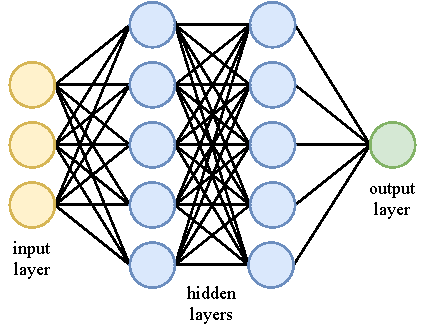
\includegraphics[width=0.6\textwidth]{diagrams/6-cvn/network.pdf}
    \caption[Illustration of a simple neural network]
    {Illustration of a simple neural network. There is a single input layer (yellow), two hidden
        layers (blue), and an output layer (green). Each node corresponds to a \emph{neuron}
        except for the input layer.}
    \label{fig:network}
\end{figure}

Input variables (traditionally hand-engineered features extracted from the raw data) are passed
into the network via the input layer. Any number of hidden layers containing any number of neurons
can then follow. The neurons contained within these layers are trained so that collectively their
$a(\vec{x})$ functions solve the problem at hand. For a \emph{regression} task, the output layer
outputs a continuous decimal value. Otherwise, for a \emph{classification} task, a probability
value between zero and one is output for each class. The forward passing of information from one
layer to the next is why neural networks can also be referred to as \emph{feed-forward graphs}.

For a neuron $i$, $a_{i}(\vec{x})$ can be decomposed into a linear operation, specific to the
neuron, followed by a non-linear operation, which is the same across all neurons. The linear
operation consists of the dot product of the input vector $\vec{x}$ with a vector of weights
$\vec{w}^{(i)} = (w_{1}^{(i)}, w_{2}^{(i)},\dots,w_{k}^{(i)})$, which weight the relative
importance of the inputs, plus a bias term $b^{(i)}$:
\begin{equation} % NETWORK BASIC EQUATION %
    z^{(i)}=\vec{w}^{(i)}\cdot\vec{x}+b^{(i)}.
    \label{eq:network}
\end{equation}
After applying the non-linear operation $\sigma_{i}$, commonly referred to as the \emph{activation
    function} the final output from the neuron can be written as
\begin{equation} % NETWORK ACTIVATION EQUATION %
    a_{i}(\vec{x})=\sigma_{i}(z^{(i)}).
    \label{eq:activation}
\end{equation}

Traditionally, a step-function (for networks called \emph{perceptrons}) was used for the
activation function. However, as is shown in Section.~\ref{sec:cvn_theory_training}, a non-zero
gradient (only valid at $x=0$ for a step-function) is required for the practical training of
neural networks. In fact, the choice of activation function can greatly affect how the network
trains and performs.

Therefore, common choices have been the \emph{hyperbolic tangent} and the \emph{sigmoid} function,
primarily because they are bounded and differentiable at all points. Recently, the \emph{ReLU} and
other similar functions have become popular, especially for CNNs. This is mainly due to them
avoiding the problem of \emph{vanishing} gradients caused by the saturation of the tanh and
sigmoid functions at large values of $x$. All of these functions are shown in
Fig.~\ref{fig:activations}.

\begin{figure} % ACTIVATIONS DIAGRAM %
    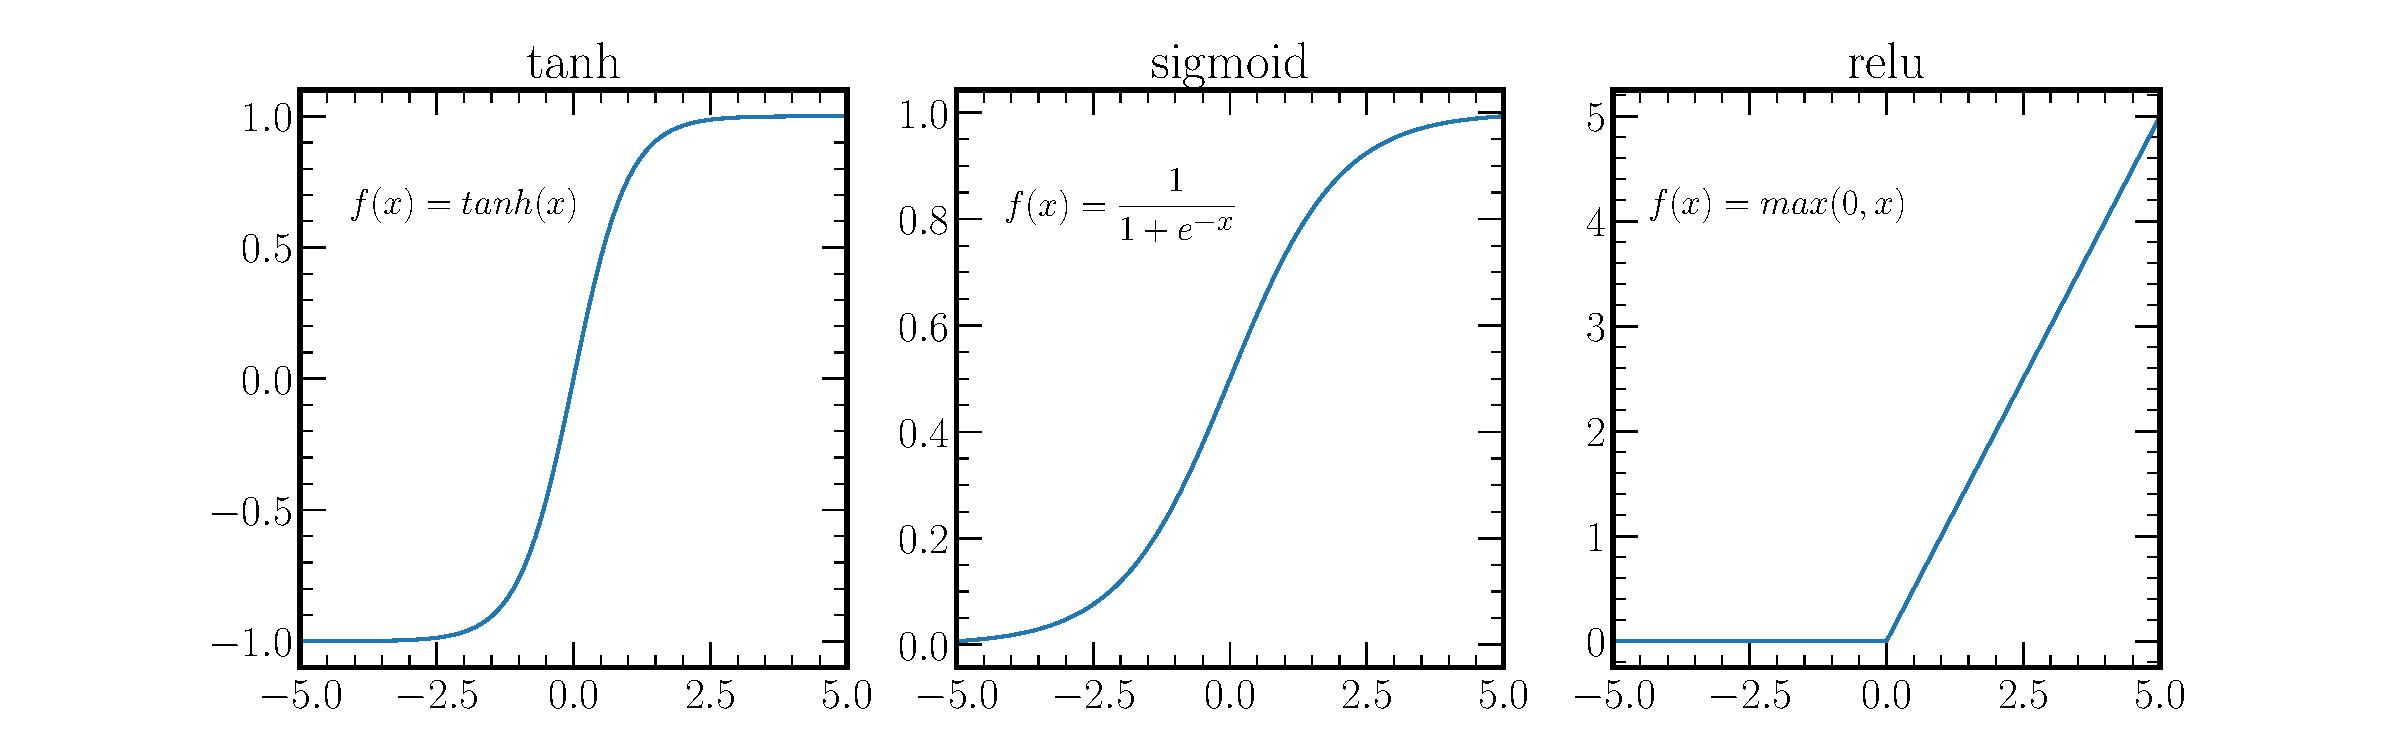
\includegraphics[width=\textwidth]{diagrams/6-cvn/activations.pdf}
    \caption[Common non-linear activation functions.]
    {Common non-linear activation functions used for the neurons within neural networks.}
    \label{fig:activations}
\end{figure}

\subsection{Training neural networks} %%%%%%%%%%%%%%%%%%%%%%%%%%%%%%%%%%%%%%%%%%%%%%%%%%%%%%%%%%%%
\label{sec:cvn_theory_training} %%%%%%%%%%%%%%%%%%%%%%%%%%%%%%%%%%%%%%%%%%%%%%%%%%%%%%%%%%%%%%%%%%

The process of supervised training of a neural network uses labelled data to iteratively find the
optimal weights and biases (network parameters) that maximise the network performance. In order to
quantify the performance, we must define a \emph{loss function} $E(\vec{w})$, where $\vec{w}$ is
the vector of network parameters, describing the difference between the network output and the
true label. For a given input data point $(\vec{x}_{i}, y_{i})$, where $\vec{x}_{i}$ are the input
parameters and $y_{i}$ is the known truth label, the network generates an output
$\hat{y}_{i}(\vec{w})$. Using this notation, we can then construct loss functions suitable for
different tasks.

In the case of a simple binary classification task, the most commonly used function is the
\emph{cross-entropy}:
\begin{equation} % BINARY CROSS-ENTROPY EQUATION %
    E(\vec{w})=
    -\displaystyle\sum_{i=1}^{n}y_{i}\log\hat{y}_{i}(\vec{w})+
    (1-y_{i})\log[1-\hat{y}_{i}(\vec{w})],
    \label{eq:binary_cross_entropy}
\end{equation}
where the number of data points is given by $n$. For a classification task where the number of
classes is greater than two $y$ can take on $M$ values. In this case we redefine each data point
so that $y$ is instead a vector $y_{im}$ such that
\begin{equation} % ONE-HOT EQUATION %
    y_{im}=
    \begin{cases}
        1 & \text{if $y_{i}=m$} \\
        0 & \text{otherwise.}   \\
    \end{cases}
\end{equation}
This is commonly named a \emph{one-hot} vector. The cross-entropy then becomes
\begin{equation} % CATEGORICAL CROSS-ENTROPY EQUATION %
    E(\vec{w})=
    -\displaystyle\sum_{i=1}^{n}\displaystyle\sum_{m=0}^{M-1}y_{im}\log\hat{y}_{im}
    (\vec{w})+(1-y_{im})\log[1-\hat{y}_{im}(\vec{w})].
    \label{eq:categorical_cross_entropy}
\end{equation}
For a regression task predicting a continuous output variable, the \emph{mean-squared error} is
most often used as the loss function:
\begin{equation} % MEAN-SQUARED ERROR LOSS EQUATION %
    E(\vec{w})=
    \frac{1}{n}\displaystyle\sum_{i=1}^{n}(y_{i}-
    \hat{y}_{i}(\vec{w}))^{2}.
    \label{eq:mse}
\end{equation}

To find the optimal network parameters for the given task we can iteratively minimise the loss
function until it converges to its minimum (or in reality a local minimum that performs well).
This is done by updating the network parameters at each iteration $t$ to move in the direction of
the gradient of the loss function using an update rule:
\begin{equation} % UPDATE EQUATION %
    \vec{w}_{t+1}=\vec{w}_{t}-\eta_{t}\nabla_{\vec{w}}E(\vec{w}),
    \label{eq:update_rule}
\end{equation}
where $\eta_{t}$ is the \emph{learning rate} which determines the size of the step that is taken
at each iteration. This methodology is known as \emph{gradient descent} and is illustrated in
Fig.~\ref{fig:gradient_descent}.

\begin{figure} % GRADIENT DESCENT DIAGRAM %
    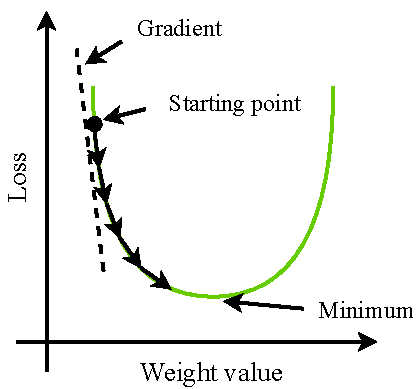
\includegraphics[width=0.5\textwidth]{diagrams/6-cvn/gradient_descent.pdf}
    \caption[Illustration of the gradient descent process.]
    {Simplified illustration of the gradient descent process. Shown is the case for a loss
        function dependent on a single weight.}
    \label{fig:gradient_descent}
\end{figure}

Therefore, in order to use gradient descent, we require that the gradient of the loss function
with respect to the parameters of the network can be calculated. Doing this for each parameter at
every iteration would render neural networks impossible to use due to the vast computational
requirements. Instead, an innovative application of the chain rule in an algorithm called
\emph{backpropagation} (backprop) is used~\cite{werbos1974}. Here we follow the derivation of the
four main equations of backpropagation from Ref.~\cite{mehta2019}.

For a network containing $L$ layers, we can index the individual layers using $l=1,\dots,L$. The
weight associated with the connection between the $k$-th neuron in layer $l-1$ and the $j$-th
neuron in layer $l$ can be denoted as $w^{l}_{jk}$. The bias of the layer $l$ neuron is written as
$b^{l}_{j}$. The activation of the $j$-th neuron in layer $l$ is then related to the outputs from
the previous layer by
\begin{equation} % PREVIOUS LAYER EQUATION %
    a^{l}_{j}=\sigma(z^{l}_{j})=\sigma\left(\sum_{k}w^{l}_{jk}a^{l-1}_{k}+b^{l}_{j}\right).
    \label{eq:feedforward}
\end{equation}

The change in the loss function with respect to the linear weighted sum $z^{l}_{j}$ of the $j$-th
neuron in the last layer $L$ can be used to define the error:
\begin{equation} % PREVIOUS LAYER EQUATION %
    \Delta^{L}_{j}=\frac{\partial E}{\partial z^{L}_{j}}.
\end{equation}
Similarly the error on any neuron $j$ in any layer $l$ is given by
\begin{equation} % BACKPROP EQUATION 1 %
    \Delta^{l}_{j}=\frac{\partial E}{\partial z^{l}_{j}}=\frac{\partial E}{\partial a^{l}_{j}}
    \sigma '(z^{l}_{j}),
    \label{eq:backprop_1}
\end{equation}
with $\sigma '$ denoting the derivative of the non-linear activation function. As $\partial
    b^{l}_{j}/\partial z^{l}_{j}=1$, the error can also be viewed as the partial derivative of the
loss function with respect to the bias:
\begin{equation} % BACKPROP EQUATION 2 %
    \Delta^{l}_{j}=\frac{\partial E}{\partial z^{l}_{j}}
    =\frac{\partial E}{\partial b^{l}_{j}}\frac{\partial b^{l}_{j}}{\partial z^{l}_{j}}
    =\frac{\partial E}{\partial b^{l}_{j}}.
    \label{eq:backprop_2}
\end{equation}

Using the chain rule and the fact that the error on neurons in layer $l$ only depends on the
activation of neurons in the following layer $l+1$, we can write
\begin{align} % BACKPROP EQUATION 3 %
    \begin{split}
        \Delta^{l}_{j} &=\frac{\partial E}{\partial z^{l}_{j}}
        =\sum_{k}\frac{\partial E}{\partial z^{l+1}_{k}}
        \frac{\partial z^{l+1}_{k}}{\partial z^{l}_{j}} \\
        &=\sum_{k}\Delta^{l+1}_{k}\frac{\partial z^{l+1}_{k}}{\partial z^{l}_{j}} \\
        &=\left(\sum_{k}\Delta^{l+1}_{k}w^{l+1}_{kj}\right)\sigma '(z^{l}_{j}).
    \end{split}
    \label{eq:backprop_3}
\end{align}
Additionally, the differential of the cost function with respect to the weight $w^{l}_{jk}$ can be
written as
\begin{equation} % BACKPROP EQUATION 4 %
    \frac{\partial E}{\partial w^{l}_{jk}}
    =\frac{\partial E}{\partial z^{l}_{j}}\frac{\partial z^{l}_{j}}{\partial w^{l}_{jk}}
    =\Delta^{l}_{j}a^{l-1}_{k}.
    \label{eq:backprop_4}
\end{equation}

The full backpropagation algorithm then proceeds as follows:
\begin{enumerate}
    \item After calculating the activations $a^{1}_{j}$ for all neurons in the input layer, use
          the feed-forward architecture of the network to calculate all activations at every layer
          using Eq.~\ref{eq:feedforward}.
    \item Use Eq.~\ref{eq:backprop_1} to calculate the error of the top layer neurons. Both the
          derivative of the loss function and the activation function is required for this step.
    \item Use Eq.~\ref{eq:backprop_2} to `backpropagate' the error through the network from the
          top layer to the input layer to find all $\Delta^{l}_{j}$ values.
    \item Calculate the gradients for all the weights and biases using Eq.~\ref{eq:backprop_3} and
          Eq.~\ref{eq:backprop_4}.
\end{enumerate}
As can be seen, a single activation finding \emph{forward pass} followed by a single error
propagating \emph{backward pass}  is all that's required to calculate the gradients for all
weights and biases within the network. This incredibly efficient procedure allows for the use of
gradient descent to train neural networks.

\subsection{Convolutional neural networks} %%%%%%%%%%%%%%%%%%%%%%%%%%%%%%%%%%%%%%%%%%%%%%%%%%%%%%%
\label{sec:cvn_theory_conv} %%%%%%%%%%%%%%%%%%%%%%%%%%%%%%%%%%%%%%%%%%%%%%%%%%%%%%%%%%%%%%%%%%%%%%

The broad category of deep learning covers multiple neural network techniques spanning a range of
application fields such as computer vision, speech recognition and natural language processing. By
stacking many layers on top of each other into a `deep' network, these methods offer increased
problem-solving capacity by allowing higher-order non-linear functions to form. Therefore, instead
of requiring hand-engineered features as input, these techniques work to extract the most powerful
features from raw data. Here we outline just the technique used in this work; the convolutional
neural network.

At their core, a CNN makes use of a mathematical operation called \emph{convolution}, which either
entirely or in part replaces the simple vector multiplication seen in fully-connected networks as
introduced in Section~\ref{sec:cvn_theory_basics}. This change makes CNNs incredibly powerful for
applications using grid-like data such as computer vision tasks.

Using standard CNN terminology, the discrete convolution between the \emph{input} $x$ and the
\emph{kernel} $w$ is given by
\begin{equation}
    f_{i}=(x*w)_{i}=\sum^{\infty}_{j=-\infty}x_{j}w_{i-j},
\end{equation}
where the output $f$ is commonly referred to as the \emph{feature map}. In typical applications,
the input is a two-dimensional array of input values $X$. Therefore, both the kernel $W$ and the
resulting feature map $F$ also become two-dimensional. In this case the convolution operation
becomes
\begin{equation}
    F_{i}=(X*W)_{i,j}=\sum_{m}\sum_{n}X_{i+m,j+n}W_{m,n},
    \label{eq:conv}
\end{equation}
where the infinite sum has been replaced with a discrete sum over two-dimensional elements.
Normally the output feature map is then passed through a non-linear activation function. Analogous
to the simple neural network weights $\vec{w}$ first described in Eq.~\ref{eq:network}, the
elements of $W_{m,n}$ can be trained to maximise the network performance (minimise the loss).

To illustrate this operation Fig.~\ref{fig:conv_input} gives examples of a $4 \times 4$ input grid
and a $3 \times 3$ kernel. The output feature map is generated by sliding the kernel across both
dimensions of the input grid, summing the products of all associated elements at each step
according to Eq.~\ref{eq:conv}, as shown in Fig.~\ref{fig:conv_operation}.

\begin{figure} % CONV INPUTS DIAGRAM %
    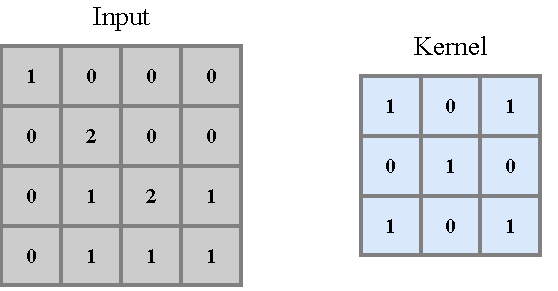
\includegraphics[width=0.6\textwidth]{diagrams/6-cvn/conv_input.pdf}
    \caption[Example of an input grid and kernel.]
    {Example of an input grid (left) and kernel (right). The specific kernel shown is sensitive to
        x-shaped features}
    \label{fig:conv_input}
\end{figure}

\begin{figure} % CONV OPERATION DIAGRAM %
    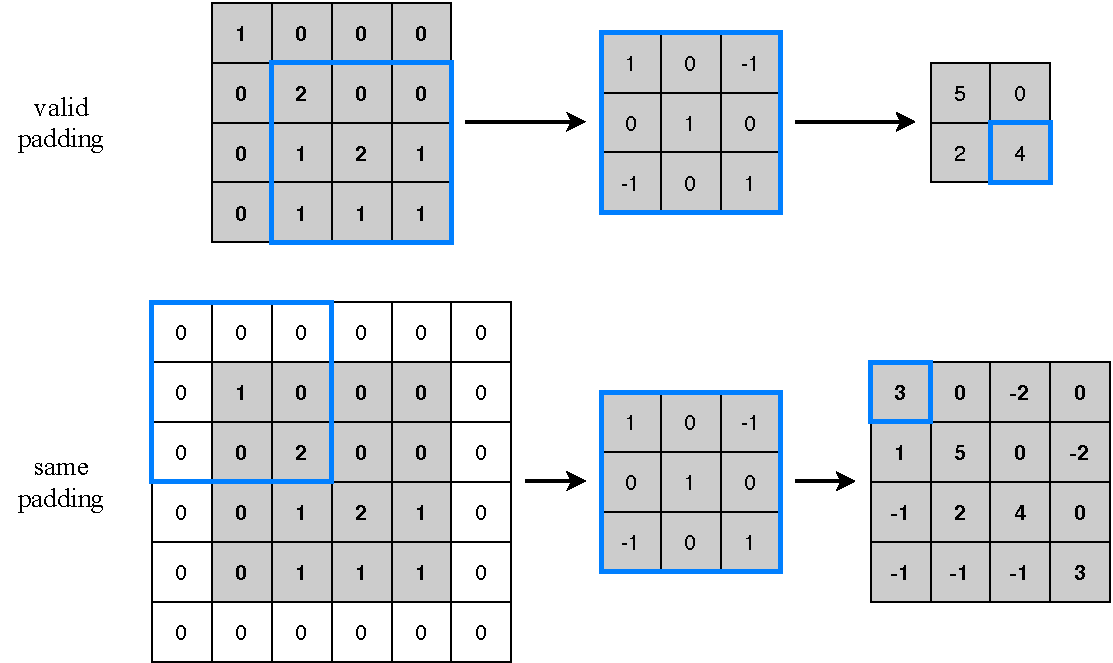
\includegraphics[width=0.8\textwidth]{diagrams/6-cvn/conv_operation.pdf}
    \caption[Example of convolutional operation.]
    {Example of a $\mathrm{stride}=1$ convolutional operation involving the input grid and kernel
        from Fig.~\ref{fig:conv_input}. Both the operation for the case of \emph{valid} (top) and
        \emph{same} (bottom) padding is shown. The blue square in the top-left of the output
        feature maps indicates the output generated from the specific operation shown.}
    \label{fig:conv_operation}
\end{figure}

Two additional parameters that affect the output size of the feature map are also introduced in
Fig.~\ref{fig:conv_operation}. The \emph{stride} and the \emph{padding}. The stride governs how
far the kernel moves at each step while the padding decides if the input grid is padded with zeros
around its border. If $L$ is the size of the input (both height and width) and $K$ is the kernel
size, the output feature map size $O$ is given by
\begin{equation}
    O=\frac{(L-K+2P)}{S}+1,
    \label{eq:conv_size}
\end{equation}
where $S$ is the stride, and $P$ is the amount of zero padding.

The other key operation used in CNNs is pooling. Pooling layers coarse-grain the spatial
information of the input via down-sampling to reduce the number of network parameters which is
typically high for CNNs. \emph{Max pooling} or \emph{average pooling} are the two common ways this
is achieved. In both cases, the input is first divided into rectangular regions, and then either
the maximum or average value of the region is used as output, for max and average pooling
respectively. This is illustrated in Fig.\ref{fig:pooling}.

\begin{figure} % POOLING DIAGRAM %
    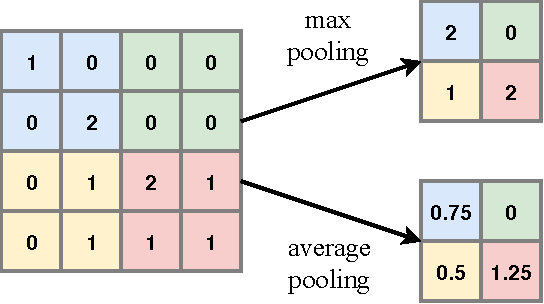
\includegraphics[width=0.6\textwidth]{diagrams/6-cvn/pooling.pdf}
    \caption[Example of pooling operation.]
    {Example of both a max and average $2 \times 2$ pooling operation with $\mathrm{stride}=2$.}
    \label{fig:pooling}
\end{figure}

Taking inspiration from how neurons behave in the visual cortex of animals~\cite{lecun2015}, small
kernels are generally used that only scan over a small spatial patch of the input at any one time.
When combined with the loss of absolute position information that pooling produces, it highlights
a key feature of CNNs. They exhibit translational invariance and respect the local structure
contained within the input. In simpler terms, they do not care wherein the input image a
particular feature exists, just that it exists.

\subsubsection*{CNN architectures}

In 2012 the AlexNet CNN lowered the error rate of the ubiquitous ImageNet classification
task~\cite{deng2009} from 28\% to 16\%~\cite{krizhevsky2012}. Since this breakthrough, the
standard CNN has adopted the same architecture. Multiple convolutional layers are stacked on top
of each other, periodically interspersed with pooling layers. Once the output feature map size no
longer allows for additional pooling, one or more fully-connected layers are added before the
final output layer, as shown in Fig.~\ref{fig:conv_diagram}.

\begin{figure} % CONV DIAGRAM %
    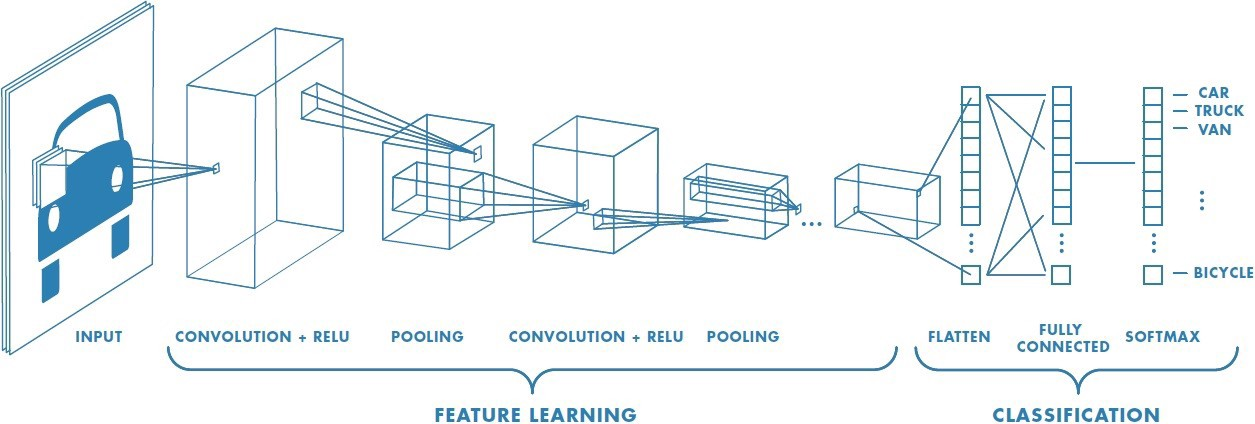
\includegraphics[width=\textwidth]{diagrams/6-cvn/conv_diagram.jpeg}
    \caption[Typical CNN architecture]
    {Illustration of a typical CNN architecture, containing convolutional, pooling and
        fully-connected layers before the final output layer.}
    \label{fig:conv_diagram}
\end{figure}

Led by research teams at the technology giants, improvements upon this standard architecture have
been made. Initially, this involved the addition of extra convolutional layers to form a deeper
network as VGG did in 2014~\cite{simonyan2014}. Separately, the \emph{inception module} introduced
by GoogLeNet~\cite{szegedy2015} the same year allowed for different scales of features to be
explored using the concept of a \emph{network within a network}.

As the size of CNNs increased, it was found that the gradients on the lower layers of the network
were found to decrease. This sometimes had the effect of the gradient \emph{vanishing} from these
layers preventing learning. To counter this problem ResNet~\cite{he2016_original, he2016_improved}
introduced residual connections, skipping specific layers and allowing for a large gradient to
reach the affected lower layers during backpropagation. Recently the inception module and ResNet
ideas have been combined~\cite{szegedy2016}, and there has been a significant push for efficient
rather than just deeper networks~\cite{sandler2018,tan2019}. The repeating layout of layers that
form the above networks, often referred to as \emph{blocks}, are shown in Fig.~\ref{fig:blocks}.

\begin{figure} % BLOCKS DIAGRAM %
    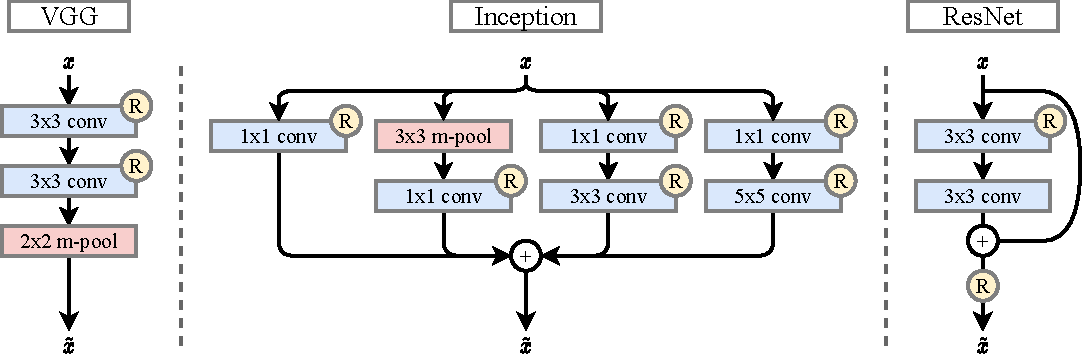
\includegraphics[width=\textwidth]{diagrams/6-cvn/blocks.pdf}
    \caption[Common CNN architecture blocks]
    {Common blocks used within CNN architectures, taking $x$ as input and producing $\tilde{x}$ as
        output through operations whose flow is outlined via the arrows. The blue and red boxes
        represent convolutional and pooling layers respectively, with the size of the operation
        shown. The circular yellow $R$ indicates the use of the ReLU activation function.}
    \label{fig:blocks}
\end{figure}

\subsection{Regularisation} %%%%%%%%%%%%%%%%%%%%%%%%%%%%%%%%%%%%%%%%%%%%%%%%%%%%%%%%%%%%%%%%%%%%%%
\label{sec:cvn_theory_reg} %%%%%%%%%%%%%%%%%%%%%%%%%%%%%%%%%%%%%%%%%%%%%%%%%%%%%%%%%%%%%%%%%%%%%%%

A key challenge for supervised machine learning techniques is ensuring the algorithm can
generalise to new, previously unseen datasets. This can be difficult when for a deep neural
network containing millions of trainable parameters, it can become easy for the network to learn
the specific features and noise of the training dataset. This process is called \emph{overfitting}
and is common when training CNNs. Methods used within this work to prevent this from happening are
outlined below, all of which are commonly referred to as \emph{regularisation} techniques.

\subsubsection*{Stochastic Gradient Descent} %%%%%%%%%%%%%%%%%%%%%%%%%%%%%%%%%%%%%%%%%%%%%%%%%%%%%

The process outlined so far of updating the network weights at each training iteration using the
gradient calculated over the full dataset is called \emph{batch training}. It is instead much more
common to calculate an approximation to the gradient at each iteration using a \emph{minibatch} of
the full dataset. This is done by considering just a subset of the training data with a size
commonly referred to as the \emph{batch size} and typically equal to a power of two for
computational reasons.

This modification to standard gradient descent is called \emph{stochastic gradient descent} as it
introduces stochasticity to the training process, and has two main advantages. Firstly the
computational speed of each iteration is significantly reduced, and crucially the memory
requirements lowered. Secondly, the additional noise introduced decreases the chance that the
minimisation will get stuck in a local minimum suited to overfitting the training dataset.

\subsubsection*{Early stopping} %%%%%%%%%%%%%%%%%%%%%%%%%%%%%%%%%%%%%%%%%%%%%%%%%%%%%%%%%%%%%%%%%%

\emph{Early stopping} is a simple procedure which prevents overfitting from affecting the final
generalised performance of the network. During training, the training dataset is commonly iterated
over multiple times, with each iteration called an \emph{epoch}. By evaluating the error on an
independent \emph{validation} dataset at the end of each epoch, the point at which overfitting
begins can be determined, as shown in Fig.~\ref{fig:early_stopping}. At this point, the training
is stopped to return the best possible generalised model. In practice, it is common only to stop
training after $n$ number of epochs have passed with no validation error improvement.

\begin{figure} % EARLY STOPPING DIAGRAM %
    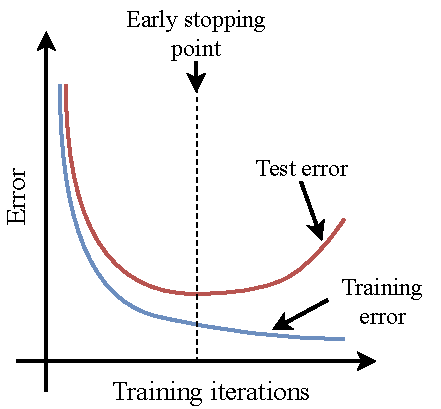
\includegraphics[width=0.5\textwidth]{diagrams/6-cvn/early_stopping.pdf}
    \caption[Illustration of the early stopping procedure.]
    {Illustration of the early stopping procedure. Initially both the training and test error
        decreases, but, at some point the test error will start to increase due to overfitting, at
        this point the training is stopped.}
    \label{fig:early_stopping}
\end{figure}

\subsubsection*{Batch normalisation} %%%%%%%%%%%%%%%%%%%%%%%%%%%%%%%%%%%%%%%%%%%%%%%%%%%%%%%%%%%%%

The training of a neural network is found to work best when the inputs of each neuron are centred
on zero with respect to the bias of the neuron. This is because large input values can cause
saturation of the activation function and subsequent \emph{vanishing} of the associated gradient,
reducing the ability of the network to learn. To counter this, \emph{batch normalisation}
introduces layers that standardise the inputs using the mean and variance calculated over each
minibatch~\cite{ioffe2015}. This not only speeds up training by preventing the \emph{vanishing} of
gradients but also reduces overfitting by again using the stochasticity of the minibatch.

\subsubsection*{Dropout} %%%%%%%%%%%%%%%%%%%%%%%%%%%%%%%%%%%%%%%%%%%%%%%%%%%%%%%%%%%%%%%%%%%%%%%%%

\emph{Dropout} is another simple technique to reduce overfitting~\cite{hinton2012}. At each
training iteration, each neuron has a probability $p$ to be \emph{dropped out} and ignored for
that iterations calculations. This is illustrated in \ref{fig:dropout}. By ignoring a subset of
the neurons at each iteration it makes it harder for the network to form the particularly strong
connections between neurons that are usually responsible for overfitting, leading to greater
generalisation.

\begin{figure} % DROPOUT DIAGRAM %
    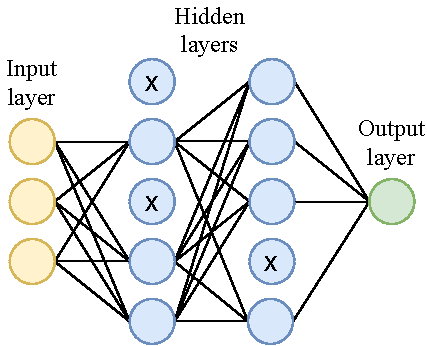
\includegraphics[width=0.6\textwidth]{diagrams/6-cvn/dropout.pdf}
    \caption[Illustration of dropout.]
    {Example of dropout applied to the network shown in Fig.~\ref{fig:network}. Neurons are
        randomly \emph{dropped out} and not considered at each training step. This reduces the
        strong correlations between neurons that can lead to overfitting.}
    \label{fig:dropout}
\end{figure}

\section{A baseline implementation for CHIPS} %%%%%%%%%%%%%%%%%%%%%%%%%%%%%%%%%%%%%%%%%%%%%%%%%%%%
\label{sec:cvn_baseline} %%%%%%%%%%%%%%%%%%%%%%%%%%%%%%%%%%%%%%%%%%%%%%%%%%%%%%%%%%%%%%%%%%%%%%%%%

MAYBE REFER TO THE BASELINE JUST AT CHIPSNET

The output from a water Cherenkov detector such as \chips is effectively a simple \emph{image} of
each event (neutrino interaction) where the number of collected photoelectrons (p.e) and hit times
are known for each PMT. Therefore, it is a natural fit for these event \emph{images} to be
analysed by a CNN which was primarily developed for computer vision tasks on images and other
grid-like input data.

For this purpose, a python based software package named \emph{chipsnet}~\cite{chipsnet2020} has
been developed. By using the high-level \emph{application programming interfaces}, (APIs) provided
by the Tensorflow framework (initially built by Google)~\cite{tf2015}, a full pipeline including
data preparation, network training, and final network performance evaluation has been implemented.

In this section, an outline for the baseline implementation built into chipsnet for applying CNNs
to \chips is presented. The following section then details the specifics surrounding the
individual cosmic rejection, beam classification and energy estimation applications.

\subsection{Baseline inputs} %%%%%%%%%%%%%%%%%%%%%%%%%%%%%%%%%%%%%%%%%%%%%%%%%%%%%%%%%%%%%%%%%%%%%
\label{sec:cvn_baseline_inputs} %%%%%%%%%%%%%%%%%%%%%%%%%%%%%%%%%%%%%%%%%%%%%%%%%%%%%%%%%%%%%%%%%%

The primary difficulty in the application of CNNs to the \chips project is determining how to map
an event captured on a cylindrical surface to a rectangular grid. Furthermore, this must be done
in such a way as not to distort the event topology which could make it harder for the CNN to
learn. To solve this problem, this work takes inspiration and then builds upon the ideas outlined
in Ref.~\cite{theodore2016}. Simply put, an event is projected onto a two-dimensional grid as
though it was \emph{viewed} from its estimated interaction vertex position. The primary motivation
behind this is to remove the detector shape from having any impact and to focus on the underlying
event topology and Cherenkov profiles. Other, competing representations that do not perform as
well are outlined in Section~\ref{sec:cvn_baseline_alt} for completeness.

To estimate the interaction vertex position for each event, the top-scoring seed from the
\emph{seeding} process introduced in Section~\ref{sec:cvn_old_reco} is used. This procedure unlike
the full likelihood fit requires no track hypothesis and typically takes a much reduced 0.5
seconds per event on a standard batch farm computing node. The seed estimated vertex position
resolutions (truth-seed) for a sample of expected beam events are shown in
Fig.~\ref{fig:explore_true_reco_vtx}. Although the $x$ component of the position tends to be
estimated closer to the downstream wall of the detector than reality, this should not increase
event distortions greatly as these are primarily driven by the $y$ and $z$ components not parallel
to the beamline.

\begin{figure} % HOUGH VTX RES DIAGRAM %
    \includegraphics[width=\textwidth]{diagrams/6-cvn/chipsnet/explore_true_reco_vtx.pdf}
    \caption[Seed interaction vertex resolutions.]
    {$Truth - seed$ interaction vertex position resolution, split by component. The large negative
        tail for the $x$ component shows the tendency of the seeding procedure to estimate the $x$
        component closer to the downstream detector wall than reality.}
    \label{fig:explore_true_reco_vtx}
\end{figure}

Using $\theta$ and $\phi$ components calculated from the estimated interaction vertex position
facing along the x-axis (downstream), all hit PMTs within an event are projected onto a $64 \times
    64$ grid. This procedure results in a mapping between all PMTs and their associated bins within
the grid, which is used to generate two event \emph{maps}. Firstly, a \emph{hit-charge} map where
each bin value is given by the sum of the total collected charge (p.e) from all PMTs mapped to
that bin. Secondly, a \emph{hit-time} map where each bin value is given by the first hit time from
all the PMTs mapped to that bin (corrected, so the first hit time in the event is at zero).

By design, the Hough transform used in the seeding procedure uses the estimated interaction vertex
position to generate the transform space. Therefore, by re-binning the transform space to a $64
    \times 64$ grid a third \emph{hough-height} map is also generated for each event. This event map
aims to provide a complementary but different representation of the event where Cherenkov rings
are instead represented as peaks, which may allow for additional powerful features to be learnt.

All three event map: hit-charge, hit-time and hough-height, are down-sampled (from 32-bit floats)
using 8-bit encoding. This not only significantly reduces the storage requirements but also
dramatically increases the speed with which data can be loaded during training. For each map type,
a range over which to encode from zero up to a \emph{cap-point} is chosen. This is selected to
minimise the number of values that are capped at the maximum encoded value of 255, which otherwise
could lead to the loss of crucial information within the data. Table.~\ref{tab:encoding} shows the
cap-points, and associated percentage of values capped for each map type, while
Fig.~\ref{fig:explore_8_bit_range} shows the distribution of values for each map across the
encoded range.

\begin{table}
    \begin{tabular}{lllll}
        Event map    & Cap-point & Capped percentage \\
        \midrule
        hit-charge   & 25 p.e    & 0.10\%            \\
        hit-time     & 120 ns    & 0.15\%            \\
        hough-height & 3500 p.e  & 0.23\%            \\
    \end{tabular}
    \caption{Table showing the cap-points (maximum value of the encoding range) and the associated
        percentage of values that are capped at the maximum 8-bit value of 255 as a consequence.}
    \label{tab:encoding}
\end{table}

\begin{figure} % 8-BIT DIAGRAM %
    \includegraphics[width=0.6\textwidth]{diagrams/6-cvn/chipsnet/explore_8_bit_range.pdf}
    \caption[explore 8 bit range short]
    {The distribution of encoded 8-bit values for the hit charge, hit time and Hough value
        channels. Note the \emph{overflow} bin at an 8-bit value of $256$.}
    \label{fig:explore_8_bit_range}
\end{figure}

Example events expected within \chips are shown in Fig.~\ref{fig:explore_nuel_ccres_event} for a
CC resonant $\nu_{e}$ event, in Fig.~\ref{fig:explore_numu_ccdis_event} for a CC DIS $\nu_{\mu}$
event, in Fig.~\ref{fig:explore_nuel_ncdis_event} for a NC DIS event, and in
Fig.~\ref{fig:explore_cosmic_event} for a cosmic muon event.

\begin{figure} % NUEL EVENT DIAGRAM %
    \includegraphics[width=\textwidth]{diagrams/6-cvn/chipsnet/explore_nuel_ccres_event.pdf}
    \caption[Example of a CC resonant $\nu_{e}$ event.]
    {Three channel representation of a CC resonant $\nu_{e}$ event. Initiated by a $\nu_{e}$ of
        energy \unit{3.3}{\GeV}, the final state particles above the Cherenkov threshold include a
        $e^{-}$ of energy \unit{2.8}{\GeV} and a \unit{0.3}{\GeV} $\pi^{0}$.}
    \label{fig:explore_nuel_ccres_event}
\end{figure}

\begin{figure} % NUMU EVENT DIAGRAM %
    \includegraphics[width=\textwidth]{diagrams/6-cvn/chipsnet/explore_numu_ccdis_event.pdf}
    \caption[Example of a CC DIS $\nu_{\mu}$ event.]
    {Three channel representation of a CC DIS $\nu_{\mu}$ event. Initiated by a $\nu_{\mu}$ of
        energy \unit{3.5}{\GeV}, the final state particles above the Cherenkov threshold include a
        $\mu^{-}$ of energy \unit{1.9}{\GeV}, a proton of \unit{2.0}{\GeV} and a \unit{0.2}{\GeV}
        $\pi^{-}$.}
    \label{fig:explore_numu_ccdis_event}
\end{figure}

\begin{figure} % NC EVENT DIAGRAM %
    \includegraphics[width=\textwidth]{diagrams/6-cvn/chipsnet/explore_nuel_ncdis_event.pdf}
    \caption[Example of a NC DIS event.]
    {Three channel representation of a NC DIS event. Initiated by a $\nu_{e}$ of energy
        \unit{9.3}{GeV}, the final state particles above the Cherenkov threshold include a proton
        of \unit{2.6}{\GeV} and a \unit{2.5}{\GeV} $\pi^{-}$.}
    \label{fig:explore_nuel_ncdis_event}
\end{figure}

\begin{figure} % COSMIC MUON EVENT DIAGRAM %
    \includegraphics[width=\textwidth]{diagrams/6-cvn/chipsnet/explore_cosmic_event.pdf}
    \caption[Example of a cosmic muon event.]
    {Three channel representation of a cosmic muon event, containing a $\mu^{-}$ of energy
        \unit{2.9}{\GeV}.}
    \label{fig:explore_cosmic_event}
\end{figure}

\subsection{Baseline architecture} %%%%%%%%%%%%%%%%%%%%%%%%%%%%%%%%%%%%%%%%%%%%%%%%%%%%%%%%%%%%%%%
\label{sec:cvn_baseline_arch} %%%%%%%%%%%%%%%%%%%%%%%%%%%%%%%%%%%%%%%%%%%%%%%%%%%%%%%%%%%%%%%%%%%%

An illustrative diagram of the baseline network architecture is shown in Fig.~\ref{fig:chipsnet}.
It is based on the VGG network (16 layer variant) previously mentioned in
Section.~\ref{sec:cvn_previous} and detailed in Ref.~\cite{simonyan2014}. There are a few key and
major differences from the network outlined in the literature, these are discussed below.

\begin{figure} % CHIPSNET DIAGRAM %
    \includegraphics[width=0.9\textwidth]{diagrams/6-cvn/chipsnet.pdf}
    \caption[chipsnet short]
    {Illustrative diagram of the baseline chipsnet network architecture. }
    \label{fig:chipsnet}
\end{figure}

\begin{itemize}
    \item Each of the three event maps: hit-charge, hit-time, and hough-height are initially fed
          into three separate branches. Each branch contains two VGG blocks each with 2
          convolutional layers (4 convolutional layers in total). The outputs from all three
          branches are merged together using a concatenation layer before being fed to the rest of
          the network. This structure allows for the most important features from each type of
          event map to be learnt independently before the higher layers of the network learn
          combined features.

    \item Batch normalisation as described in Section.~\ref{sec:cvn_theory_reg} is included before
          the activation (ReLU) function in every convolutional layer.

    \item Squeeze-and-excitation units~\cite{hu2018} which are found to improve performance are
          included in all VGG blocks after the max-pooling operation. These units introduce extra
          parameters that aim to model the interdependencies between output feature maps, allowing
          the network to effectively weight each feature map.

    \item Dropout is included at the end of each VGG block as well as after the fully-connected
          layers. Instead of dropping individual elements, the dropout within the blocks drops
          entire kernels at each training iteration with a probability $p_{d}$. The dropout after
          the fully-connected layers, is normal, in that it drops out individual fully-connected
          neurons.

    \item Five seed output parameters are concatenated with the flattened layer before the two
          fully-connected layers. These are the three components of the estimated interaction
          vertex position ($s_{x}, s_{y}, s_{z}$) and the two components of the seed estimated
          track direction ($s_{\theta}, s_{\phi}$). This aims to provide the network with context
          as to where the input event maps where generated from within the detector and any power
          that can be gained from an estimate to the track direction.
\end{itemize}

In software the network architecture is implemented using the Keras API built into
Tensorflow~\cite{chollet2015}. This allows for simple pre-defined common layers to be easily
structured into the required architecture. Other, more advanced architectures were tested which
did not produce any performance improvements, but are outlined in
Section~\ref{sec:cvn_baseline_alt} for completeness.

\subsection{Baseline outputs} %%%%%%%%%%%%%%%%%%%%%%%%%%%%%%%%%%%%%%%%%%%%%%%%%%%%%%%%%%%%%%%%%%%%
\label{sec:cvn_baseline_outputs} %%%%%%%%%%%%%%%%%%%%%%%%%%%%%%%%%%%%%%%%%%%%%%%%%%%%%%%%%%%%%%%%%

The specific outputs for the different networks are detailed in Section.~\ref{sec:cvn_specific},
however they all share a common methodology which is described here. Many CNN applications are
found to benefit from learning multiple tasks (regression and classification) from the same
inputs. This is commonly believed to be the case as the learning process of multiple tasks leads
to a more generalised representation of the inputs where the features learnt for one task can
improve the performance of another. This is called \emph{multi-task} learning and is used
extensively in this work.

In order to train the network a loss function $E_{tot}$ must be defined that combines the
individual loss functions for each task $E_{i}$. This can be done simply by using a linear
weighted sum, sum that
\begin{equation}
    E_{tot} = \sum_{i=1}^{i=N}w_{i}E_{i},
    \label{eq:multi_simple}
\end{equation}
where $N$ is the number of tasks and $w_{i}$ are the associated weights. In this work this is
referred to as the \emph{simple} multi-task output. As the final network performance can strongly
depend on the relative weighting between loss functions, optimising these simple weights can be
difficult and time consuming. Especially when the return values from the different loss functions
are many order of magnitude different. Another approach outlined in Ref.~\cite{kendall2018} is to
learn the optimal weighting between loss functions by introducing any additional trainable
parameter for each $\sigma_{i}$, such that
\begin{equation}
    E_{tot}= \sum_{i=1}^{i=N}\frac{1}{2\sigma_{i}^2}E_{i}+ \log\sigma_{i}.
\end{equation}
In this work we refer to this as the \emph{learnt} multi-task output.

As will be shown in Section.~\ref{sec:cvn_specific}, both methods are found to be advantageous in
different scenario's. The ability to quickly test either method with any number of outputs was a
key goal behind the software implementation of chipsnet. This allows for rapid iteration of
multi-task testing, which is especially important when trial-and-error seems to be the only way to
determine if something will work. CLASSIC DOWNSIDE OF THE BLACK BOX, SOMETIMES IT WORKS SOMETIMES
NOT!!!

\subsection{Baseline Training} %%%%%%%%%%%%%%%%%%%%%%%%%%%%%%%%%%%%%%%%%%%%%%%%%%%%%%%%%%%%%%%%%%%
\label{sec:cvn_baseline_training} %%%%%%%%%%%%%%%%%%%%%%%%%%%%%%%%%%%%%%%%%%%%%%%%%%%%%%%%%%%%%%%%
% Describe the training sample used, typical training times, epochs, batch sizes, hyperparamters
% The basic categorisation we are training for etc...

- When used by the CNN the values are additionally converted to a float between 0 and 1.
- Makes training across multiple graphics processing units (GPUs) easy to implement.
- We use the Tensorflow dataset API which creates an efficient input pipeline for training data,
allowing it to be loaded on the fly at training time. Impossible to load everything into memory.
- The input files are loaded and random events are loaded into memory decoded and any
manipulations applied before use in training.
- The use of parrallelism allows for all CPU cores (and threads) to be used for loading and
preprocessing data for the GPU batch training process. Preloading the data so it is ready for when
it is needed.
- To optimise data storage and training speed at the training stage all inputs are encoded using
8-bits, with the scaling determined to saturate for each channel ~0.001!!! SHOW PLOT Bottleneck at
training becomes the loading of data on the fly and not the actual network calculations done on
the GPUs.
- Input data is scaled for all channels to be between [0, 1]
- Training data is split into a train and validation dataset 95-5\% split.
- We apply augmentation to the images apply a random factor scaling to each input pixel of
2\% for all channels. Clipping any negative values this produces back to zero.
- Mini-batch training strategy was used.
- The SHERPA hyperparameter tuning framework was used for hyperparameter tuning.
- We use a learning rate determined from hyperparamter studies to converge well,reducing the
learning rate at each step according to
\begin{equation}
    l_{e}=\frac{l_{0}}{1+c_{d}n_{e}}
\end{equation}
where $c_{d}$ is the coefficient of decay set to be 0.5 and $n_{e}$ is the epoch number
- Implement early stopping
- learning rate = 0.0001
- learning rate decay = 0.5
- precision policy = mixed float 16
- Augment 2\% on all channels

- GIVE TABLE OF FULL LIST OF HYPERPARAMETERS THAT ARE TUNABLE USING SHERPA

\subsection{Baseline evaluation} %%%%%%%%%%%%%%%%%%%%%%%%%%%%%%%%%%%%%%%%%%%%%%%%%%%%%%%%%%%%%%%%%
\label{sec:cvn_baseline_eval} %%%%%%%%%%%%%%%%%%%%%%%%%%%%%%%%%%%%%%%%%%%%%%%%%%%%%%%%%%%%%%%%%%%%
% Introduce testing sample, event weighting and metrics used for determining the best model
% How we combine nuel and numu results into a combined score

- Explain the primary task we are trying to solve
- List secondary objective as well
- Which metrics will we use to judge success for each of these objectives
- How the test events are scaled (weighted) with oscillations and expected beam and cosmic nums.
- Completely independent of the training dataset
- Present a simple exploration of the testing dataset key components and distributions.
- Expected number of events table etc...
- Primary goal is to classify the neutrino flavour nuel CC, numu CC or NC
- Secondary goal is to then classify the individual interaction mode (QEL, RES, DIS etc...) these
will have different energy resolutions and systematic uncertainties, so seperation can provide
increased sensitivity.

I can then explain how we will evaluate the network using a separate testing dataset weighted and
stuff etc and which metrics are used to determine the performance of both the primary and
secondary objectives.

- See signal interactions peaked closely near score values of unity and the backgrounds lie close
to the zero score as expected.

\begin{figure} % OSC FLUXES DIAGRAM %
    \includegraphics[width=0.8\textwidth]{diagrams/6-cvn/chipsnet/explore_osc_fluxes.pdf}
    \caption[Weighted spectrum of testing sample events.]
    {The weighted spectrum of events contained within the testing sample. The weighting is
        designed to mimic the expected beam neutrino event spectrum of the \chips detector by
        combining the expected unoscillated flux with cross-sections and standard oscillation
        probabilities. Shown in blue, green and olive are the survived CC $\nu_{\mu}$, appeared CC
        $\nu_{e}$ and the intrinsic beam CC $\nu_{e}$ spectra respectively, binned in terms of
        their neutrino energy. Shown in red is the NC event spectra binned in terms of the energy
        of the hadronic system (excluding the outgoing neutrino energy) to better represent the
        energy visible to the detector.}
    \label{fig:explore_osc_fluxes}
\end{figure}

\begin{figure} % STACK INT TYPES DIAGRAM %
    \includegraphics[width=0.8\textwidth]{diagrams/6-cvn/chipsnet/explore_stacked_int_types.pdf}
    \caption[Weighted spectrum of interaction types within the testing sample.]
    {The weighted spectrum of events contained within the testing sample separated by interaction type.}
    \label{fig:explore_stacked_int_types}
\end{figure}

\begin{figure} % SIMPLE CUTS DIAGRAM %
    \includegraphics[width=0.8\textwidth]{diagrams/6-cvn/chipsnet/explore_simple_cuts.pdf}
    \caption[explore simple cuts short]
    {explore simple cuts long}
    \label{fig:explore_simple_cuts}
\end{figure}

\subsection{Baseline Alternatives} %%%%%%%%%%%%%%%%%%%%%%%%%%%%%%%%%%%%%%%%%%%%%%%%%%%%%%%%%%%%%%%
\label{sec:cvn_baseline_alt} %%%%%%%%%%%%%%%%%%%%%%%%%%%%%%%%%%%%%%%%%%%%%%%%%%%%%%%%%%%%%%%%%%%%%
% Introduce testing sample, event weighting and metrics used for determining the best model

As a nice sidenote I can then just mention a few things such as the input sample type, different
architectures and different input representations that where tested to get to this final baseline
implementation. Noting this interesting things and trying to explain why they may be physically.

- truncated versions of the other networks so they have approximately the same number of parameters
to train for making a good comparison.

\begin{figure} % ARCH DIAGRAM %
    \includegraphics[width=\textwidth]{diagrams/6-cvn/arch.pdf}
    \caption[arch short]
    {arch long}
    \label{fig:arch}
\end{figure}

vgg: 17,225,296 (88ms)
inception: 16,893,216 (192ms)
resnet: 16,526,288 (112ms)
inception-resnet: 17,145,238 (209ms)

\begin{figure} % ARCHITECTURE NUEL EFF CURVES DIAGRAM %
    \includegraphics[width=0.6\textwidth]{diagrams/6-cvn/chipsnet/arch_nuel_eff_curves.pdf}
    \caption[arch nuel eff curves short]
    {vgg=solid, inception=dashed, resnet=dotted, inception-resnet=dot-dash}
    \label{fig:arch_nuel_eff_curves}
\end{figure}

\begin{figure} % ARCHITECTURE NUEL COMP CURVES DIAGRAM %
    \includegraphics[width=0.8\textwidth]{diagrams/6-cvn/chipsnet/arch_nuel_comp_curves.pdf}
    \caption[arch nuel comp curves short]
    {vgg=solid, inception=dashed, resnet=dotted, inception-resnet=dot-dash}
    \label{fig:arch_nuel_comp_curves}
\end{figure}

- Nuel-> ROC-AUC: 0.82559, PRC-AUC: 0.71155, S-Eff: 0.87661, S-Pur: 0.36928
- FOM1-> 0.46510, 0.93000, 53.44422, 8.34671, 15.75487, 0.67485, 0.68920
- FOM2-> 13.44645, 0.98500, 31.21664, 1.57028, 3.81933, 0.39418, 0.85277

- Nuel-> ROC-AUC: 0.82519, PRC-AUC: 0.70632, S-Eff: 0.86992, S-Pur: 0.37332
- FOM1-> 0.45910, 0.91500, 53.20954, 9.73154, 14.92970, 0.67188, 0.68331
- FOM2-> 13.47965, 0.98500, 28.04995, 1.43802, 2.89217, 0.35419, 0.86627

- Nuel-> ROC-AUC: 0.82444, PRC-AUC: 0.68789, S-Eff: 0.86926, S-Pur: 0.37417
- FOM1-> 0.44511, 0.91000, 54.46409, 11.50537, 18.18029, 0.68772, 0.64723
- FOM2-> 12.22026, 0.98000, 32.56108, 2.77151, 4.32813, 0.41115, 0.82099

- Nuel-> ROC-AUC: 0.82444, PRC-AUC: 0.69946, S-Eff: 0.87369, S-Pur: 0.34882
- FOM1-> 0.44448, 0.90500, 52.61119, 10.90981, 15.11323, 0.66433, 0.66906
- FOM2-> 13.48962, 0.98500, 23.98040, 0.96809, 2.19211, 0.30280, 0.88356

\begin{figure} % FLUX TRAINING SAMPLE DIAGRAM %
    \includegraphics[width=0.6\textwidth]{diagrams/6-cvn/chipsnet/explore_flux_sample.pdf}
    \caption[explore flux sample short]
    {explore flux sample long}
    \label{fig:explore_flux_sample}
\end{figure}

\begin{figure} % UNIFORM TRAINING SAMPLE DIAGRAM %
    \includegraphics[width=0.6\textwidth]{diagrams/6-cvn/chipsnet/explore_uniform_sample.pdf}
    \caption[explore uniform sample short]
    {explore uniform sample long}
    \label{fig:explore_uniform_sample}
\end{figure}

\begin{figure} % BOTH TRAINING SAMPLE DIAGRAM %
    \includegraphics[width=0.6\textwidth]{diagrams/6-cvn/chipsnet/explore_both_sample.pdf}
    \caption[explore both sample short]
    {explore both sample long}
    \label{fig:explore_both_sample}
\end{figure}

\begin{figure} % SAMPLE FLUX OUTPUT DIAGRAM %
    \includegraphics[width=0.6\textwidth]{diagrams/6-cvn/chipsnet/sample_flux_output_values.pdf}
    \caption[sample flux output values short]
    {sample flux output values long}
    \label{fig:sample_flux_output_values}
\end{figure}

\begin{figure} % SAMPLE UNIFORM OUTPUT DIAGRAM %
    \includegraphics[width=0.6\textwidth]{diagrams/6-cvn/chipsnet/sample_uniform_output_values.pdf}
    \caption[sample uniform output values short]
    {sample uniform output values long}
    \label{fig:sample_uniform_output_values}
\end{figure}

\begin{figure} % SAMPLE BOTH OUTPUT DIAGRAM %
    \includegraphics[width=0.6\textwidth]{diagrams/6-cvn/chipsnet/sample_both_output_values.pdf}
    \caption[sample both output values short]
    {sample both output values long}
    \label{fig:sample_both_output_values}
\end{figure}

\begin{figure} % SAMPLE NUEL EFF CURVES DIAGRAM %
    \includegraphics[width=0.6\textwidth]{diagrams/6-cvn/chipsnet/sample_nuel_eff_curves.pdf}
    \caption[sample nuel eff curves short]
    {both=solid, flux=dashed, uniform=dotted}
    \label{fig:sample_nuel_eff_curves}
\end{figure}

\begin{figure} % SAMPLE NUEL COMP CURVES DIAGRAM %
    \includegraphics[width=0.8\textwidth]{diagrams/6-cvn/chipsnet/sample_nuel_comp_curves.pdf}
    \caption[sample nuel comp curves short]
    {both=solid, flux=dashed, uniform=dotted}
    \label{fig:sample_nuel_comp_curves}
\end{figure}

- Nuel-> ROC-AUC: 0.82559, PRC-AUC: 0.71155, S-Eff: 0.87661, S-Pur: 0.36928
- FOM1-> 0.46510, 0.93000, 53.44422, 8.34671, 15.75487, 0.67485, 0.68920
- FOM2-> 13.44645, 0.98500, 31.21664, 1.57028, 3.81933, 0.39418, 0.85277

- Nuel-> ROC-AUC: 0.81488, PRC-AUC: 0.56769, S-Eff: 0.79933, S-Pur: 0.34677
- FOM1-> 0.33905, 0.82500, 49.50120, 26.12079, 15.63656, 0.62506, 0.54243
- FOM2-> 8.44226, 0.92500, 36.01710, 11.59853, 6.60268, 0.45479, 0.66430

- Nuel-> ROC-AUC: 0.82063, PRC-AUC: 0.63426, S-Eff: 0.83421, S-Pur: 0.36814
- FOM1-> 0.38628, 0.84000, 52.60971, 19.59654, 18.26900, 0.66431, 0.58148
- FOM2-> 10.10769, 0.96000, 30.52599, 4.49055, 4.63030, 0.38545, 0.76995

- New ideas with x+ x- mapping in Ref.~\cite{berns2020}
- Fraction of deposited charge in endcaps = 0.4769380479133997

\begin{equation} % ONE-HOT EQUATION %
    X_{\pm}=
    \begin{cases}
        1-\chi_{\mp} & (z \geq 0) \\
        \chi_{\pm}   & (z < 0)
    \end{cases}
\end{equation}

\begin{equation} % ONE-HOT EQUATION %
    \chi_{\pm}=W(\rho,z)\frac{\pi\pm\phi}{2\pi}
\end{equation}

\begin{equation}
    W(\rho,z)=\sqrt{\frac{\rho^{2}-2R\abs{z}+RH}{R^{2}+RH}}
\end{equation}

where R and Z are the radius and height of the detector cylinder and W is chosen for constant
surface density.

- Turns out removing the distortions of not viewing the event from the vertex is the most important
thing!!!

- Approaches in the past for event classification using CNNs for water cherenkov detectors have
taken a few Approaches to generating the input image representation.
- Projecting onto a 2d surface "outside" the detector

- Nuel-> ROC-AUC: 0.82509, PRC-AUC: 0.70686, S-Eff: 0.87786, S-Pur: 0.35433
- FOM1-> 0.46118, 0.93000, 52.98765, 8.61419, 15.27335, 0.66908, 0.68927
- FOM2-> 13.26595, 0.98500, 29.74203, 1.43964, 3.58684, 0.37556, 0.85543

- Nuel-> ROC-AUC: 0.82178, PRC-AUC: 0.67486, S-Eff: 0.87439, S-Pur: 0.29114
- FOM1-> 0.42202, 0.95500, 50.65626, 10.27209, 15.82963, 0.63948, 0.65995
- FOM2-> 12.53864, 0.99000, 29.40728, 1.75353, 3.74706, 0.37123, 0.84243

- Nuel-> ROC-AUC: 0.82116, PRC-AUC: 0.66987, S-Eff: 0.86660, S-Pur: 0.29764
- FOM1-> 0.41895, 0.94500, 50.97483, 10.86474, 16.45768, 0.64350, 0.65104
- FOM2-> 12.22739, 0.99000, 28.43808, 1.74364, 3.66555, 0.35900, 0.84019

\begin{figure} % REPR NUEL EFF CURVES DIAGRAM %
    \includegraphics[width=0.6\textwidth]{diagrams/6-cvn/chipsnet/repr_nuel_eff_curves.pdf}
    \caption[repr nuel eff curves short]
    {v=solid, o=dashed, i=dotted}
    \label{fig:repr_nuel_eff_curves}
\end{figure}

\begin{figure} % REPR NUEL COMP CURVES DIAGRAM %
    \includegraphics[width=0.8\textwidth]{diagrams/6-cvn/chipsnet/repr_nuel_comp_curves.pdf}
    \caption[repr nuel comp curves short]
    {v=solid, o=dashed, i=dotted}
    \label{fig:repr_nuel_comp_curves}
\end{figure}

\begin{figure} % CHANNEL NUEL EFF CURVES DIAGRAM %
    \includegraphics[width=0.6\textwidth]{diagrams/6-cvn/chipsnet/channel_nuel_eff_curves.pdf}
    \caption[channel nuel eff curves short]
    {c=solid, ct=dashed, cth=dotted, cth-stacked=dot-dash}
    \label{fig:channel_nuel_eff_curves}
\end{figure}

\begin{figure} % CHANNEL NUEL COMP CURVES DIAGRAM %
    \includegraphics[width=0.8\textwidth]{diagrams/6-cvn/chipsnet/channel_nuel_comp_curves.pdf}
    \caption[channel nuel comp curves short]
    {c=solid, ct=dashed, cth=dotted, cth-stacked=dot-dash}
    \label{fig:channel_nuel_comp_curves}
\end{figure}

- Nuel-> ROC-AUC: 0.82377, PRC-AUC: 0.68935, S-Eff: 0.86860, S-Pur: 0.35681
- FOM1-> 0.43601, 0.91000, 53.71070, 12.22704, 17.60798, 0.67821, 0.64289
- FOM2-> 12.70378, 0.99000, 20.73912, 0.76294, 1.90217, 0.26187, 0.88613

- Nuel-> ROC-AUC: 0.82509, PRC-AUC: 0.70686, S-Eff: 0.87786, S-Pur: 0.35433
- FOM1-> 0.46118, 0.93000, 52.98765, 8.61419, 15.27335, 0.66908, 0.68927
- FOM2-> 13.26595, 0.98500, 29.74203, 1.43964, 3.58684, 0.37556, 0.85543

- Nuel-> ROC-AUC: 0.82559, PRC-AUC: 0.71155, S-Eff: 0.87661, S-Pur: 0.36928
- FOM1-> 0.46510, 0.93000, 53.44422, 8.34671, 15.75487, 0.67485, 0.68920
- FOM2-> 13.44645, 0.98500, 31.21664, 1.57028, 3.81933, 0.39418, 0.85277

- Nuel-> ROC-AUC: 0.82521, PRC-AUC: 0.70198, S-Eff: 0.87180, S-Pur: 0.38254
- FOM1-> 0.45819, 0.91500, 55.18628, 11.56662, 17.17741, 0.69684, 0.65753
- FOM2-> 12.66558, 0.99000, 24.37959, 1.35104, 2.35408, 0.30784, 0.86807

\section{Specific implementations} %%%%%%%%%%%%%%%%%%%%%%%%%%%%%%%%%%%%%%%%%%%%%%%%%%%%%%%%%%%%%%%
\label{sec:cvn_specific} %%%%%%%%%%%%%%%%%%%%%%%%%%%%%%%%%%%%%%%%%%%%%%%%%%%%%%%%%%%%%%%%%%%%%%%%%

\subsection{Cosmic muon rejection} %%%%%%%%%%%%%%%%%%%%%%%%%%%%%%%%%%%%%%%%%%%%%%%%%%%%%%%%%%%%%%%
\label{sec:cvn_specific_cosmic} %%%%%%%%%%%%%%%%%%%%%%%%%%%%%%%%%%%%%%%%%%%%%%%%%%%%%%%%%%%%%%%%%%

\subsubsection*{Escaping particles} %%%%%%%%%%%%%%%%%%%%%%%%%%%%%%%%%%%%%%%%%%%%%%%%%%%%%%%%%%%%%%

\subsection{Beam classification}%%%%%%%%%%%%%%%%%%%%%%%%%%%%%%%%%%%%%%%%%%%%%%%%%%%%%%%%%%%%%%%%%%
\label{sec:cvn_specific_beam} %%%%%%%%%%%%%%%%%%%%%%%%%%%%%%%%%%%%%%%%%%%%%%%%%%%%%%%%%%%%%%%%%%%%

\subsubsection*{Categorisation} %%%%%%%%%%%%%%%%%%%%%%%%%%%%%%%%%%%%%%%%%%%%%%%%%%%%%%%%%%%%%%%%%%

\begin{figure} % T_ALL_CAT SAMPLE DIAGRAM %
    \includegraphics[width=0.6\textwidth]{diagrams/6-cvn/chipsnet/explore_t_all_cat.pdf}
    \caption[explore t all cat short]
    {explore t all cat long}
    \label{fig:explore_t_all_cat}
\end{figure}

\begin{figure} % T_NC_COMB_CAT SAMPLE DIAGRAM %
    \includegraphics[width=0.6\textwidth]{diagrams/6-cvn/chipsnet/explore_t_nc_comb_cat.pdf}
    \caption[explore t nc comb cat short]
    {explore t nc comb cat long}
    \label{fig:explore_t_nc_comb_cat}
\end{figure}

\begin{figure} % T_COMB_CAT SAMPLE DIAGRAM %
    \includegraphics[width=0.6\textwidth]{diagrams/6-cvn/chipsnet/explore_t_comb_cat.pdf}
    \caption[explore t comb cat short]
    {explore t comb cat long}
    \label{fig:explore_t_comb_cat}
\end{figure}

\begin{figure} % CAT NUEL EFF CURVES DIAGRAM %
    \includegraphics[width=0.6\textwidth]{diagrams/6-cvn/chipsnet/cat_nuel_eff_curves.pdf}
    \caption[cat nuel eff curves short]
    {cat nuel eff curves long}
    \label{fig:cat_nuel_eff_curves}
\end{figure}

\begin{figure} % CAT NUEL COMP CURVES DIAGRAM %
    \includegraphics[width=0.8\textwidth]{diagrams/6-cvn/chipsnet/cat_nuel_comp_curves.pdf}
    \caption[cat nuel comp curves short]
    {cat nuel comp curves long}
    \label{fig:cat_nuel_comp_curves}
\end{figure}

\begin{figure} % CAT NUMU EFF CURVES DIAGRAM %
    \includegraphics[width=0.6\textwidth]{diagrams/6-cvn/chipsnet/cat_numu_eff_curves.pdf}
    \caption[cat numu eff curves short]
    {cat numu eff curves long}
    \label{fig:cat_numu_eff_curves}
\end{figure}

\begin{figure} % CAT NUMU COMP CURVES DIAGRAM %
    \includegraphics[width=0.8\textwidth]{diagrams/6-cvn/chipsnet/cat_numu_comp_curves.pdf}
    \caption[cat numu comp curves short]
    {cat numu comp curves long}
    \label{fig:cat_numu_comp_curves}
\end{figure}

\subsubsection*{Counting primary particles} %%%%%%%%%%%%%%%%%%%%%%%%%%%%%%%%%%%%%%%%%%%%%%%%%%%%%%

- DUNE tried counting exclusive final state particles (protons, chargedpions, neutral pions)
- As the different final states will have different energy resolutions and sytematic
uncertainties, it may be possible for a future analysis to improve the oscillation paramter
sensitivity by indentifying subsamples with specific topologies.
- Primary partile scores can be combined to give compounded scores for the exclusive final state
selections.

\begin{figure} % BEAM NUEL EFF CURVES DIAGRAM %
    \includegraphics[width=0.6\textwidth]{diagrams/6-cvn/chipsnet/beam_nuel_eff_curves.pdf}
    \caption[beam nuel eff curves short]
    {beam nuel eff curves long}
    \label{fig:beam_nuel_eff_curves}
\end{figure}

\begin{figure} % BEAM NUEL COMP CURVES DIAGRAM %
    \includegraphics[width=0.8\textwidth]{diagrams/6-cvn/chipsnet/beam_nuel_comp_curves.pdf}
    \caption[beam nuel comp curves short]
    {beam nuel comp curves long}
    \label{fig:beam_nuel_comp_curves}
\end{figure}

\begin{figure} % BEAM NUMU EFF CURVES DIAGRAM %
    \includegraphics[width=0.6\textwidth]{diagrams/6-cvn/chipsnet/beam_numu_eff_curves.pdf}
    \caption[beam numu eff curves short]
    {beam numu eff curves long}
    \label{fig:beam_numu_eff_curves}
\end{figure}

\begin{figure} % BEAM NUMU COMP CURVES DIAGRAM %
    \includegraphics[width=0.8\textwidth]{diagrams/6-cvn/chipsnet/beam_numu_comp_curves.pdf}
    \caption[beam numu comp curves short]
    {beam numu comp curves long}
    \label{fig:beam_numu_comp_curves}
\end{figure}

\subsection{Energy estimation} %%%%%%%%%%%%%%%%%%%%%%%%%%%%%%%%%%%%%%%%%%%%%%%%%%%%%%%%%%%%%%%%%%%
\label{sec:cvn_specific_energy} %%%%%%%%%%%%%%%%%%%%%%%%%%%%%%%%%%%%%%%%%%%%%%%%%%%%%%%%%%%%%%%%%%

\subsubsection*{Including other energies} %%%%%%%%%%%%%%%%%%%%%%%%%%%%%%%%%%%%%%%%%%%%%%%%%%%%%%%% 

\begin{figure} % ENERGY CHAN DISTS DIAGRAM %
    \includegraphics[width=\textwidth]{diagrams/6-cvn/chipsnet/energy_chan_frac_dist.pdf}
    \caption[energy chan frac dist short]
    {energy chan frac dist long}
    \label{fig:energy_chan_frac_dist}
\end{figure}

\begin{figure} % ENERGY CHAN FRAC VS E DIAGRAM %
    \includegraphics[width=\textwidth]{diagrams/6-cvn/chipsnet/energy_chan_frac_vs_e.pdf}
    \caption[energy chan frac vs e short]
    {energy chan frac vs e long}
    \label{fig:energy_chan_frac_vs_e}
\end{figure}

\subsubsection*{Other event parameters} %%%%%%%%%%%%%%%%%%%%%%%%%%%%%%%%%%%%%%%%%%%%%%%%%%%%%%%%%% 

\begin{figure} % ENERGY PAR DISTS DIAGRAM %
    \includegraphics[width=\textwidth]{diagrams/6-cvn/chipsnet/energy_par_frac_dist.pdf}
    \caption[energy par frac dist short]
    {energy par frac dist long}
    \label{fig:energy_par_frac_dist}
\end{figure}

\begin{figure} % ENERGY PAR FRAC VS E DIAGRAM %
    \includegraphics[width=\textwidth]{diagrams/6-cvn/chipsnet/energy_par_frac_vs_e.pdf}
    \caption[energy par frac vs e short]
    {energy par frac vs e long}
    \label{fig:energy_par_frac_vs_e}
\end{figure}

\subsubsection*{Combined or split} %%%%%%%%%%%%%%%%%%%%%%%%%%%%%%%%%%%%%%%%%%%%%%%%%%%%%%%%%%%%%%% 

\begin{figure} % ENERGY SPLIT NUEL DIAGRAM %
    \includegraphics[width=\textwidth]{diagrams/6-cvn/chipsnet/final_energy_split_nuel_frac_vs_e.pdf}
    \caption[final energy split nuel frac vs e short]
    {final energy split nuel frac vs e long}
    \label{fig:final_energy_split_nuel_frac_vs_e}
\end{figure}

\begin{figure} % ENERGY SPLIT NUMU DIAGRAM %
    \includegraphics[width=\textwidth]{diagrams/6-cvn/chipsnet/final_energy_split_numu_frac_vs_e.pdf}
    \caption[final energy split numu frac vs e short]
    {final energy split numu frac vs e long}
    \label{fig:final_energy_split_numu_frac_vs_e}
\end{figure}

\section{Final combined performance} %%%%%%%%%%%%%%%%%%%%%%%%%%%%%%%%%%%%%%%%%%%%%%%%%%%%%%%%%%%%%
\label{sec:cvn_final} %%%%%%%%%%%%%%%%%%%%%%%%%%%%%%%%%%%%%%%%%%%%%%%%%%%%%%%%%%%%%%%%%%%%%%%%%%%%

\subsection{Comparison with standard methods} %%%%%%%%%%%%%%%%%%%%%%%%%%%%%%%%%%%%%%%%%%%%%%%%%%%%
\label{sec:cvn_final_comparison} %%%%%%%%%%%%%%%%%%%%%%%%%%%%%%%%%%%%%%%%%%%%%%%%%%%%%%%%%%%%%%%%%

\begin{figure} % COSMIC HISTORY DIAGRAM %
    \includegraphics[width=0.6\textwidth]{diagrams/6-cvn/chipsnet/final_cosmic_history.pdf}
    \caption[final cosmic history short]
    {final cosmic history long}
    \label{fig:final_cosmic_history}
\end{figure}

\begin{figure} % BEAM HISTORY DIAGRAM %
    \includegraphics[width=0.6\textwidth]{diagrams/6-cvn/chipsnet/final_beam_history.pdf}
    \caption[final beam history short]
    {final beam history long}
    \label{fig:final_beam_history}
\end{figure}

\begin{figure} % ENERGY HISTORY DIAGRAM %
    \includegraphics[width=0.6\textwidth]{diagrams/6-cvn/chipsnet/final_energy_history.pdf}
    \caption[final energy history short]
    {final energy history long}
    \label{fig:final_energy_history}
\end{figure}

\begin{figure} % COSMIC OUTPUTS DIAGRAM %
    \includegraphics[width=0.6\textwidth]{diagrams/6-cvn/chipsnet/final_cosmic_outputs.pdf}
    \caption[final cosmic outputs short]
    {final cosmic outputs long}
    \label{fig:final_cosmic_outputs}
\end{figure}

\begin{figure} % COSMIC OUTPUTS ZOOMED DIAGRAM %
    \includegraphics[width=0.6\textwidth]{diagrams/6-cvn/chipsnet/final_cosmic_zoomed_outputs.pdf}
    \caption[final cosmic zoomed outputs short]
    {final cosmic zoomed outputs long}
    \label{fig:final_cosmic_zoomed_outputs}
\end{figure}

\begin{figure} % ESCAPES OUTPUTS DIAGRAM %
    \includegraphics[width=0.6\textwidth]{diagrams/6-cvn/chipsnet/final_escapes_outputs.pdf}
    \caption[final escapes outputs short]
    {final escapes outputs long}
    \label{fig:final_escapes_outputs}
\end{figure}

\begin{figure} % BEAM OUTPUTS NUEL DIAGRAM %
    \includegraphics[width=0.6\textwidth]{diagrams/6-cvn/chipsnet/final_beam_nuel_outputs.pdf}
    \caption[final beam nuel outputs short]
    {final beam nuel outputs long}
    \label{fig:final_beam_nuel_outputs}
\end{figure}

\begin{figure} % BEAM OUTPUTS NUMU DIAGRAM %
    \includegraphics[width=0.6\textwidth]{diagrams/6-cvn/chipsnet/final_beam_numu_outputs.pdf}
    \caption[final beam numu outputs short]
    {final beam numu outputs long}
    \label{fig:final_beam_numu_outputs}
\end{figure}

\begin{figure} % FINAL NUEL EFF CURVES DIAGRAM %
    \includegraphics[width=0.6\textwidth]{diagrams/6-cvn/chipsnet/final_nuel_eff_curves.pdf}
    \caption[final nuel eff curves short]
    {final nuel eff curves long}
    \label{fig:final_nuel_eff_curves}
\end{figure}

\begin{figure} % FINAL NUMU EFF CURVES DIAGRAM %
    \includegraphics[width=0.6\textwidth]{diagrams/6-cvn/chipsnet/final_numu_eff_curves.pdf}
    \caption[final numu eff curves short]
    {final numu eff curves long}
    \label{fig:final_numu_eff_curves}
\end{figure}

\begin{figure} % FINAL NUEL HISTS DIAGRAM %
    \includegraphics[width=0.6\textwidth]{diagrams/6-cvn/chipsnet/final_nuel_hists.pdf}
    \caption[final nuel hists short]
    {final nuel hists long}
    \label{fig:final_nuel_hists}
\end{figure}

\begin{figure} % FINAL NUMU HISTS DIAGRAM %
    \includegraphics[width=0.6\textwidth]{diagrams/6-cvn/chipsnet/final_numu_hists.pdf}
    \caption[final numu hists short]
    {final numu hists long}
    \label{fig:final_numu_hists}
\end{figure}

\begin{figure} % FINAL COMB CAT CONFUSION DIAGRAM %
    \includegraphics[width=0.6\textwidth]{diagrams/6-cvn/chipsnet/final_comb_cat_confusion.pdf}
    \caption[final comb cat confusion short]
    {final comb cat confusion long}
    \label{fig:final_comb_cat_confusion}
\end{figure}

\begin{figure} % FINAL CC CAT CONFUSION DIAGRAM %
    \includegraphics[width=0.6\textwidth]{diagrams/6-cvn/chipsnet/final_cc_cat_confusion.pdf}
    \caption[final cc cat confusion short]
    {final cc cat confusion long}
    \label{fig:final_cc_cat_confusion}
\end{figure}

\begin{figure} % FINAL NC CAT CONFUSION DIAGRAM %
    \includegraphics[width=0.6\textwidth]{diagrams/6-cvn/chipsnet/final_nc_cat_confusion.pdf}
    \caption[final nc cat confusion short]
    {final nc cat confusion long}
    \label{fig:final_nc_cat_confusion}
\end{figure}

\begin{figure} % FINAL NUEL ENERGY DIST DIAGRAM %
    \includegraphics[width=0.6\textwidth]{diagrams/6-cvn/chipsnet/final_nuel_passed_energy_dist.pdf}
    \caption[final nuel passed energy dist short]
    {final nuel passed energy dist long}
    \label{fig:final_nuel_passed_energy_dist}
\end{figure}

\begin{figure} % FINAL NUMU ENERGY DIST DIAGRAM %
    \includegraphics[width=0.6\textwidth]{diagrams/6-cvn/chipsnet/final_numu_passed_energy_dist.pdf}
    \caption[final numu passed energy dist short]
    {final numu passed energy dist long}
    \label{fig:final_numu_passed_energy_dist}
\end{figure}

\begin{figure} % FINAL 2D ENERGY DIAGRAM %
    \includegraphics[width=0.7\textwidth]{diagrams/6-cvn/chipsnet/final_energy_2d.pdf}
    \caption[final energy 2d short]
    {final energy 2d long}
    \label{fig:final_energy_2d}
\end{figure}

\begin{figure} % FINAL NUEL ENERGY DIAGRAM %
    \includegraphics[width=0.8\textwidth]{diagrams/6-cvn/chipsnet/final_energy_nuel.pdf}
    \caption[final energy nuel short]
    {final energy nuel long}
    \label{fig:final_energy_nuel}
\end{figure}

\begin{figure} % FINAL NUMU ENERGY DIAGRAM %
    \includegraphics[width=0.8\textwidth]{diagrams/6-cvn/chipsnet/final_energy_numu.pdf}
    \caption[final energy numu short]
    {final energy numu long}
    \label{fig:final_energy_numu}
\end{figure}

DIAGRAM: Neutrino energy and estimated neutrino energy distributions on same plots.
INFO: Table of the final number of expected events and efficiency and purity of the signal at the
chosen cut value (nuel and numu)
INFO: Super-k/Dune/Nova comparison numbers for effeciencies and energy resolutions etc...
DIAGRAM: Table of how succesive cuts affect the selection of different event types

- BIG UP the difference in time it takes, as this can have a huge impact on reprocessing your full
dataset
- This allows a massive increase in the iteration rate of analysis, which can lead to an improved
rate of improvement, with less time wasted.

INFO: Need to understand the error on the number of cosmic passing the cut, is it reasonable
without a huge amount of testing data?
INFO: What are the errors on all my number values? with the stats I have?
- Having a veto in the upstream towards the beam direction would be best
- Talk about how beam muons upstream of the detector are just like cosmics and say how they could
be rejected aswell
INFO: proof that there is no topological difference between QEL and MEC if we are combining them
for the energy stuff
- Position of PMTs does not seem to be that important

- Nova gets about ~7percent energy resolution for signal events
in Ref.~\cite{jiang2019}
- Fitqun gets ~20cm vertex position resolution for nuel CCQE events
- Fitqun gets ~16cm vertex position resolution for numu CCQE events
- Fitqun gets 5.39percent to 2.58percent lepton energy resolution for nuel CCQE events
- Fitqun gets ~2.5percent lepton energy resolution for numu CCQE events
- Note all the stuff in super-k happens at lower energies ~<1.4GeV

\section{Explainability} %%%%%%%%%%%%%%%%%%%%%%%%%%%%%%%%%%%%%%%%%%%%%%%%%%%%%%%%%%%%%%%%%%%%%%%%%
\label{sec:cvn_explain} %%%%%%%%%%%%%%%%%%%%%%%%%%%%%%%%%%%%%%%%%%%%%%%%%%%%%%%%%%%%%%%%%%%%%%%%%%

\begin{figure} % COSMIC t-SNE DIAGRAM %
    \includegraphics[width=0.8\textwidth]{diagrams/6-cvn/chipsnet/final_cosmic_tsne.pdf}
    \caption[final cosmic tsne short]
    {final cosmic tsne long}
    \label{fig:final_cosmic_tsne}
\end{figure}

\begin{figure} % BEAM t-SNE DIAGRAM %
    \includegraphics[width=0.8\textwidth]{diagrams/6-cvn/chipsnet/final_beam_tsne.pdf}
    \caption[final beam tsne short]
    {final beam tsne long}
    \label{fig:final_beam_tsne}
\end{figure}

\begin{figure} % BEAM t-SNE EVENTS DIAGRAM %
    \includegraphics[width=\textwidth]{diagrams/6-cvn/chipsnet/final_beam_tsne_events.pdf}
    \caption[final beam tsne events short]
    {final beam tsne events long}
    \label{fig:final_beam_tsne_events}
\end{figure}

\begin{figure} % FRAC ENERGY EFF DIAGRAM %
    \includegraphics[width=0.6\textwidth]{diagrams/6-cvn/chipsnet/final_frac_energy_eff.pdf}
    \caption[final frac energy eff short]
    {final frac energy eff long}
    \label{fig:final_frac_energy_eff}
\end{figure}

\begin{figure} % EXPLAIN EXAMPLE EVENT DIAGRAM %
    \includegraphics[width=\textwidth]{diagrams/6-cvn/chipsnet/explain_example_event.pdf}
    \caption[explain example event short]
    {explain example event long}
    \label{fig:explain_example_event}
\end{figure}

\begin{figure} % BEAGLEBONE AND DANOUT DIAGRAM %
    \centering
    \subcaptionbox{explain cosmic activations\label{fig:explain_cosmic_activations}}{%
        \includegraphics[height=16cm]{diagrams/6-cvn/chipsnet/explain_cosmic_activations.pdf}%
    }
    \quad
    \subcaptionbox{explain beam activations\label{fig:explain_beam_activations}}{%
        \includegraphics[height=16cm]{diagrams/6-cvn/chipsnet/explain_beam_activations.pdf}%
    }
    \quad
    \subcaptionbox{explain energy activations\label{fig:explain_energy_activations}}{%
        \includegraphics[height=16cm]{diagrams/6-cvn/chipsnet/explain_energy_activations.pdf}%
    }
    \caption[The caption]
    {The caption}
\end{figure}

Initial CNN visualisation paper in Ref.~\cite{zeiler2013}
Original t-SNE paper in Ref.~\cite{maaten2008}
Grad-CAM paper in Ref.~\cite{selvaraju2017}

- For all the t-SNE stuff
- There have been plently of attempts at visualising high-dimensional data on a 2/3 dimensional
map, including Sammon mapping, Isomap, Locally Linear Embedding, Stochastic Neighbour Embedding.
- Older implementations tended to cluster all data points towards the centre of the map and proved
difficult to optimise.
- You basically set a summed probability between all points in the low-dimensional space to a
summed probability between all points in the high-dimensional space.
- t-SNE uses the student-t distribution (with a heavy tail) in the low-dimensional space to
calculate the probability. This alleviates both the crowding problem and is easier to optimise.
- Optimisation uses a simple momentum term, plus two new ideas. "Early compression" which forces
map points to stay close to each other at the start of optimisation, it is then easier for
clusters to move through each other and explore all possible global organisations of the data,
this is implemented as an L2-penalty term proportional to the sum of squared distances from the
origin, this is then removed at an iteration given as input. Secondly, "Early exaggeration" which
creates tight widely seperated clusters.
    \chapter{Implications for CHIPS}
\label{chap:implications}

\begin{comment}
CALIBRATION SENSITIVITY
TROUBLESOME EVENTS
PMT DISTRIBUTION
TIMING RESOLUTION
WATER QUALITY
POSSIBLE IMPROVEMENTS

- You have all of these possible parameters that can affect the performance (event categorisation
and kinematic reconstruction) of your WC detector

- Positioning of the detector (L, angle off-axis, overburden) *
- Size of the detector (height and radius) *
- Water quality (attenuation length, scattering vs absorption) *
- Which PMT’s you use (time resolution, charge collection) *
- How the PMT’s are positioned (percentage coverage, zones)
- Calibration quality (position, time, charge)
- Reconstruction methodology (likelihood vs CNN)
- Given these restrictions

- Only certain mine pits usable (fixes L and angle off-axis, use all overburden available)
- 12.5m radius for practical construction (fixes radius, but not height)
- Want to be able to carry the planes easily (Adds limits to PMT coverage percentage)
- Will just be looking at beam events, should not need much in the back
- PMT’s available. Due to cost etc… we fix the PMT’s we use, can still explore this space with
varying the time/charge. Can look at
\end{comment}

- but was mainly chosen to speed up iteration of network optimisation.
- This works out at 2.5m is theta and 2m in phi approx (when viewed from the centre of the detector)
    \chapter{Summary and conclusion} %%%%%%%%%%%%%%%%%%%%%%%%%%%%%%%%%%%%%%%%%%%%%%%%%%%%%%%%%%%%%%%%%
\label{chap:conclusion} %%%%%%%%%%%%%%%%%%%%%%%%%%%%%%%%%%%%%%%%%%%%%%%%%%%%%%%%%%%%%%%%%%%%%%%%%%

- It is now abundantly clear that convolutional neural networks will play a key role in the event
reconstruction and classification for \chips. What is also clear is that other water Cherenkov
neutrino experiments, which up to now have not fully embraced modern machine learning techniques
as much as other sectors of the neutrino field should do so. For a range of benefits from
increased processing time, leverage the wider computer vision ML field to make the advancements
for you while you focus on the physics analysis.

% PERFORMANCE
\begin{enumerate}
    \item Sufficient cosmic rejection for negligible beam sample contamination is achieved.
    \item Beam classification selection is surprisingly comparable to other costly experiments.
    \item Energy estimation is comparable and more generalisable compared to standard methods.
    \item Cherenkov ring and Hough peak features are clearly being learnt by the trained networks.
    \item There is clear learnt separation between categories as seen via unsupervised methods.
    \item Future work should train beam classification network on only contained events.
    \item The smearing of hit times is found to have a negligible impact on performance.
    \item Robust to charge calibration.
    \item Random PMT noise is found to have a negligible impact on performance.
    \item The input representation of the event is important for performance.
    \item The training sample must match the expected composition of events closely.
    \item The network architecture does not matter much in the context of this work.
    \item Future work should explore larger input image sizes and network architectures.
    \item Future work should study the input distribution of events in greater detail.
    \item Future work should look at using a graph convolutional network or transformers.
\end{enumerate}

\begin{figure} % CHIPS RAMP DIAGRAM %
    \includegraphics[width=\textwidth]{diagrams/4-chips/sunrise.pdf}
    \caption*{The \chipsfive detector frame at sunrise.}
\end{figure}

- Turns out neutrino water Cherenkov detectors produce as output an image-like event suitable for
modern Computer Vision techniques using Convolutional Neural Networks, a type of deep learning.

- Allowing for vastly increased speed with which analysis can be conducted and less reliance on
heavily human influenced bespoke software frameworks.

- This is fundamentally the primary event analysis task for water Cherenkov neutrino detectors.
Neutrino interactions within the detector create rings of light that are recorded on the walls of
the detector, these are used to infer the properties on the underlying neutrino interaction.
\end{mainmatter}

\begin{backmatter}
    %\bibliographystyle{resources/h-physrev}
\bibliographystyle{unsrt}
\bibliography{bibliography}
\listoffigures
\listoftables
\end{backmatter}

\end{document} % End the document 